
No website da OCDS encontra-se disponível para descarregar uma folha de cálculo em Excel com 73 red flags \cite{spreadsheet1} \cite{spreadsheet}. Cada uma destas flags é descrita através de um conjunto de diferentes parâmetros, tal como se encontra exemplificado na Tabela \ref{table:flags}.

\begin{table}[H]
	\centering
	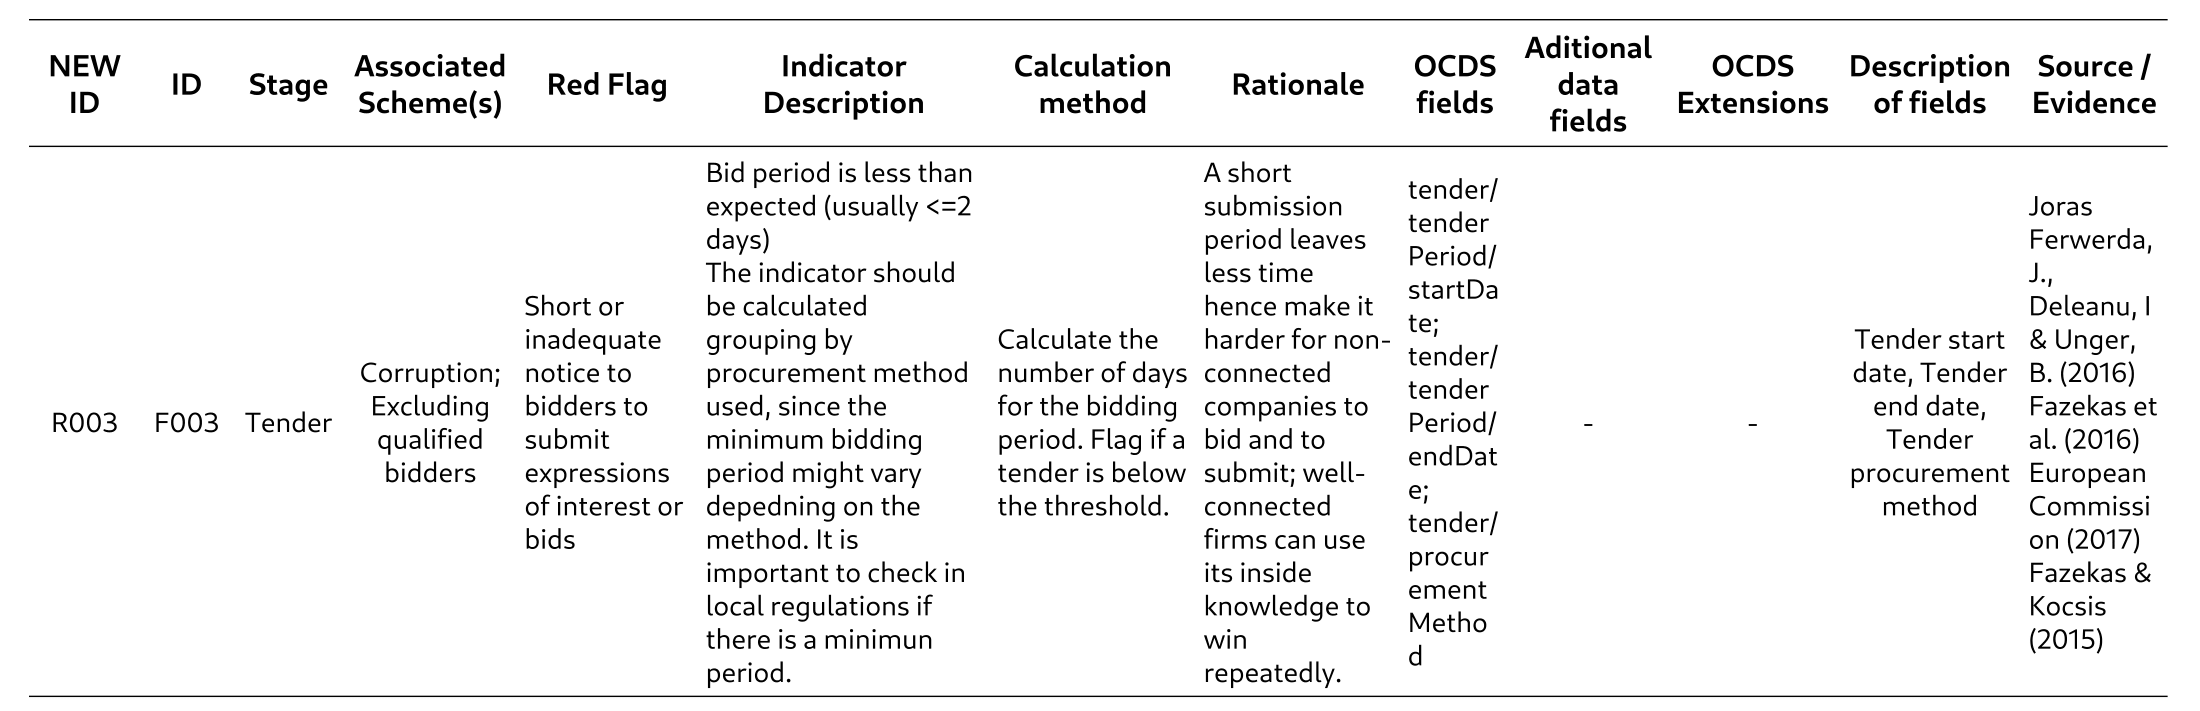
\includegraphics[width=\textwidth]{imagens/tabela_flags.png}
	\caption{Exemplo de descrição de uma flag.}
	\label{table:flags}
\end{table}







%Numa primeira instância, com o objetivo de filtrar e selecionar as flags com maior valor, foi feita uma avaliação para cada indicador, de caráter subjetivo, que incidiu sobre dois aspetos: \textbf{nível de importância} e \textbf{facilidade de implementação}. A facilidade de implementação de cada indicador foi classificado com um de três valores: \textbf{1} (difícil), \textbf{2} (médio) e \textbf{3} (fácil). Este parâmetro foi avaliado tendo em conta as variáveis disponíveis na base de dados para a construção dos indicadores e a descrição de cada indicador pois, naturalmente, existem alguns indicadores mais diretos de aplicar. O nível de importância de cada indicador foi também  classificado com um de três valores: \textbf{1} (pouco importante), \textbf{2} (importante) e \textbf{3} (muito importante). Este critério, dos dois considerados, é o que tem um cariz mais subjetivo. Finda a classificação de cada indicador, foi calculada uma média ponderada de ambas as classificações, atribuindo um peso de $0.6$ à facilidade de implementação e de $0.4$ ao nível de importância. Do conjunto total de flags, selecionaram-se todas cujo valor da média ponderada excedia o valor de 2, obtendo, assim, um subconjunto de 20 flags. De entre este subconjunto, foram desenvolvidas 6 flags.

Numa primeira instância, com o objetivo de filtrar e selecionar as flags com maior relevância, foi feita uma avaliação para cada indicador, de caráter subjetivo, que incidiu sobre dois aspectos: \textbf{nível de importância} e \textbf{facilidade de implementação}. À facilidade de implementação de cada indicador foi atribuído um de três valores: \textbf{1} (difícil), \textbf{2} (médio) e \textbf{3} (fácil). Este parâmetro foi ponderado tendo em conta as variáveis disponíveis na base de dados para a construção dos indicadores e a descrição de cada indicador, dado existirem  indicadores mais diretos de aplicar. Quanto ao nível de importância de cada indicador, foi atribuída uma classificação com um de três valores: \textbf{1} (pouco importante), \textbf{2} (importante) e \textbf{3} (muito importante). Dos dois critérios considerados, o nível de importância revela maior pendor de subjetividade. Finda a classificação de cada indicador, foi calculada uma média ponderada de ambas as classificações, tendo-se atribuído um peso de $0.6$ à facilidade de implementação e de $0.4$ ao nível de importância. Do conjunto total de flags, selecionaram-se aquelas cujo valor da média ponderada excedia o valor de 2, obtendo, assim, um subconjunto de 20 flags. De entre este subconjunto, foi possível desenvolver, no decorrer deste estágio, 6 flags.



%Além destas flags, foram desenvolvidas 3 adicionais que resultaram de discussão e troca de ideias, pois acreditava-se que agragavam valor para o resultado final. Estes indicadores foram construídos tendo em conta o CCP, as variáveis presentes na base de dados e flags definidas pela OCDS. 

A somar às flags anteriormente referidas, desenvolveram-se 3 adicionais que resultaram de discussão e troca de ideias, por se entender que tal agregaria valor ao resultado final. Estes indicadores foram construídos tendo em conta o definido no CCP, as variáveis presentes na base de dados e as flags definidas pela OCDS.

%Nas secções que se seguem, todos os indicadores establecidos pela OCDS são identificados pela letra \textbf{R} e um número, enquanto que os que foram desenvolvidos são identificados por \textbf{RF} e um número.

Nas secções que se seguem, todos os indicadores estabelecidos pela OCDS obedecem a um código alfanumérico, sendo identificados pela letra \textbf{R} e um número, enquanto os que foram desenvolvidos são identificados por \textbf{RF} e um número.

Os contratos coletados encontram-se todos guardados numa tabela denominada \textit{contratos\_basegov} que integra uma base de dados em PostgreSQL. De modo a construir os indicadores que se encontram nos capítulos seguintes, criaram-se quatro tabelas adicionais auxiliares:

\begin{my_itemize}


	\item \textbf{concursos\_publicos}: Foram inseridos nesta tabela todos os concursos públicos e as principais variáveis - \textit{id}, \textit{data\_publicacao}, \textit{contractTypes}, \textit{fundamentacao}, \textit{entidade\_adjudicante}, \textit{entidades\_contratadas}, \textit{entidades\_concorrentes}, \textit{executionPlace}, \textit{cpv} e \textit{preco\_contratual} - cuja explicação se encontra na Secção \ref{ch:variables}. A esta tabela foram adicionadas seis colunas:  \textit{nr\_entidadesconcorrentes}, \textit{tipo\_contrato}, \textit{adjudicante}, \textit{nif1}, \textit{adjudicataria} e \textit{nif2}, considerando-se que: 
	
	\begin{my_itemize}
		
		 \item \textit{nr\_entidadesconcorrentes}: o número de entidades que concorreram a um determinado concurso público.
		 
		 \item \textit{tipo\_contrato}: classifica cada um dos contratos em duas tipologias: \textbf{Bens e Serviços} ou \textbf{Obras}. 
		 
		 \item \textit{adjudicante} e \textit{nif1}: nome e número de identificação fiscal (NIF) da entidade contratante.
		 
		 \item \textit{adjudicataria} e \textit{nif2}: nome e número de identificação fiscal (NIF) da entidade contratada.
		 
	\end{my_itemize}
	
	
	\item \textbf{ajustes\_diretos}: Tabela onde foram inseridos todos os ajustes diretos em regime geral e as principais variáveis, tal como na tabela anterior. À semelhança da tabela \textit{concursos\_publicos}, também foram criadas colunas auxiliares. Não foi incluída a coluna relativa ao número de entidades concorrentes visto que esta tipologia de contrato é resultado de um convite direto, e não de um concurso aberto a qualquer entidade. Por outro lado, foi criada uma coluna \textit{criterio} que permite classificar cada contrato de acordo com o critério: critério do \textbf{valor} ou critério \textbf{material}.

	
	\item \textbf{cpv\_stat}: Esta tabela foi criada para desenvolver a flag R019. Nesta tabela registam-se os indicadores estatísticos - mínimo, $Q_1$ , $Q_2$, $Q_3$, média, desvio padrão, intervalo interquartil e máximo - relativos ao número de entidades concorrentes em concursos públicos para cada uma das \hyperref[sec:cepeves]{45 divisões\footnote{Relembra-se que a divisão do CPV consiste na caracterização de um contrato a partir dos primeiros dois dígitos deste número.} de CPV}. Na Tabela \ref{tab:cpvstat} encontra-se um exemplo de uma das linhas desta tabela. Além dos indicadores estatísticos anteriormente referidos, podem observar-se as seguintes colunas adicionais: \textbf{nec} é a soma de todas as entidades concorrentes para todos os concursos públicos celebrados pertencentes à divisão 30 do CPV; \textbf{count} é o número total de concursos públicos celebrados pertencentes à divisão 30 do CPV; \textbf{mc\_const} é a constante de Medcouple para a distribuição do número de entidades concorrentes; \textbf{lower\_fence} e \textbf{upper\_fence} dizem respeito às extremidades do boxplot para esta divisão de CPV e são calculadas utilizando as Equações \ref{eq:medatual1} e \ref{eq:medatual}. Assim, um concurso público que se destine à aquisição de máquinas e equipamentos de escritório e informática e ao qual se candidatem menos de 2 entidades ou mais de 23, é sinalizado.
	
	
	\item \textbf{preco\_stat}: a construção desta tabela obedece a uma metodologia similar à desenvolvida na das  anteriores. Contudo, em lugar de se fazer uma análise ao número de entidades concorrentes por divisão de CPV, optou-se por  uma análise do preço contratual por \hyperref[sec:cepeves]{grupo\footnote{Relembra-se que o grupo do CPV consiste na caracterização de um contrato a partir dos primeiros três dígitos deste número.} de CPV}, a fim de ter uma maior granularidade. 
	
	
\end{my_itemize}




\begin{table}[H]
	\centering
	\renewcommand{\arraystretch}{1.1}
	\resizebox{\textwidth}{!}{%
		\begin{tabular}{cccccccccccccc}
			\hline
			\textbf{cpv} & \textbf{nec} & \textbf{count} & \textbf{mean} & \textbf{std} & \textbf{min} & \textbf{q1} & \textbf{q2} & \textbf{q3} & \textbf{max} & \textbf{iqr} & \textbf{mc\_const} & \textbf{lower\_fence} & \textbf{upper\_fence} \\ \hline
			30           & 35540        & 5176           & 6.9           & 4.9          & 1            & 3           & 6           & 10          & 26           & 7            & 0.2                & 2.4                   & 22.8                  \\ \hline
		\end{tabular}%
	}
	\caption{Exemplo de uma linha da tabela \textit{cpv\_stat} para concursos públicos referentes a aquisição de máquinas e equipamentos de escritório e informática, exceto móveis e pacotes de software.}
	\label{tab:cpvstat}	
\end{table}




Na Figura \ref{fig:basededados} encontra-se um esquema da relação entre as diferentes tabelas. Para efeitos de concisão do diagrama apenas são apresentadas algumas das principais colunas. As colunas que se encontram a vermelho dizem respeito às colunas adicionais para a construção dos indicadores. É possível aceder a todos os parâmetros de um contrato que se encontre na tabela \textbf{ajustes\_diretos} ou \textbf{concursos\_publicos} através da pesquisa do identificador na tabela original \textbf{contratos\_basegov}.

\begin{figure}[H]
	\centering
	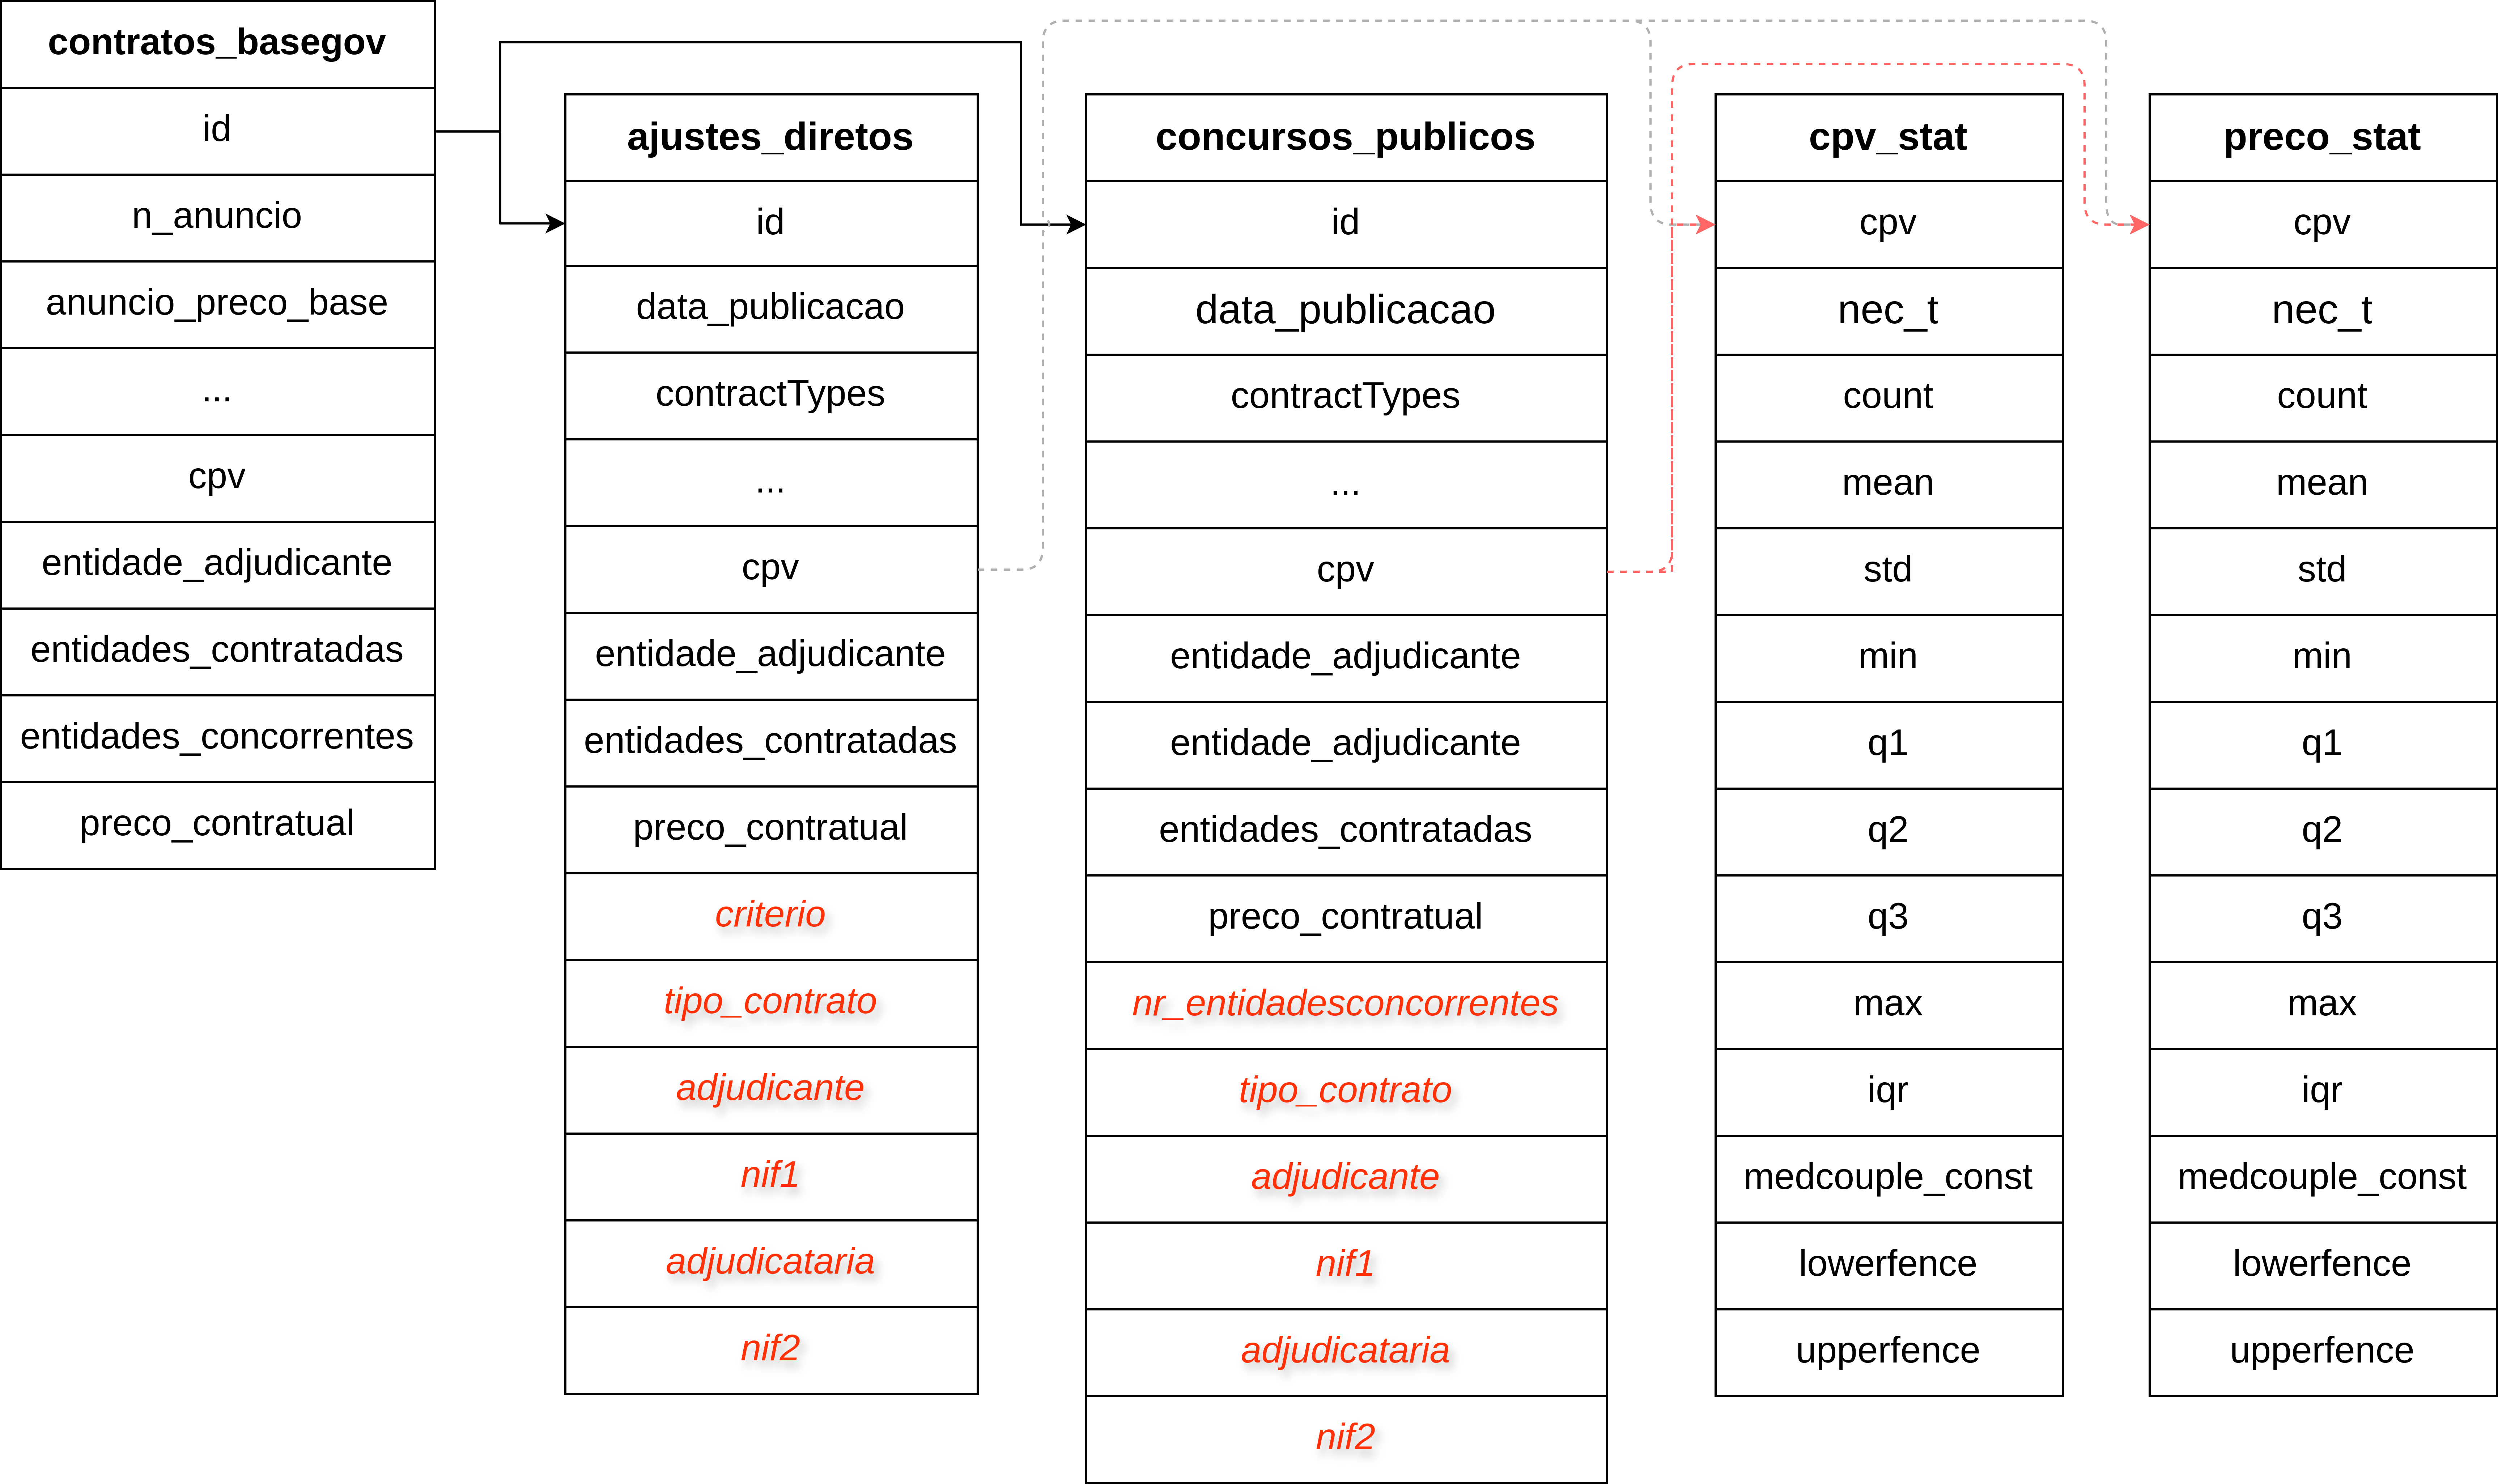
\includegraphics[width=0.9\textwidth]{imagens/basedadostabelas.png}
	\caption{Organização das tabelas da base de dados.}
	\label{fig:basededados}
\end{figure}

Nas secções sucedentes, para cada uma das flags desenvolvidas, é colocado em nota de rodapé a definição original presente na folha de Excel contruída pela OCDS.



\section{RF1: Verificação dos preços contratuais para ajustes diretos}


Este é um dos indicadores que foi desenvolvido e tem como base o CCP. Como foi apresentado anteriormente na Tabela \ref{tab:4}, os ajustes diretos, consoante o tipo de contrato\footnote{Relembra-se que o tipo de contrato foi classificado em duas categorias: \textbf{Bens e Serviços} e \textbf{Obras}.}, tem diferentes limites máximos permitidos por lei relativamente ao valor de adjudicação. A fim de poder identificar os contratos que não estão em conformidade com o CCP, procedeu-se da seguinte forma:

\begin{itemize}
	
	\item Construiu-se, a partir da tabela original, uma nova tabela \textbf{ajustes\_diretos}, onde se inseriram todos os ajustes diretos em regime geral e criou-se uma coluna, denominada \textbf{criterio}. 

	\item Para cada um dos contratos, foi identificado o artigo utilizado para fundamentar a adoção deste tipo de procedimento, presente na coluna da \textit{fundamentacao}. Se o artigo do CCP utilizado for qualquer um entre o 17º e o 22º, é atribuído ao contrato o critério do \textbf{valor} na coluna criada. Caso contrário, é atribuído o critério \textbf{material}.
	
\end{itemize}

%Primeiramente, criou-se uma nova tabela \textbf{ajustes\_diretos}, a partir da tabela original, para onde foram inseridos todos os ajustes diretos em regime geral e criou-se uma nova coluna, chamada \textbf{criterio}. De seguida, para cada um dos contratos, foi identificado o artigo utilizado para fundamentar a adoção deste tipo de procedimento, presente na coluna da fundamentação. Se o artigo utilizado for qualquer um entre o 17º e o 22º, é atribuído ao contrato o critério do \textbf{valor} na nova coluna criada. Caso contrário, é atribuído o critério \textbf{material}. 

 \begin{table}[H]
 	\centering
 	\begin{tabular}{|c|c|c|c|}
 		\hline
 		\textbf{Critério}                  & \textbf{Artigo do CCP}           & \textbf{Tipo de Contrato}           & \textbf{Valor} \\ \hline
 		\multirow{3}{*}{Critério do Valor} & \multirow{3}{*}{17º a 22º} & Aquisição de bens móveis e serviços & 20.000,00 €         \\ \cline{3-4} 
 		&                            & Empreitadas de obras públicas       & 30.000,00 €        \\ \cline{3-4} 
 		&                            & Outro tipo de contratos             & 50.000,00 € €        \\ \hline
 		Critério Material                  & 24º a 27º                  & Qualquer                            & Indefinido     \\ \hline
 	\end{tabular}
 	\caption{Valores máximos permitidos para Ajustes Diretos consoante o critério, artigo e tipo de contrato.}
 \end{table}

Posteriormente, foi necessário classificar os contratos relativamente à tipologia. Tal como se encontra representado na Tabela \ref{table:3}, os contratos podem ser classificados em duas grandes categorias: \textbf{Bens e Serviços} ou \textbf{Obras}. Contudo, na coluna referente ao tipo de contrato não é feita esta discriminação. Assim, foi adicionada uma nova coluna a esta tabela, \textbf{tipo\_contrato}, que contemplará apenas uma das duas categorias anteriormente presentes para cada contrato. Para classificar cada contrato numa destas duas categorias fez-se uma busca da palavra \textit{obra} na string presente na coluna da tipologia de contrato. Se esta palavra estivesse contida na string, o contrato era classificado como \textbf{Obras}. Caso contrário, \textbf{Bens e Serviços}. 

\begin{figure}[H]
	\centering
	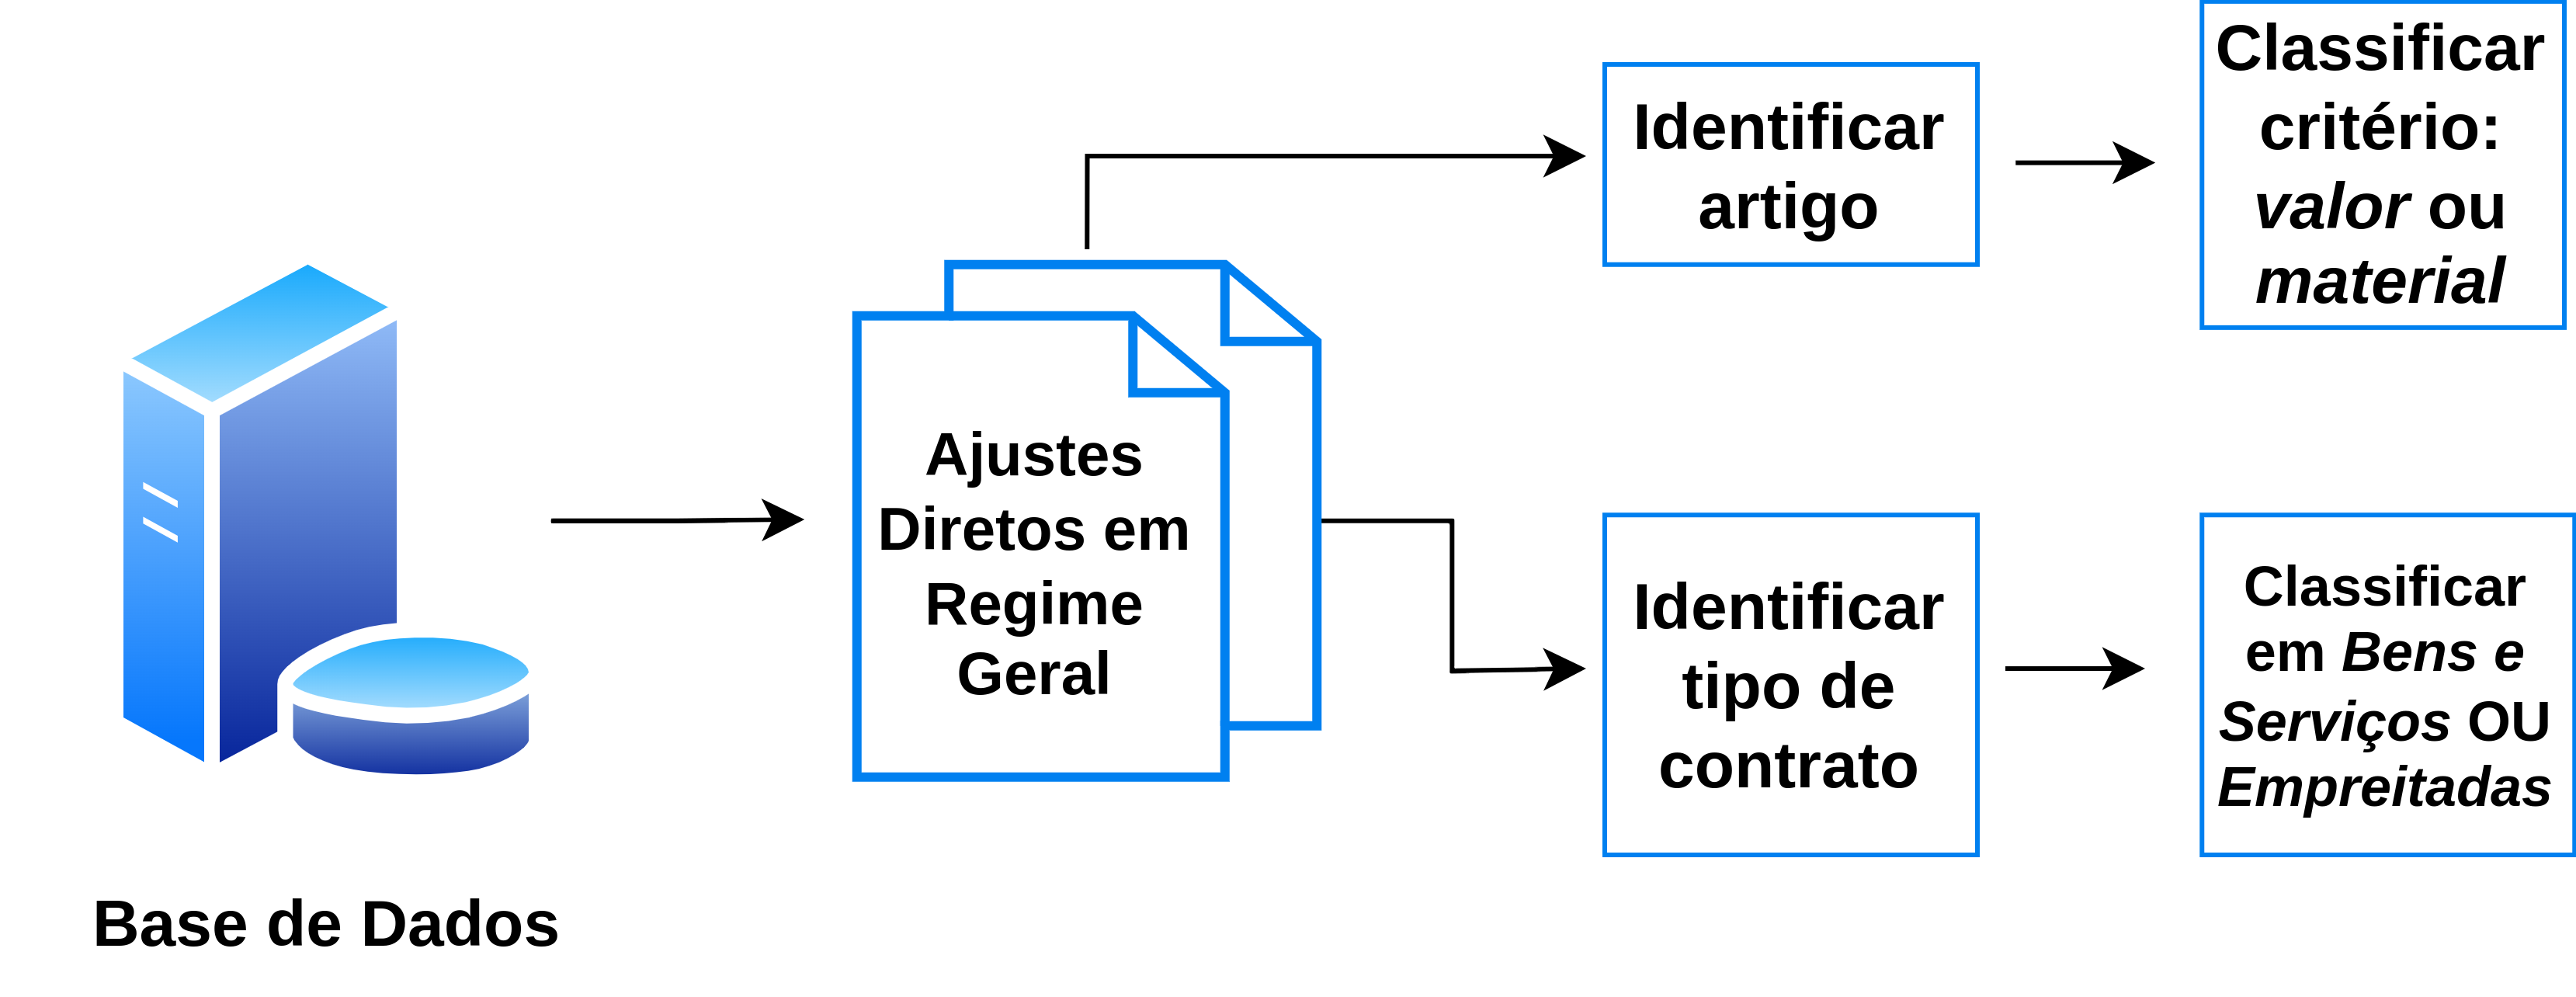
\includegraphics[width=0.9\textwidth]{imagens/rf1.png}
	\caption{Ilustração do processo de classificação de ajustes diretos em regime geral}
	\label{}
\end{figure}

%\begin{lstlisting}[
%	language=SQL,
%	showspaces=false,
%	showstringspaces=false,
%	basicstyle=\ttfamily,
%	numbers=left,
%	numberstyle=\tiny,
%	commentstyle=\color{gray}, frame = single,	autogobble=true,
%	postbreak=\mbox{\textcolor{red}{$\hookrightarrow$}\space},
%	]
%	ALTER TABLE ajustesdiretos
%	ADD COLUMN artigo text;
%	
%	UPDATE ajustesdiretos
%	SET artigo = TRIM(SUBSTRING(fundamentacao 
%			FROM 1 FOR POSITION('º' IN fundamentacao)));
%\end{lstlisting}

%\begin{lstlisting}[
%	language=SQL,
%	showspaces=false,
%	showstringspaces=false,
%	basicstyle=\ttfamily,
%	numbers=left,
%	numberstyle=\tiny,
%	commentstyle=\color{gray}, frame = single,	autogobble=true,
%	postbreak=\mbox{\textcolor{red}{$\hookrightarrow$}\space},
%	]
%	ALTER TABLE ajustesdiretos
%	ADD COLUMN criterio text;
%	
%	UPDATE ajustesdiretos
%	SET criterio = CASE
%	WHEN artigo = 'Artigo 17.º' OR artigo = 'Artigo 18.º' 
%	OR artigo = 'Artigo 19.º' OR artigo = 'Artigo 20.º' 
%	OR artigo = 'Artigo 21.º' OR artigo = 'Artigo 22.º' 
%	THEN 'valor'
%	
%	ELSE 'material' 
%	END;
%\end{lstlisting}


Concluídas as classificações, quanto à tipologia e fundamentação, é possível identificar todos os contratos que não respeitem os valores apresentados na Tabela \ref{tab:4} a partir da seguinte \textit{query}: 


\begin{lstlisting}[
	language=SQL,
	showspaces=false,
	showstringspaces=false,
	basicstyle=\ttfamily,
	numbers=left,
	numberstyle=\tiny,
	commentstyle=\color{gray}, frame = single,	autogobble=true,
	breaklines=true,
	postbreak=\mbox{\textcolor{red}{$\hookrightarrow$}\space},
	]
	SELECT id
	FROM ajustesdiretos
	WHERE (criterio = 'valor' AND tipocontrato = 'Bens e Servicos' AND preco > 20000) OR (criterio = 'valor' AND tipocontrato = 'Empreitadas' AND preco > 30000);
\end{lstlisting}

Da totalidade de Ajustes Diretos em Regime Geral presentes na base de dados\footnote{Relembra-se que foram celebrados 526860 Ajustes Diretos em Regime Geral entre 01/01/2018 e 01/05/2024.}, 14812(2.8\%) destes foram adjudicados com um valor superior ao permitido por lei. Destes, 12828(2.4\%) dizem respeito a contratos de \textbf{Bens e Serviços} e 1984(0.4\%) a contratos de \textbf{Empreitadas}.


\begin{figure}[H]
	\centering
	\begin{minipage}{.45\linewidth}
		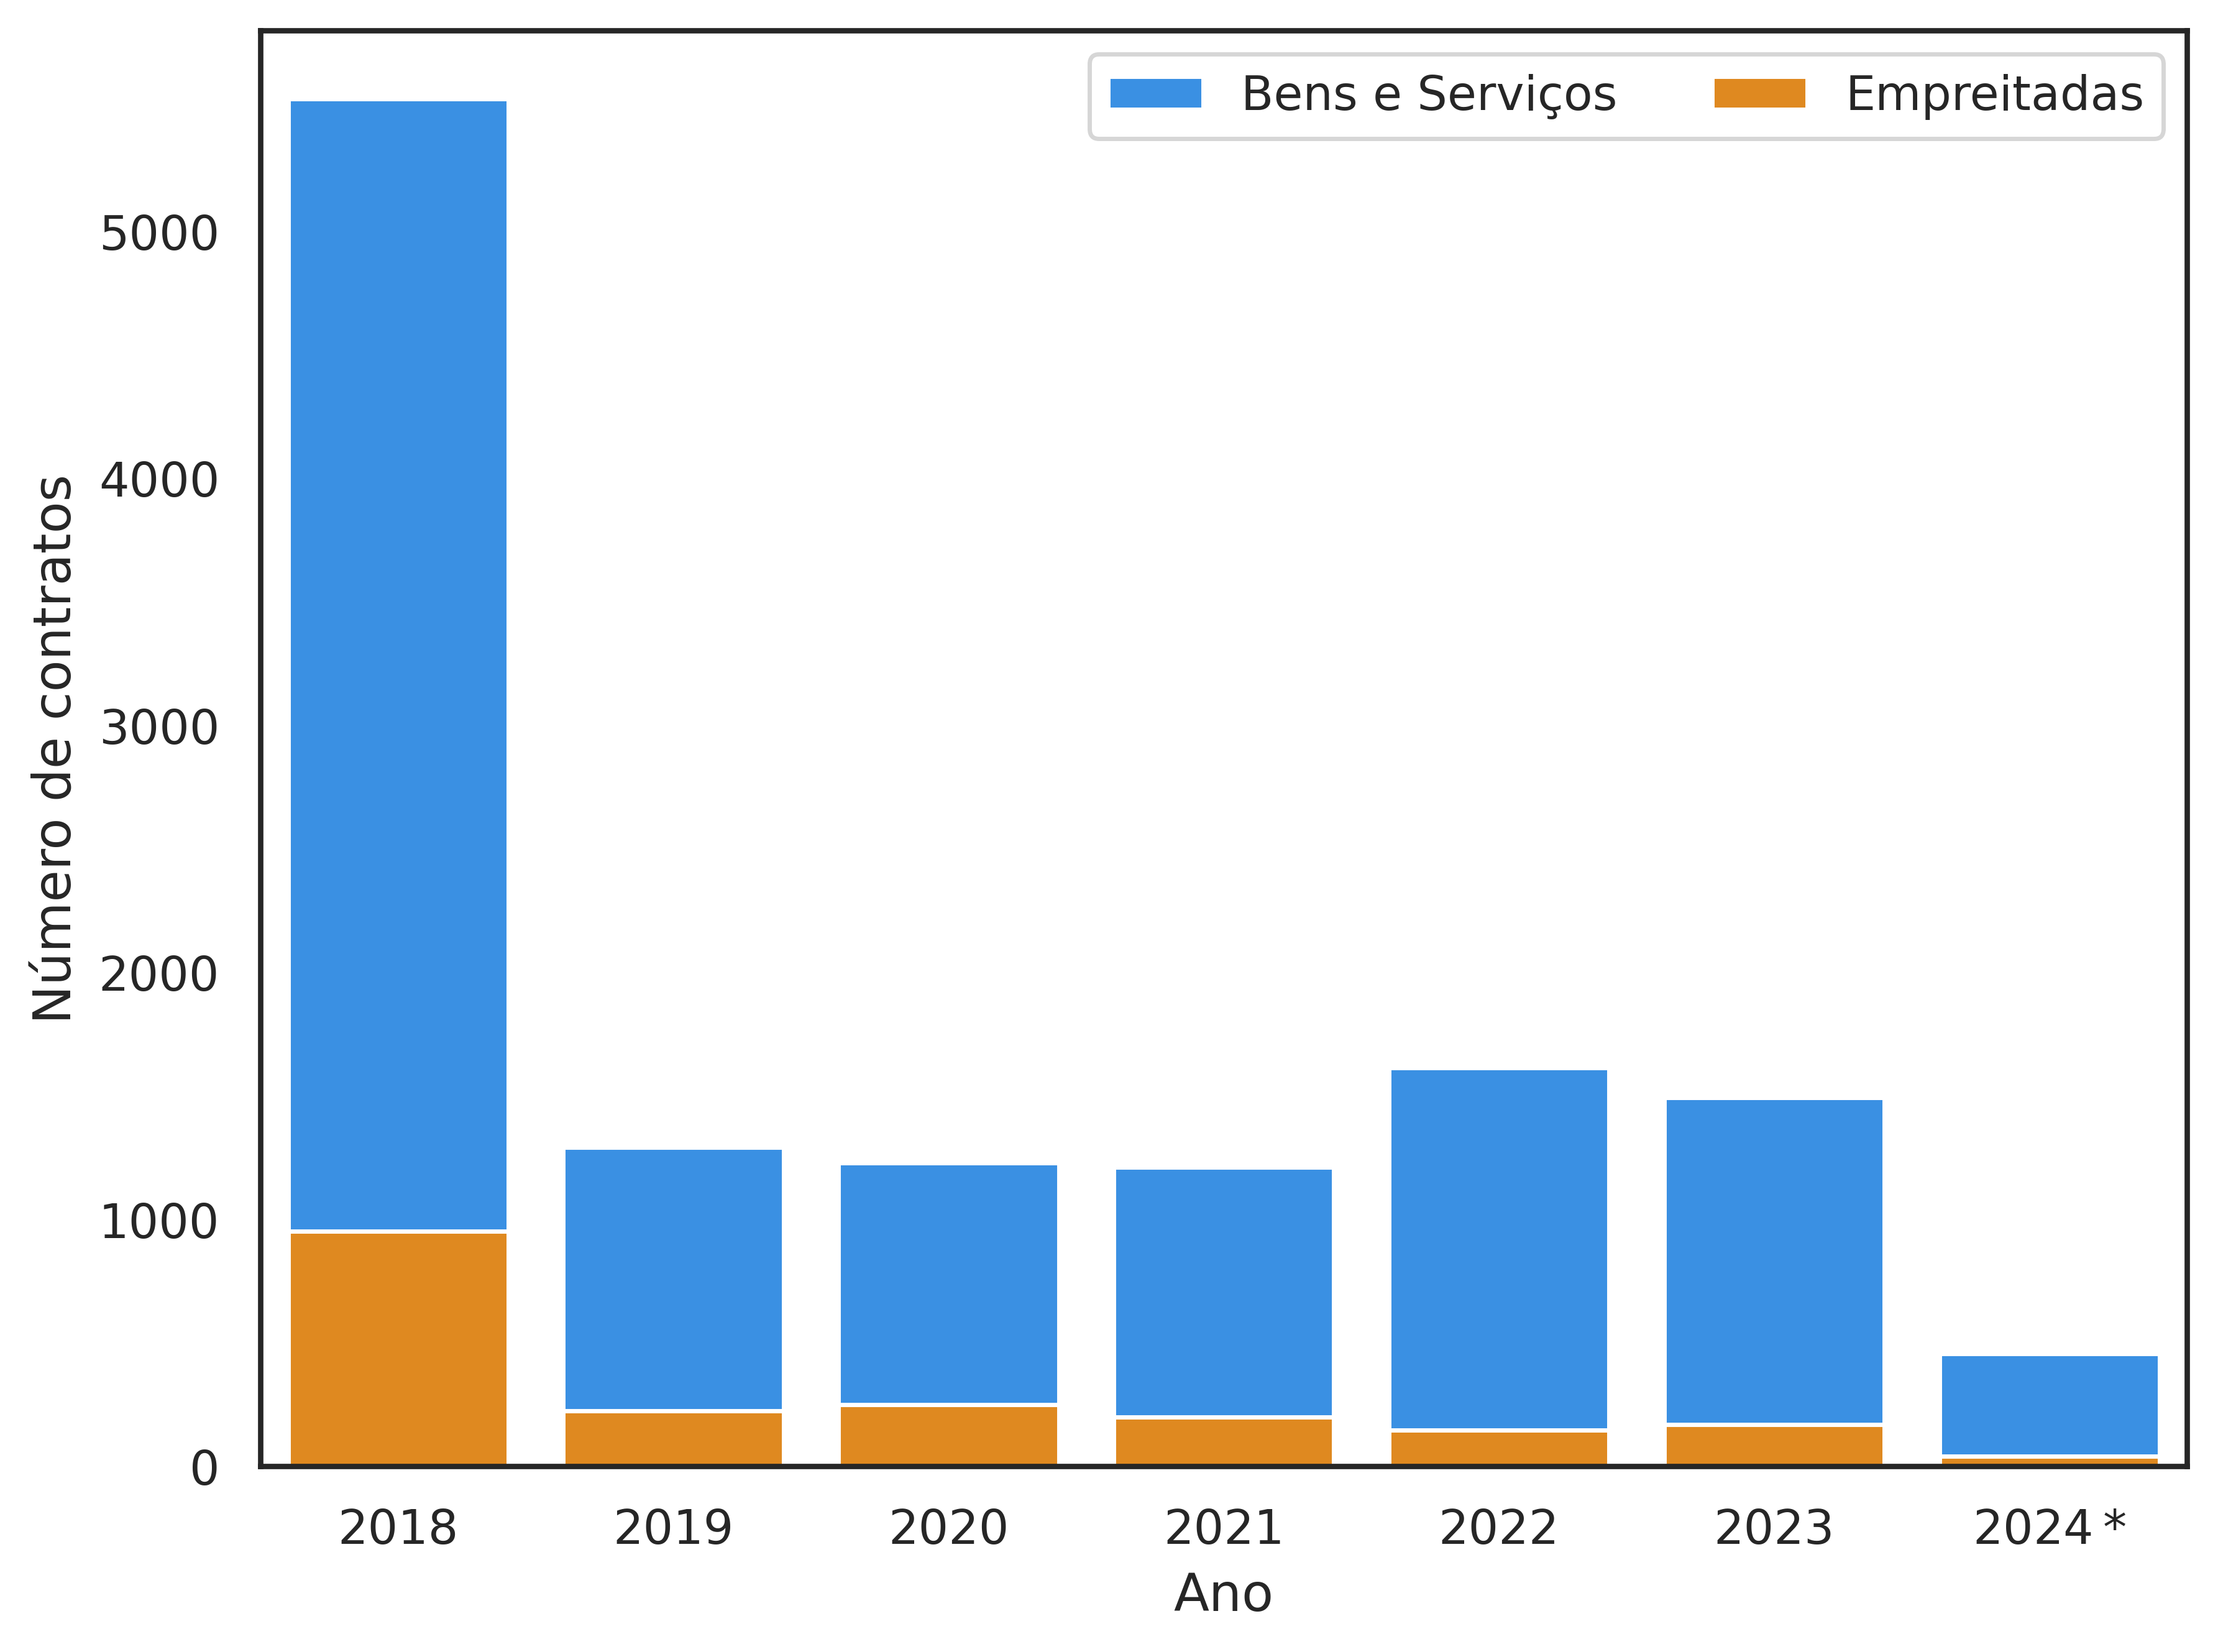
\includegraphics[width=\linewidth]{imagens/rf1/dist.png}
		\caption{Distribuição do número de contratos em inconformidade com o CCP.}
		
	\end{minipage}
	\hfill
	\begin{minipage}{.5\linewidth}
		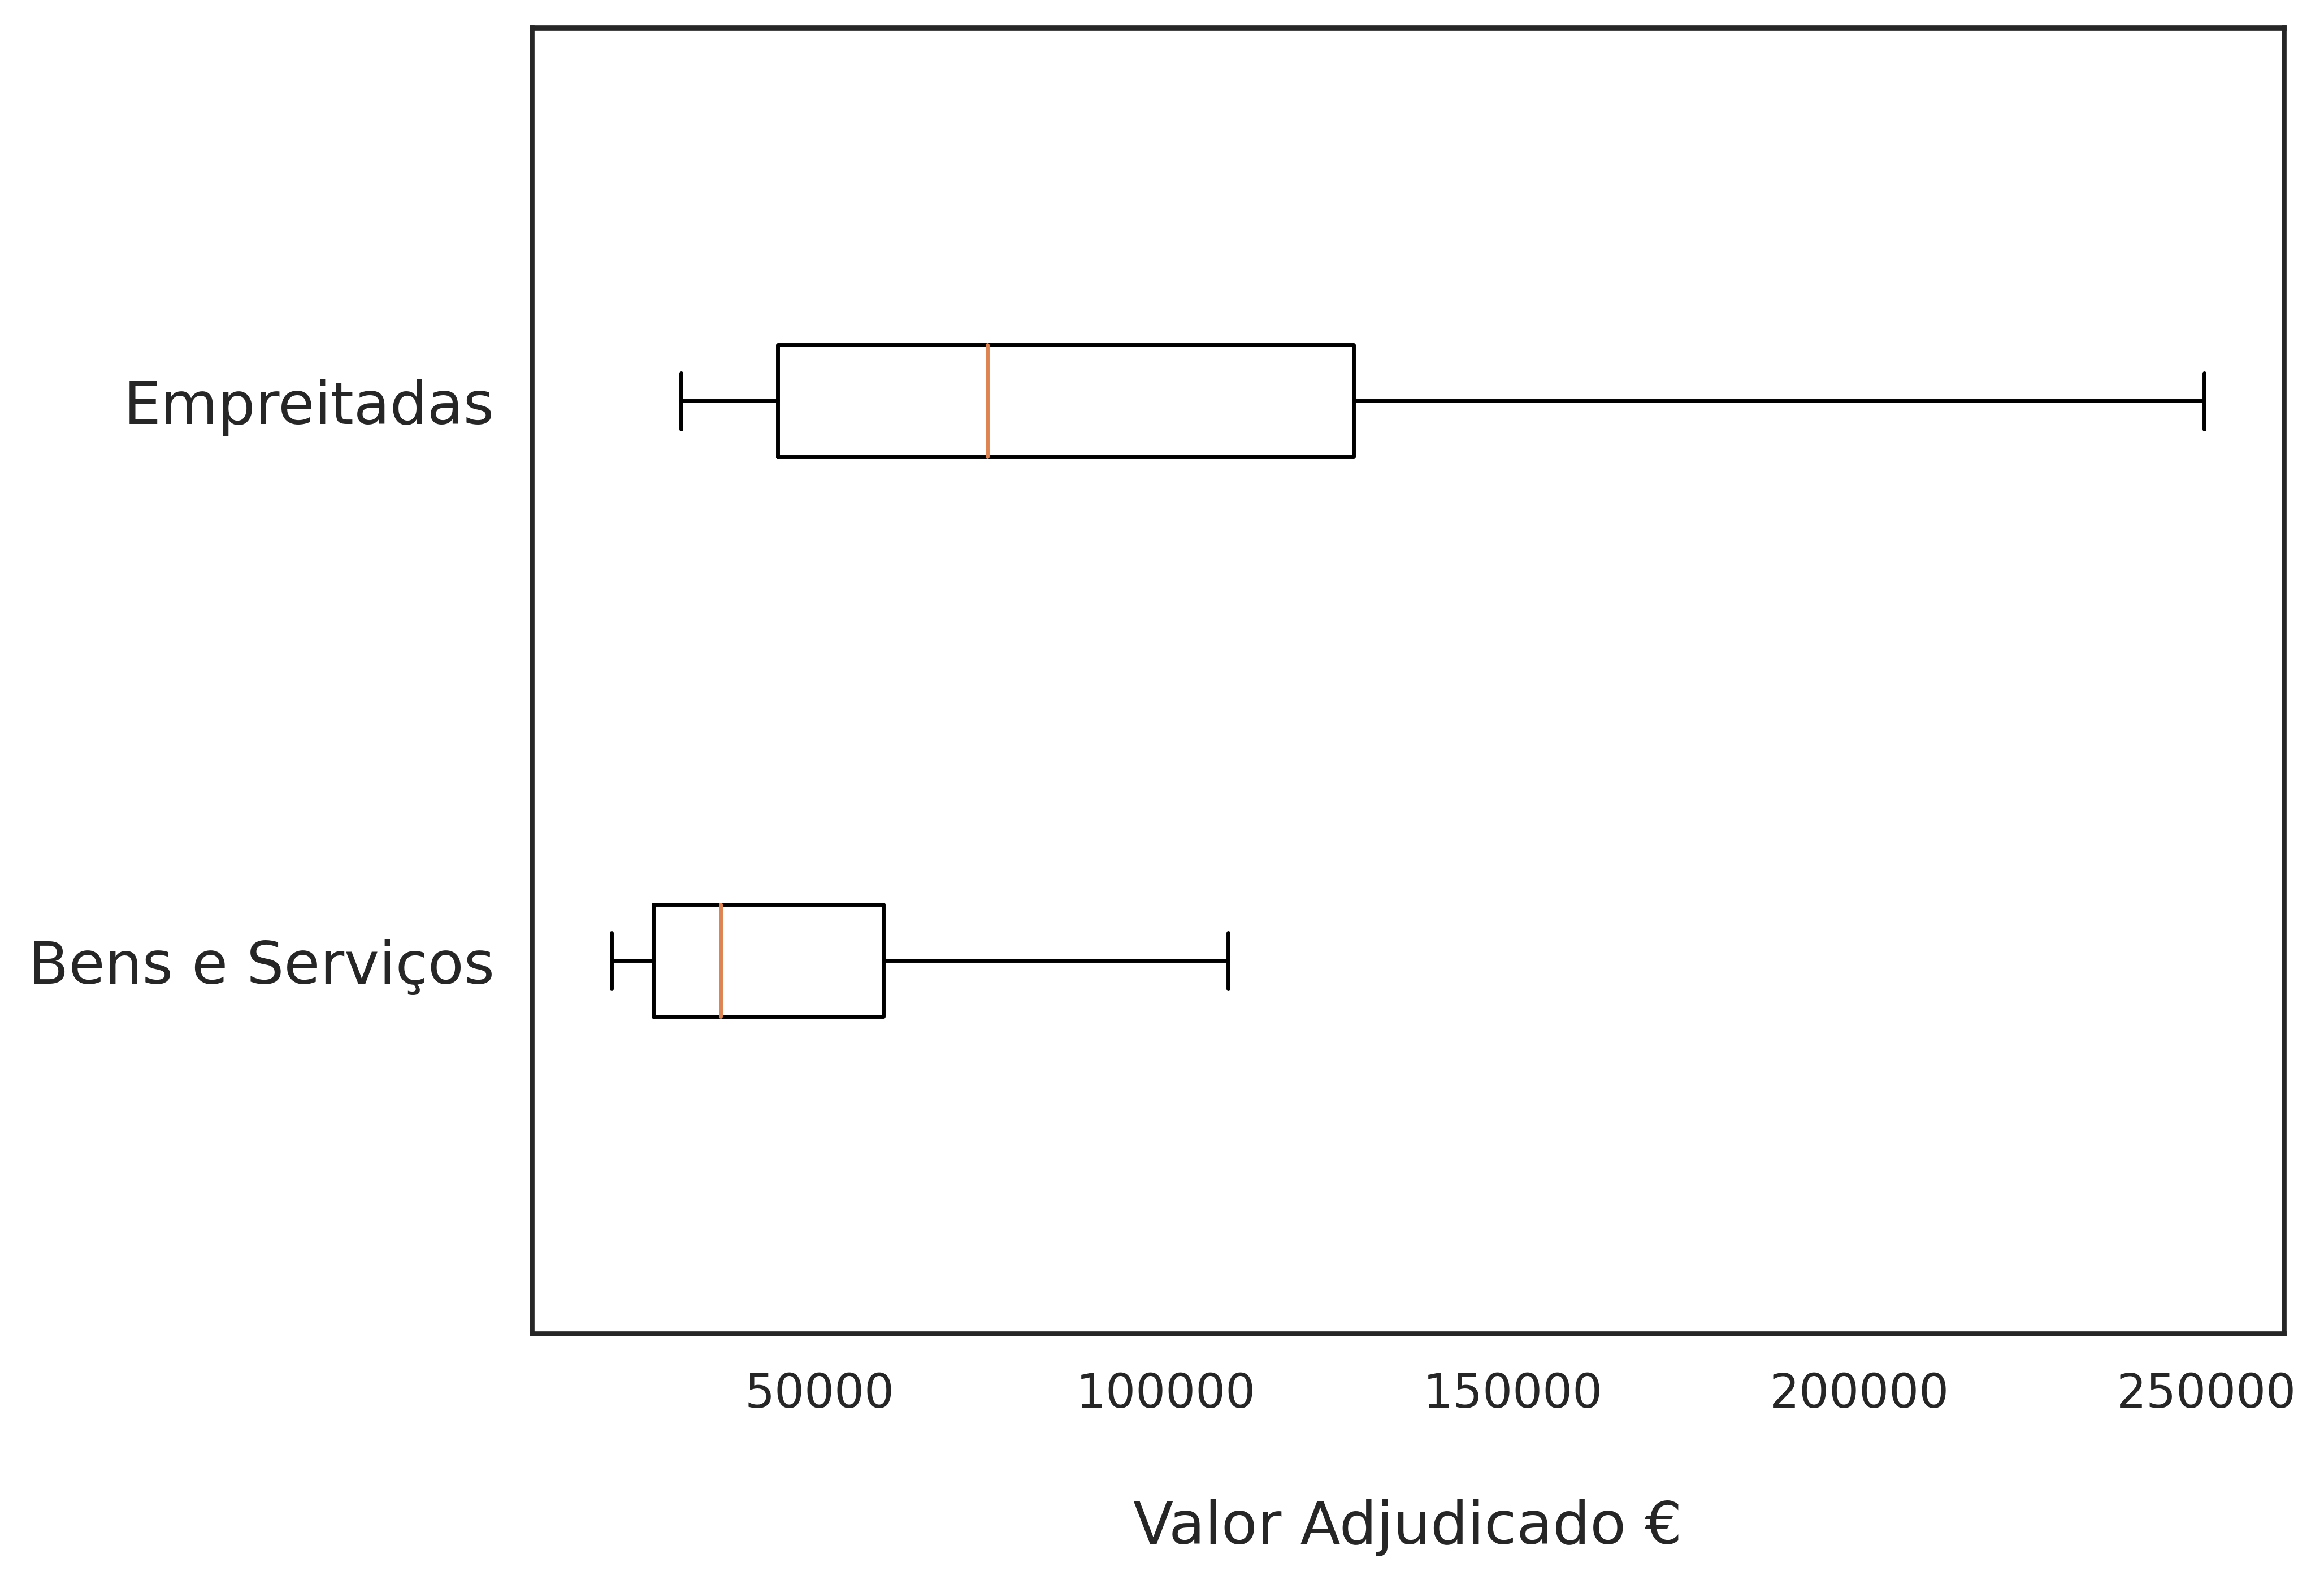
\includegraphics[width=\linewidth]{imagens/rf1/boxplot.png}
		\caption{Boxplot dos valores contratuais para os contratos em inconformidade com a lei.}
		\label{fig:boxaj}
	\end{minipage}
\end{figure}

Na Figura \ref{fig:boxaj} pode observar-se a dispersão dos valores contratuais para todos os ajustes diretos em inconformidade, de acordo com a tipologia de contrato.

Para \textbf{Obras}, 50\% dos contratos em inconformidade (992) foram celebrados com um valor adjudicado, sensivelmente, superior a 75.000,00 €\footnote{Valor da mediana.}, o que equivale a $2.5$ vezes o valor máximo permitido por lei. Por sua vez, o maior valor contratual, de entre todos os ajustes diretos, e que diz respeito a obras numa linha de caminhos de ferro, foi contratualizado por um valor 170 vezes superior ao limite estipulado por lei, cifrando-se nos 5.095.000,00 €.

No caso de \textbf{Bens e Serviços}, existem 50\% de contratos em inconformidade (6414) com um valor adjudicado superior a 35.700,00 €, o que equivale a $1.8$ vezes o valor máximo permitido por lei. O valor máximo contratual para esta tipologia de contrato diz respeito à eletrificação de uma linha férrea, com um valor adjudicado de 3.815.199,75€, $127$ vezes superior ao valor máximo permitido.


Na Figura \ref{fig:maincpvsaj} é possível constatar que a principal divisão de CPV, onde se regista a celebração de contratos em inconformidade, é na divisão da construção civil (45), seguido de serviços empresariais (79), serviços de arquitetura, construção, engenharia e inspeção (71) e, por fim, aquisição de equipamentos médicos (33).

\begin{figure}[H]
	\centering
	
\includegraphics[width=\textwidth]{imagens/rf1/maincpvs.png}
	\caption{Principais divisões de CPV com maior número, e respetiva percentagem, de contratos em inconformidade.}
	\label{fig:maincpvsaj}
\end{figure}


Na Tabela \ref{tab:rf1} é possível observar que existem entidades, cujo nome não é divulgado por motivos de confidencialidade, com um elevado número de contratos celebrados em inconformidade com o CCP. 

%\begin{table}[H]
%	\centering
%	\renewcommand{\arraystretch}{1.15}
%	\setlength{\tabcolsep}{15pt}
%	\resizebox{\textwidth}{!}{%
%		\begin{tabular}{lc}
%			\hline
%			\multicolumn{1}{c}{\textbf{Entidade Adjudicante}}                                           & \textbf{Número de Contratos} \\ \hline
%			Infraestruturas de Portugal, S. A.                                                          & 377                          \\
%			Hospital de Santo Espírito da Ilha Terceira, E. P. E. R.                                    & 329                          \\
%			Município de Ponta Delgada                                                                  & 204                          \\
%			Instituto Português de Oncologia do Porto Francisco Gentil, E. P. E.                        & 203                          \\ \hline
%			\multicolumn{1}{c}{\textbf{Entidade Vencedora}}                                             & \textbf{Número de Contratos} \\ \hline
%			Meo - Serviços de Comunicações e Multimédia S.A                                             & 165                          \\
%			Urbhorta - Construção, Gestão e Exploração de Projectos de Desenvolvimento Empresarial, EEM & 53                           \\
%			Sotermáquinas-Sociedade Terceirense de Máquinas e Acessórios S.A                            & 53                          
%		\end{tabular}%
%	}
%	\caption{Entidades, adjudicantes e vencedoras, com maior número de ajustes diretos celebrados em inconformidade com o CCP}
%\end{table}



\begin{table}[H]
	\centering
	\renewcommand{\arraystretch}{1.1}
	\setlength{\tabcolsep}{35pt}
	%\resizebox{\textwidth}{!}{%
		\begin{tabular}{lc}
			\hline
			\textbf{Entidade Adjudicante} & \multicolumn{1}{r}{\textbf{Número de Contratos}} \\ \hline
			Empresa A                     & 377                                              \\
			Empresa B                     & 329                                              \\
			Empresa C                     & 204                                              \\
			Empresa D                     & 203                                              \\ \hline
			\textbf{Entidade Vencedora}   & \textbf{Número de Contratos}                     \\ \hline
			Empresa E                     & 165                                              \\
			Empresa F                     & 53                                               \\
			Empresa G                     & 53                                              
		\end{tabular}%
	%}
	\caption{Entidades, adjudicantes e vencedoras, com maior número de ajustes diretos celebrados em inconformidade com o CCP.}
	\label{tab:rf1}
\end{table}


% ADCIONAR À SECÇÃO DOS ANEXOS
%\begin{figure}[H]
%	\centering
%	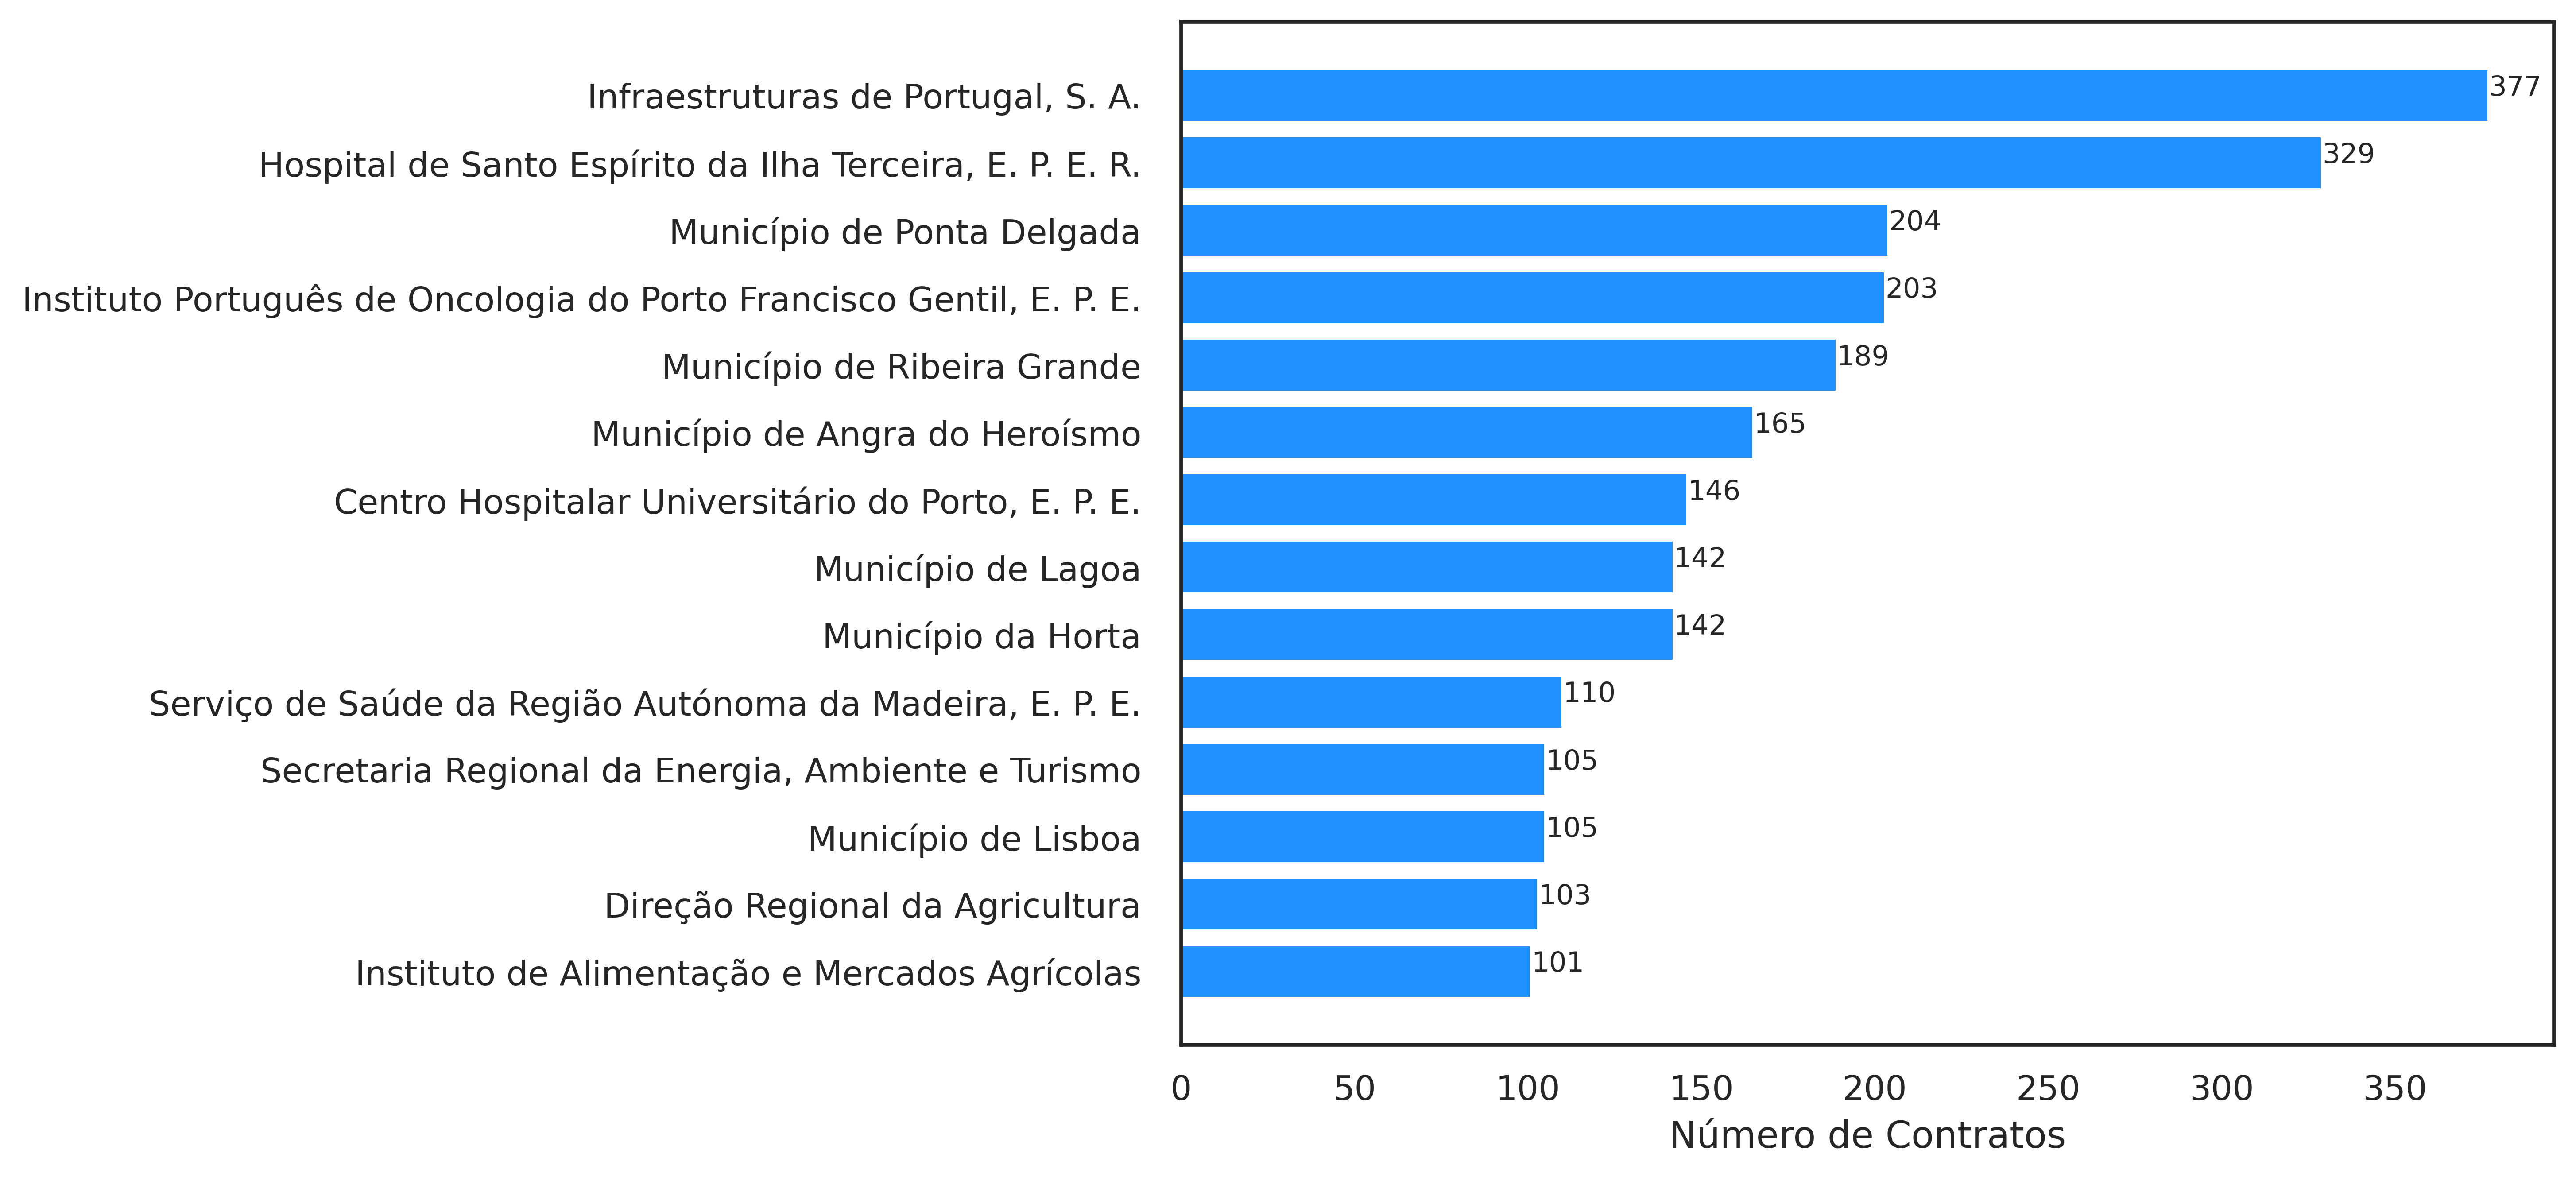
\includegraphics[width=\textwidth]{imagens/rf1/adjudicantes.png}
%	\caption{Entidades Adjudicantes com maior número de ajustes diretos celebrados em inconformidade com o CCP}
%	\label{}
%\end{figure}
%
%
%
%\begin{figure}[H]
%	\centering
%	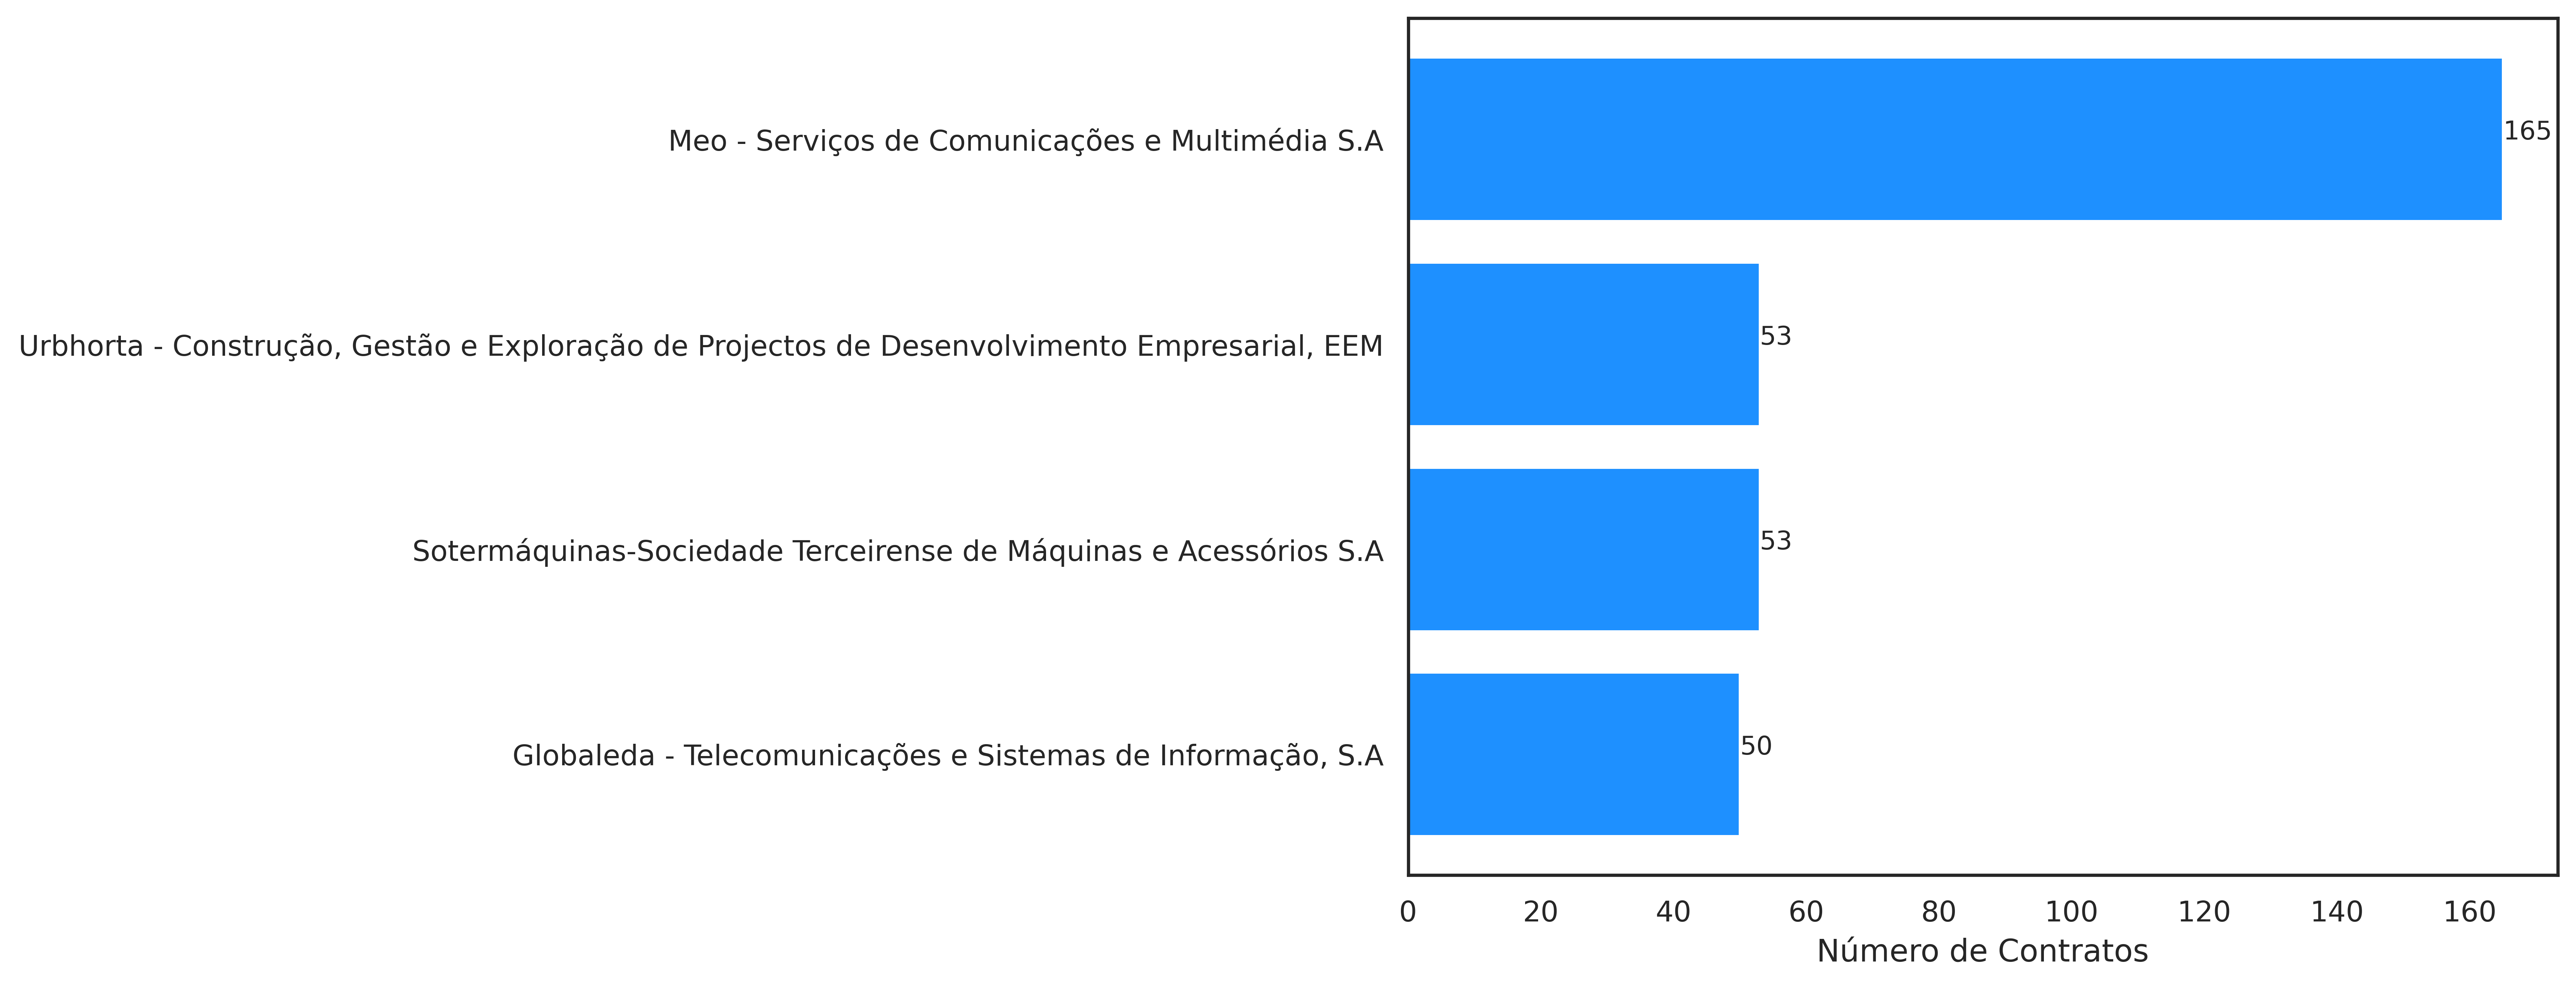
\includegraphics[width=\textwidth]{imagens/rf1/vencedora.png}
%	\caption{Entidades Adjudicantes com maior número de ajustes diretos celebrados em inconformidade com o CCP}
%	\label{}
%\end{figure}



\section{R003: Análise do prazo de apresentação de propostas}

Um factor relevante a considerar na fase da publicitação de um concurso público, é o prazo disponível para que as diferentes entidades interessadas possam apresentar propostas. Uma das flags definidas pela OCDS incide precisamente sobre esta questão\footnote{Short or inadequate notice to bidders to submit expressions of interest or bids. Bid period is less than expected (usually $\leq$2 days). The indicator should be calculated grouping by procurement method used, since the minimum bidding period might vary depending on the method.  It is important to check in local regulations if there is a minimun period.}.

%\Lemma{\cite{spreadsheet1}}
%{}

De acordo com o artigo 135.º do CCP - ver Tabela \ref{table:3} - o prazo mínimo para apresentação de propostas num concurso público para Bens e Serviços não pode ser inferior a 6 dias e, no caso de se tratar de um  contrato de empreitada de obras públicas, inferior a 14 dias. Assim, para a construção desta flag, foi criada uma coluna adicional na tabela \textit{concursos\_publicos} denominada \textbf{tipo\_contrato}, tal como no indicador RF1. Posteriormente, foi construída uma \textit{query} para determinar todos os concursos públicos que não respeitam as condições apresentadas na Tabela \ref{table:3}. \\


\begin{lstlisting}[
	language=SQL,
	showspaces=false,
	showstringspaces=false,
	basicstyle=\ttfamily,
	numbers=left,
	numberstyle=\tiny,
	commentstyle=\color{gray}, frame = single,
	autogobble=true,
	breaklines=true,
	postbreak=\mbox{\textcolor{red}{$\hookrightarrow$}\space},
	]
	SELECT contratos_basegov."id" 
	FROM contratos_basegov
	JOIN concursos_publicos ON contratos_basegov."id" = concursos_publicos."id"
	WHERE (concursos_publicos."tipo_contrato" = 'Empreitadas' AND contratos_basegov."anuncio_proposalDeadline" < 14) 
	OR
	(concursos_publicos."tipo_contrato" = 'Bens e Servicos' AND contratos_basegov."anuncio_proposalDeadline" < 6);
	
\end{lstlisting}


%Foi incluída uma condição adicional na \textit{query} para selecionar os contratos com prazo de apresentação de propostas superior a 0 dias. Esta condição foi imposta pois verificou-se que existiam alguns contratos com prazos negativos. Tendo em conta a dimensão dos valores - sempre superiores a 10, em módulo - inferiu-se que seriam erros de preenchimento aquando da inserção do contrato no Portal BASE porém não foram considerados na construção deste indicador. 

Do total de concursos públicos celebrados\footnote{Relembra-se que o número de concursos públicos celebrados, no período de tempo considerado no Capítulo \ref{ch:variables}, foi de 124422.}, verificou-se a existência de 4698 (3.7\%) contratos em inconformidade com a condição imposta por este indicador, sendo 1787 referentes a \textbf{Bens e Serviços} e 2911 a \textbf{Obras}. É, novamente, na divisão da Construção Civil onde se verifica a existência de um maior incumprimento do prazo mínimo de dias para apresentação de propostas, representando cerca de 60\% (2871) da totalidade dos contratos em inconformidade. 

De acordo com a Figura \ref{fig:minday}, constata-se que 50\% dos contratos inconformes (1455) da tipologia \textbf{Obras} dispõe, no máximo, de 9 dias para apresentar propostas. Dos 2911 contratos em inconformidade, verificou-se a existência de 32 com apenas um dia para a apresentação de propostas. 

Dos 1787 contratos referentes a \textbf{Bens e Serviços},
verificou-se a existência de 173 com apenas um dia para a aprensentação de propostas. 
 

\begin{figure}[H]
	\centering
	\begin{minipage}{.48\linewidth}
		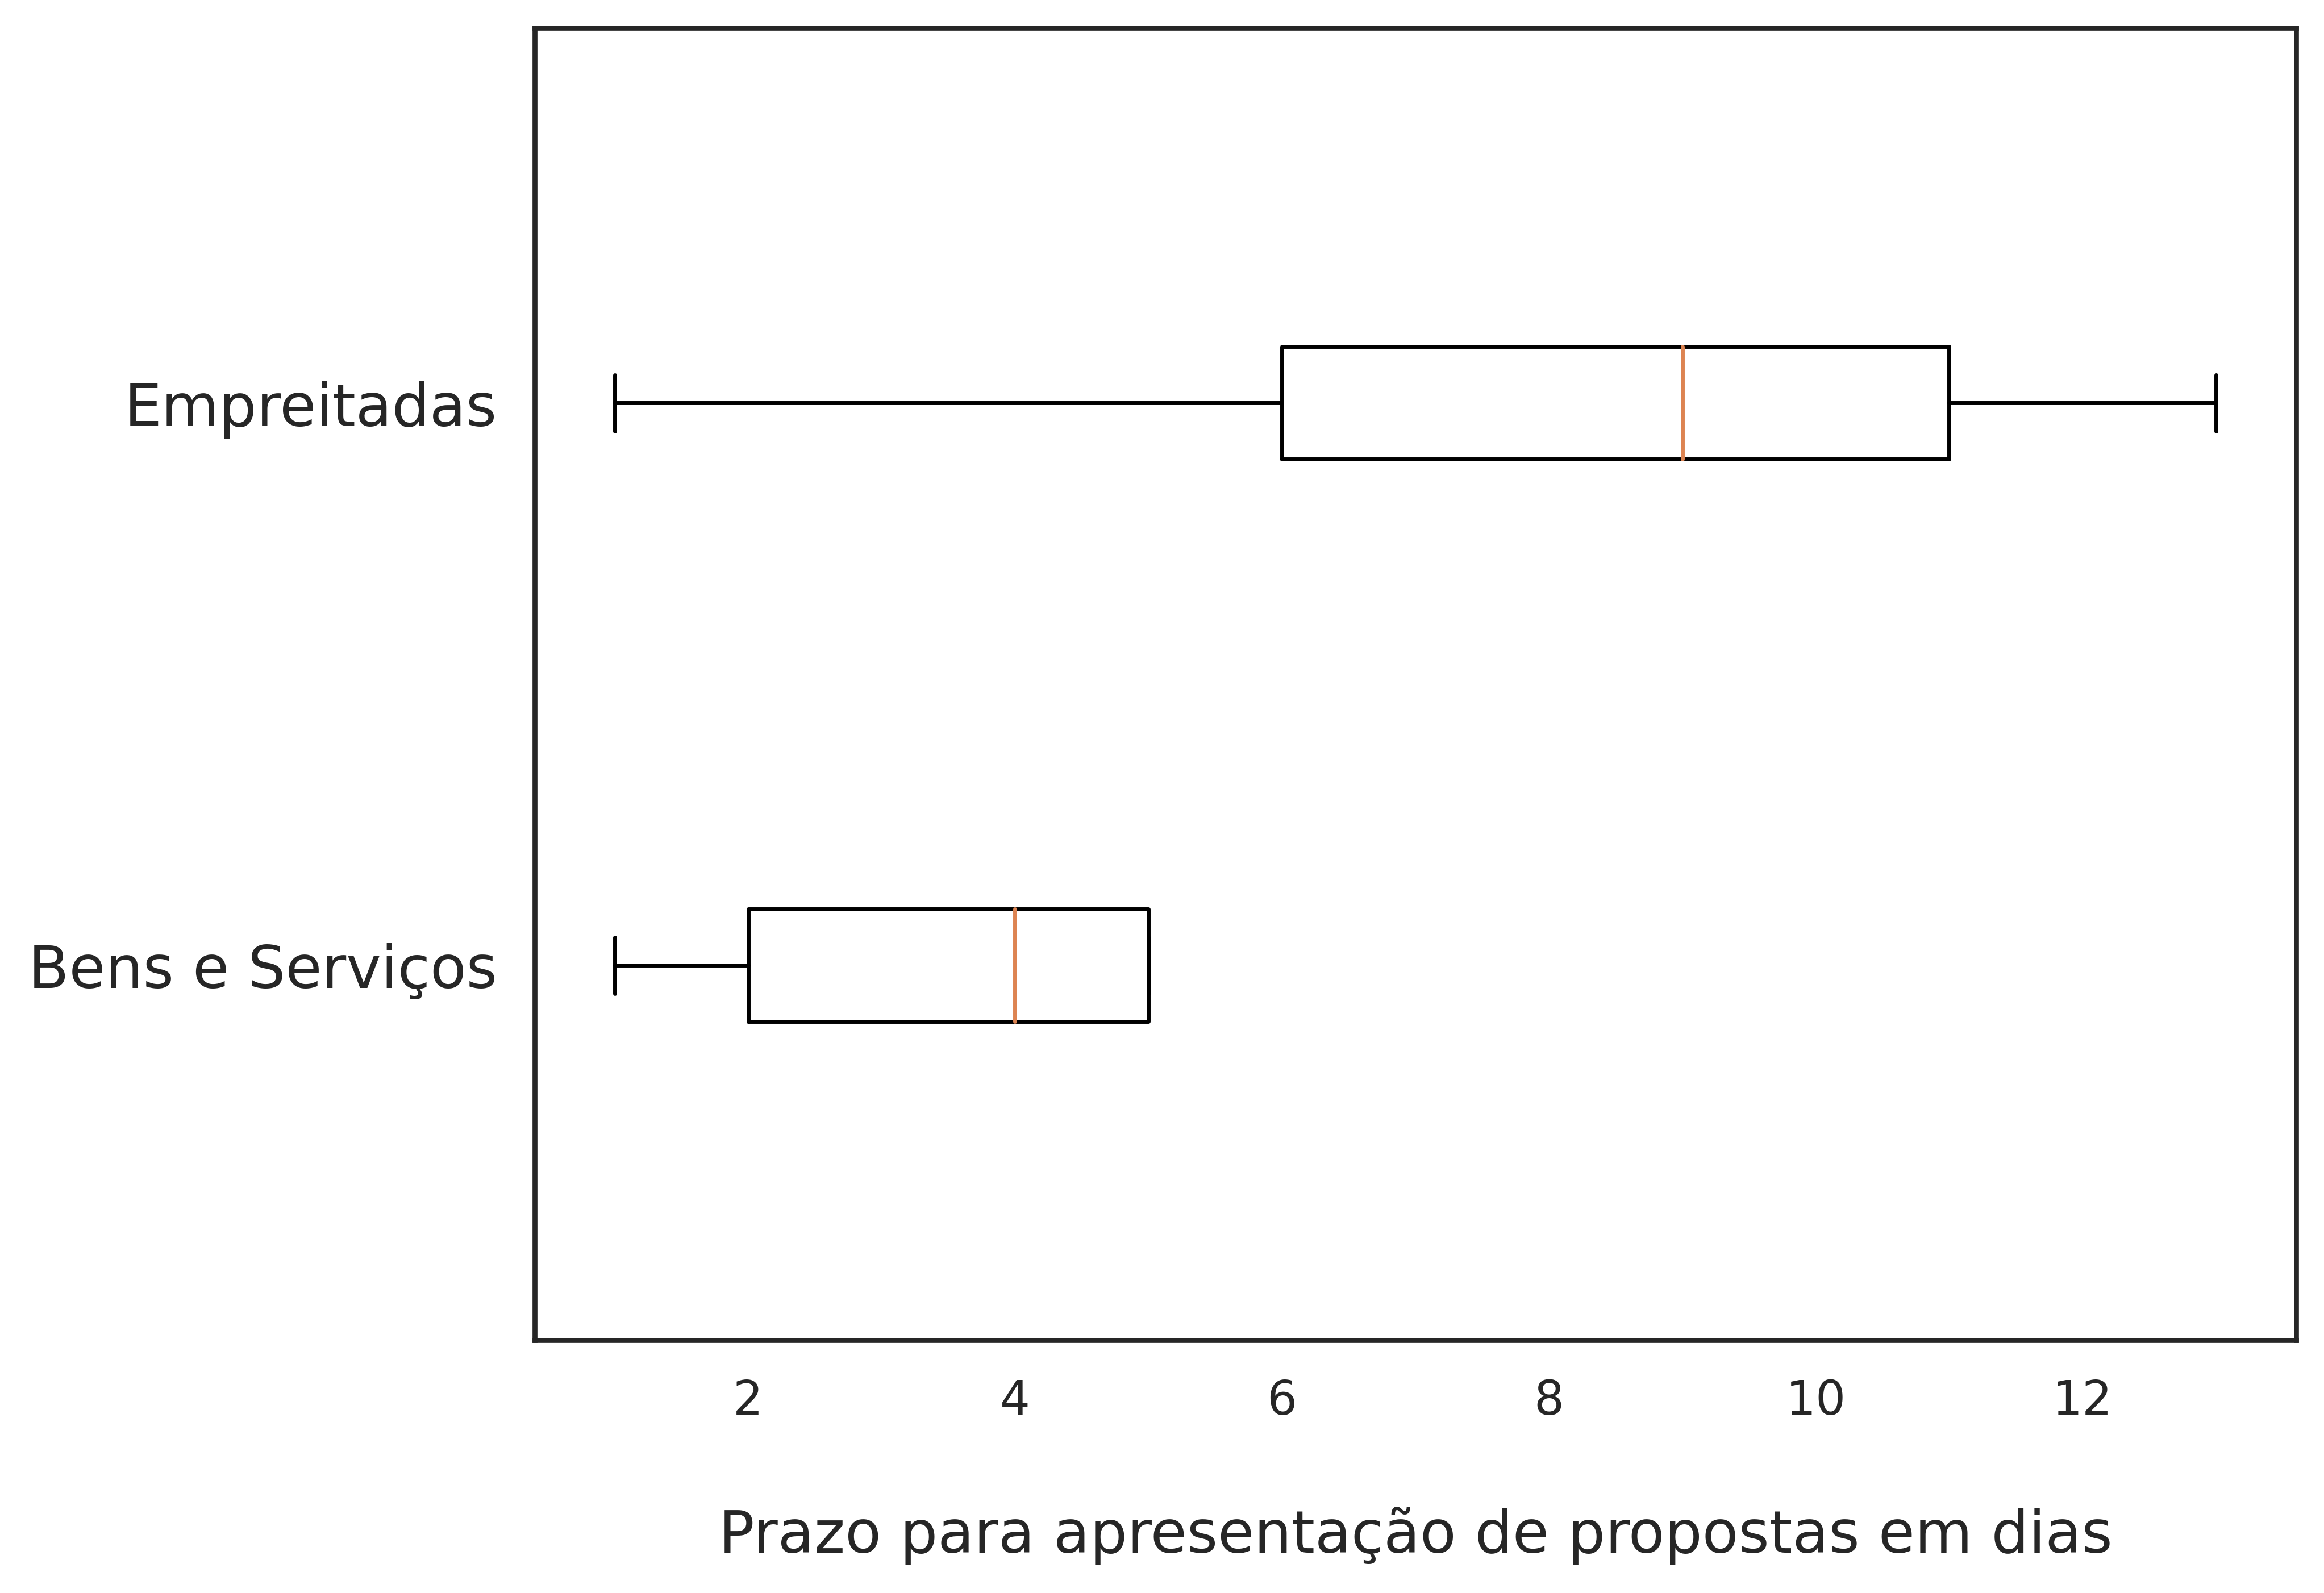
\includegraphics[width=\linewidth]{imagens/r003/boxplot_prazos.png}
		\caption{Distribuição do prazo de apresentação das propostas, em dias, para as duas tipologias de contratos.}
		\label{fig:minday}
	\end{minipage}
	\hfill
	\begin{minipage}{.48\linewidth}
		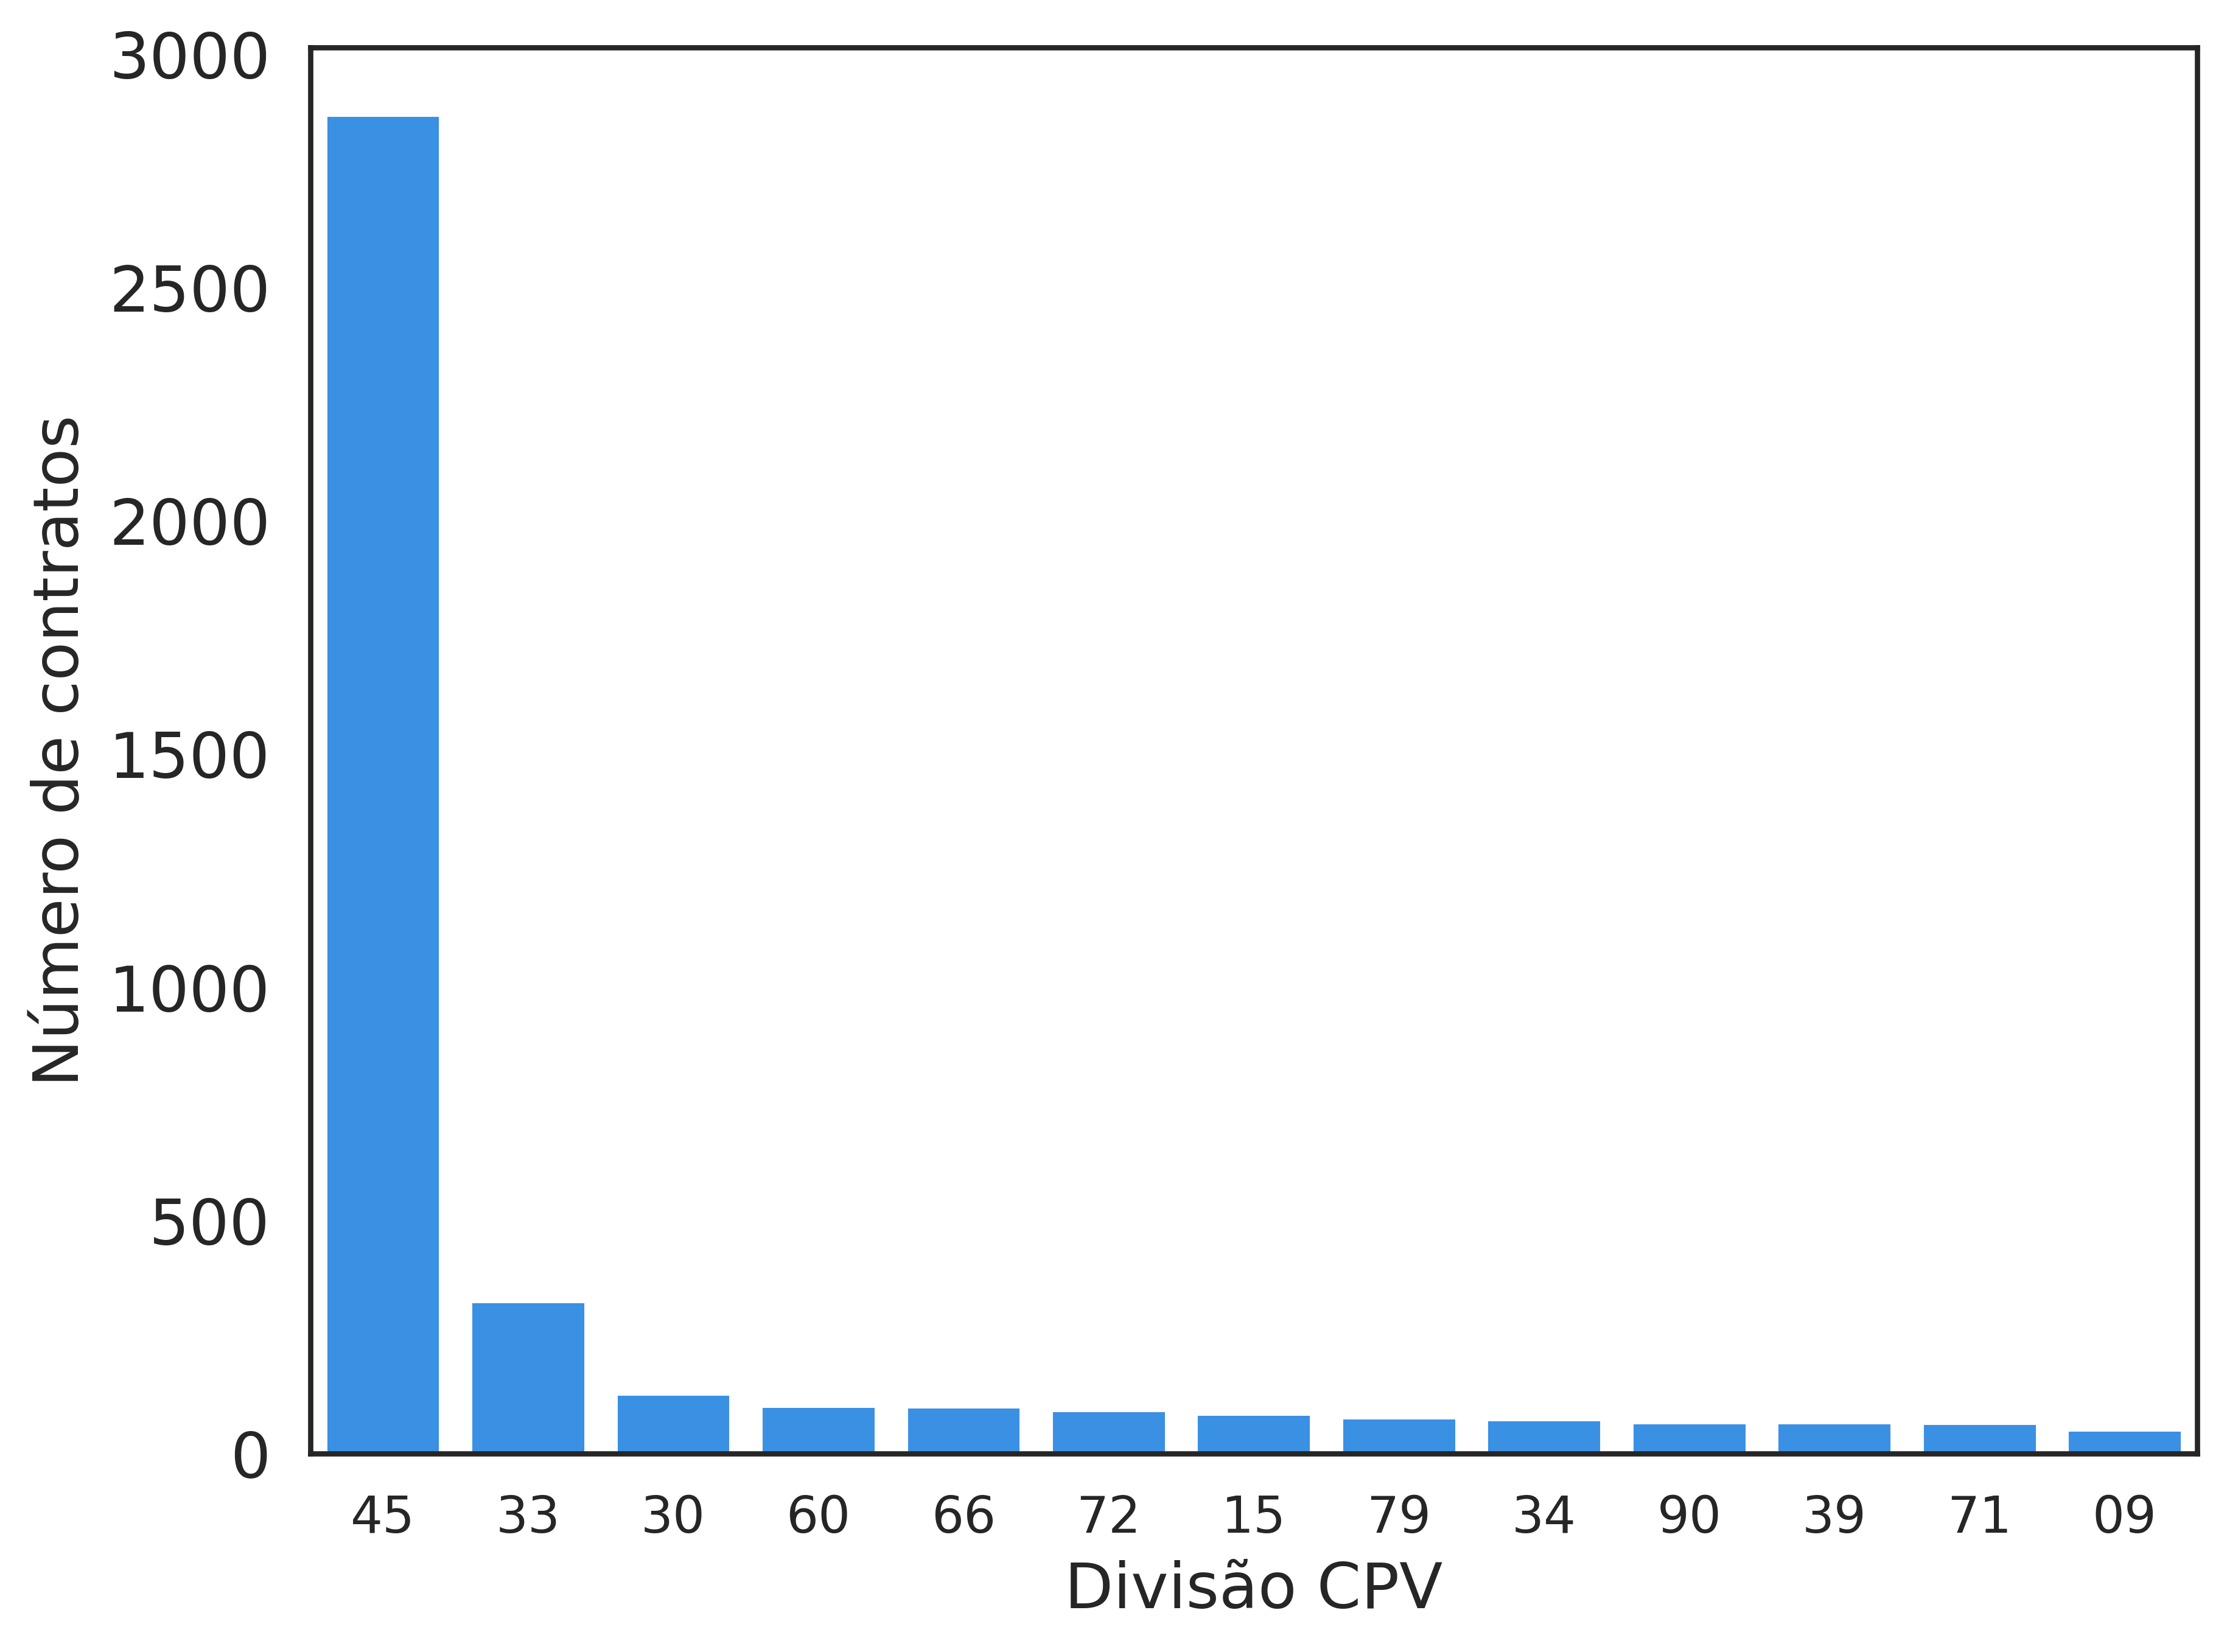
\includegraphics[width=\linewidth]{imagens/r003/main_cpvs.png}
		\caption{Principais divisões de CPV com maior número de contratos em inconformidade.}
		
	\end{minipage}
\end{figure}













\section{R017: Análise do preço contratual, por grupo de CPV}


A construção deste indicador teve como objectivo verificar se o preço contratual de um determinado contrato se encontrava dentro de um limite expectável, consoante o \hyperref[sec:cepeves]{grupo\footnote{Relembra-se que o grupo do CPV consiste na caracterização de um contrato a partir dos primeiros três dígitos deste número.} do CPV} do mesmo\footnote{The difference between an item value and its expected value is above a threshold.}. Para tal, foi utilizada a tabela auxiliar da base de dados, \textit{precoc\_stat}. Para cada um dos 302 grupos do CPV foram calculados os indicadores estatísticos, preço total adjudicado por grupo e respetivas extremidades, para a deteção de outliers.

Na Tabela \ref{tab:precocstat} encontra-se, a título de exemplo, umas das linhas da tabela \textit{precoc\_stat} para o grupo 157 do CPV, referente a contratos de aquisição de alimentos para animais. Foram celebrados 699 contratos para esta divisão, adjudicados por um valor total de 16.807.688,00€. O valor médio por contrato rondou os 24.045,30€, sendo que 50\% deles foram celebrados com um valor inferior a 12.750,00€. A constante de Medcouple permite aferir que a distribuição de valores é assimétrica à direita e, para qualquer contrato cujo valor adjudicado seja inferior a 2121,30€ ou superior a 156.268,30€, é sinalizado.

\begin{table}[H]
	\centering
	\renewcommand{\arraystretch}{1.4}
	\resizebox{\textwidth}{!}{%
	\begin{tabular}{cccccccccccccc}
		\hline
		\textbf{cpv} & \textbf{preco\_total} & \textbf{count} & \textbf{mean} & \textbf{std} & \textbf{min} & \textbf{q1} & \textbf{q2} & \textbf{q3} & \textbf{max} & \textbf{iqr} & \textbf{mc\_const} & \textbf{lower\_fence} & \textbf{upper\_fence} \\ \hline
		157          & 16.807.688,00€        & 699            & 24.045,30€    & 40.901,61€   & 45.5         & 5890,52€    & 12.750,00€  & 25.000,00€  & 521.364,10€  & 19.109,50€   & 0.51               & 2121,30€              & 156268,30€            \\ \hline
	\end{tabular}%
	}
	\caption{Exemplo de uma linha da tabela \textit{precoc\_stat} para concursos públicos referentes a aquisição de alimentos para animais.}
	\label{tab:precocstat}	
\end{table}




O desenvolvimento deste indicador agregou os contratos, por grupo do CPV, com o objetivo de se conseguir um maior nível de granularidade. Ao construir esta tabela, constatou-se a existência de 6111 contratos com preços contratuais negativos ou nulos. Estes valores foram desconsiderados para o cálculo dos indicadores estatísticos, na determinação da constante de Medcouple e das extremidades superior e inferior do boxplot. 

Aplicando este indicador ao conjunto de concursos públicos, verificou-se a presença de $N_{Total} = 27261$ contratos inconformes, o que equivale a 21\% da totalidade concursos públicos.  

\begin{figure}[H]
	\centering
	\begin{minipage}{.48\linewidth}
		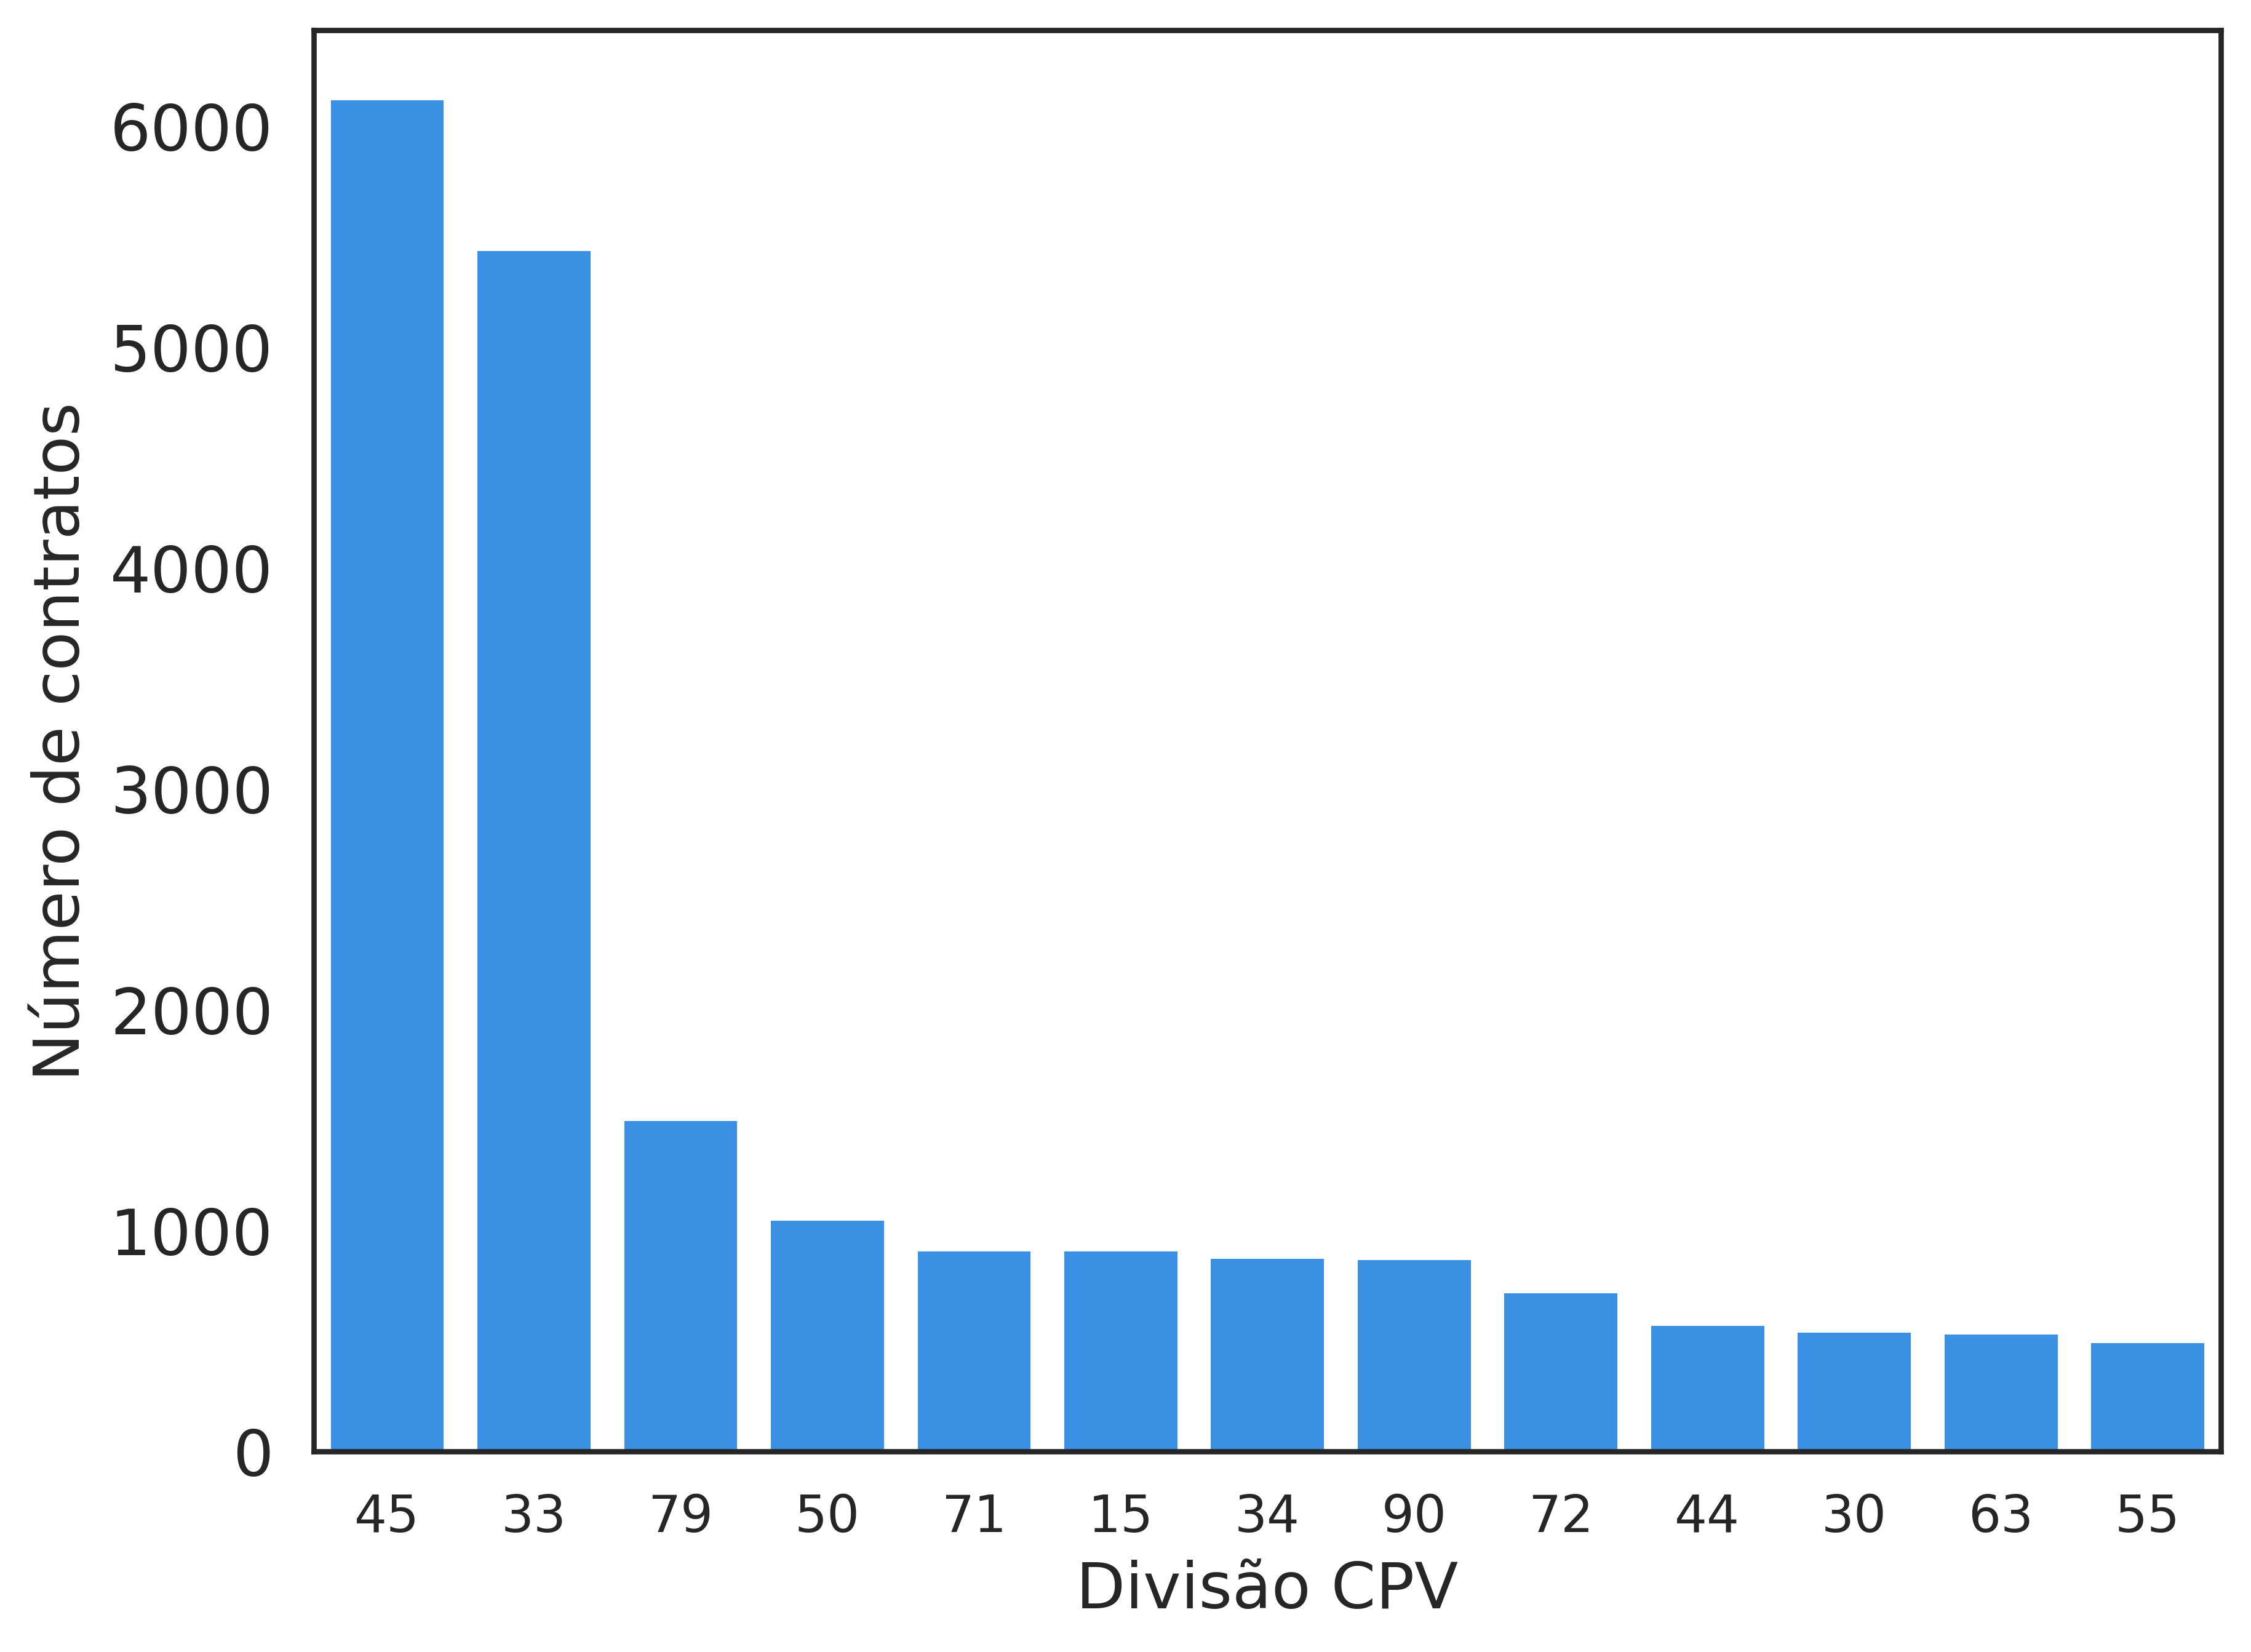
\includegraphics[width=\linewidth]{imagens/r017/cpvdiv.png}
		\caption{Divisões de CPV com maior número de contratos em inconformidade.}
	\end{minipage}
	\hfill
	\begin{minipage}{.49\linewidth}
		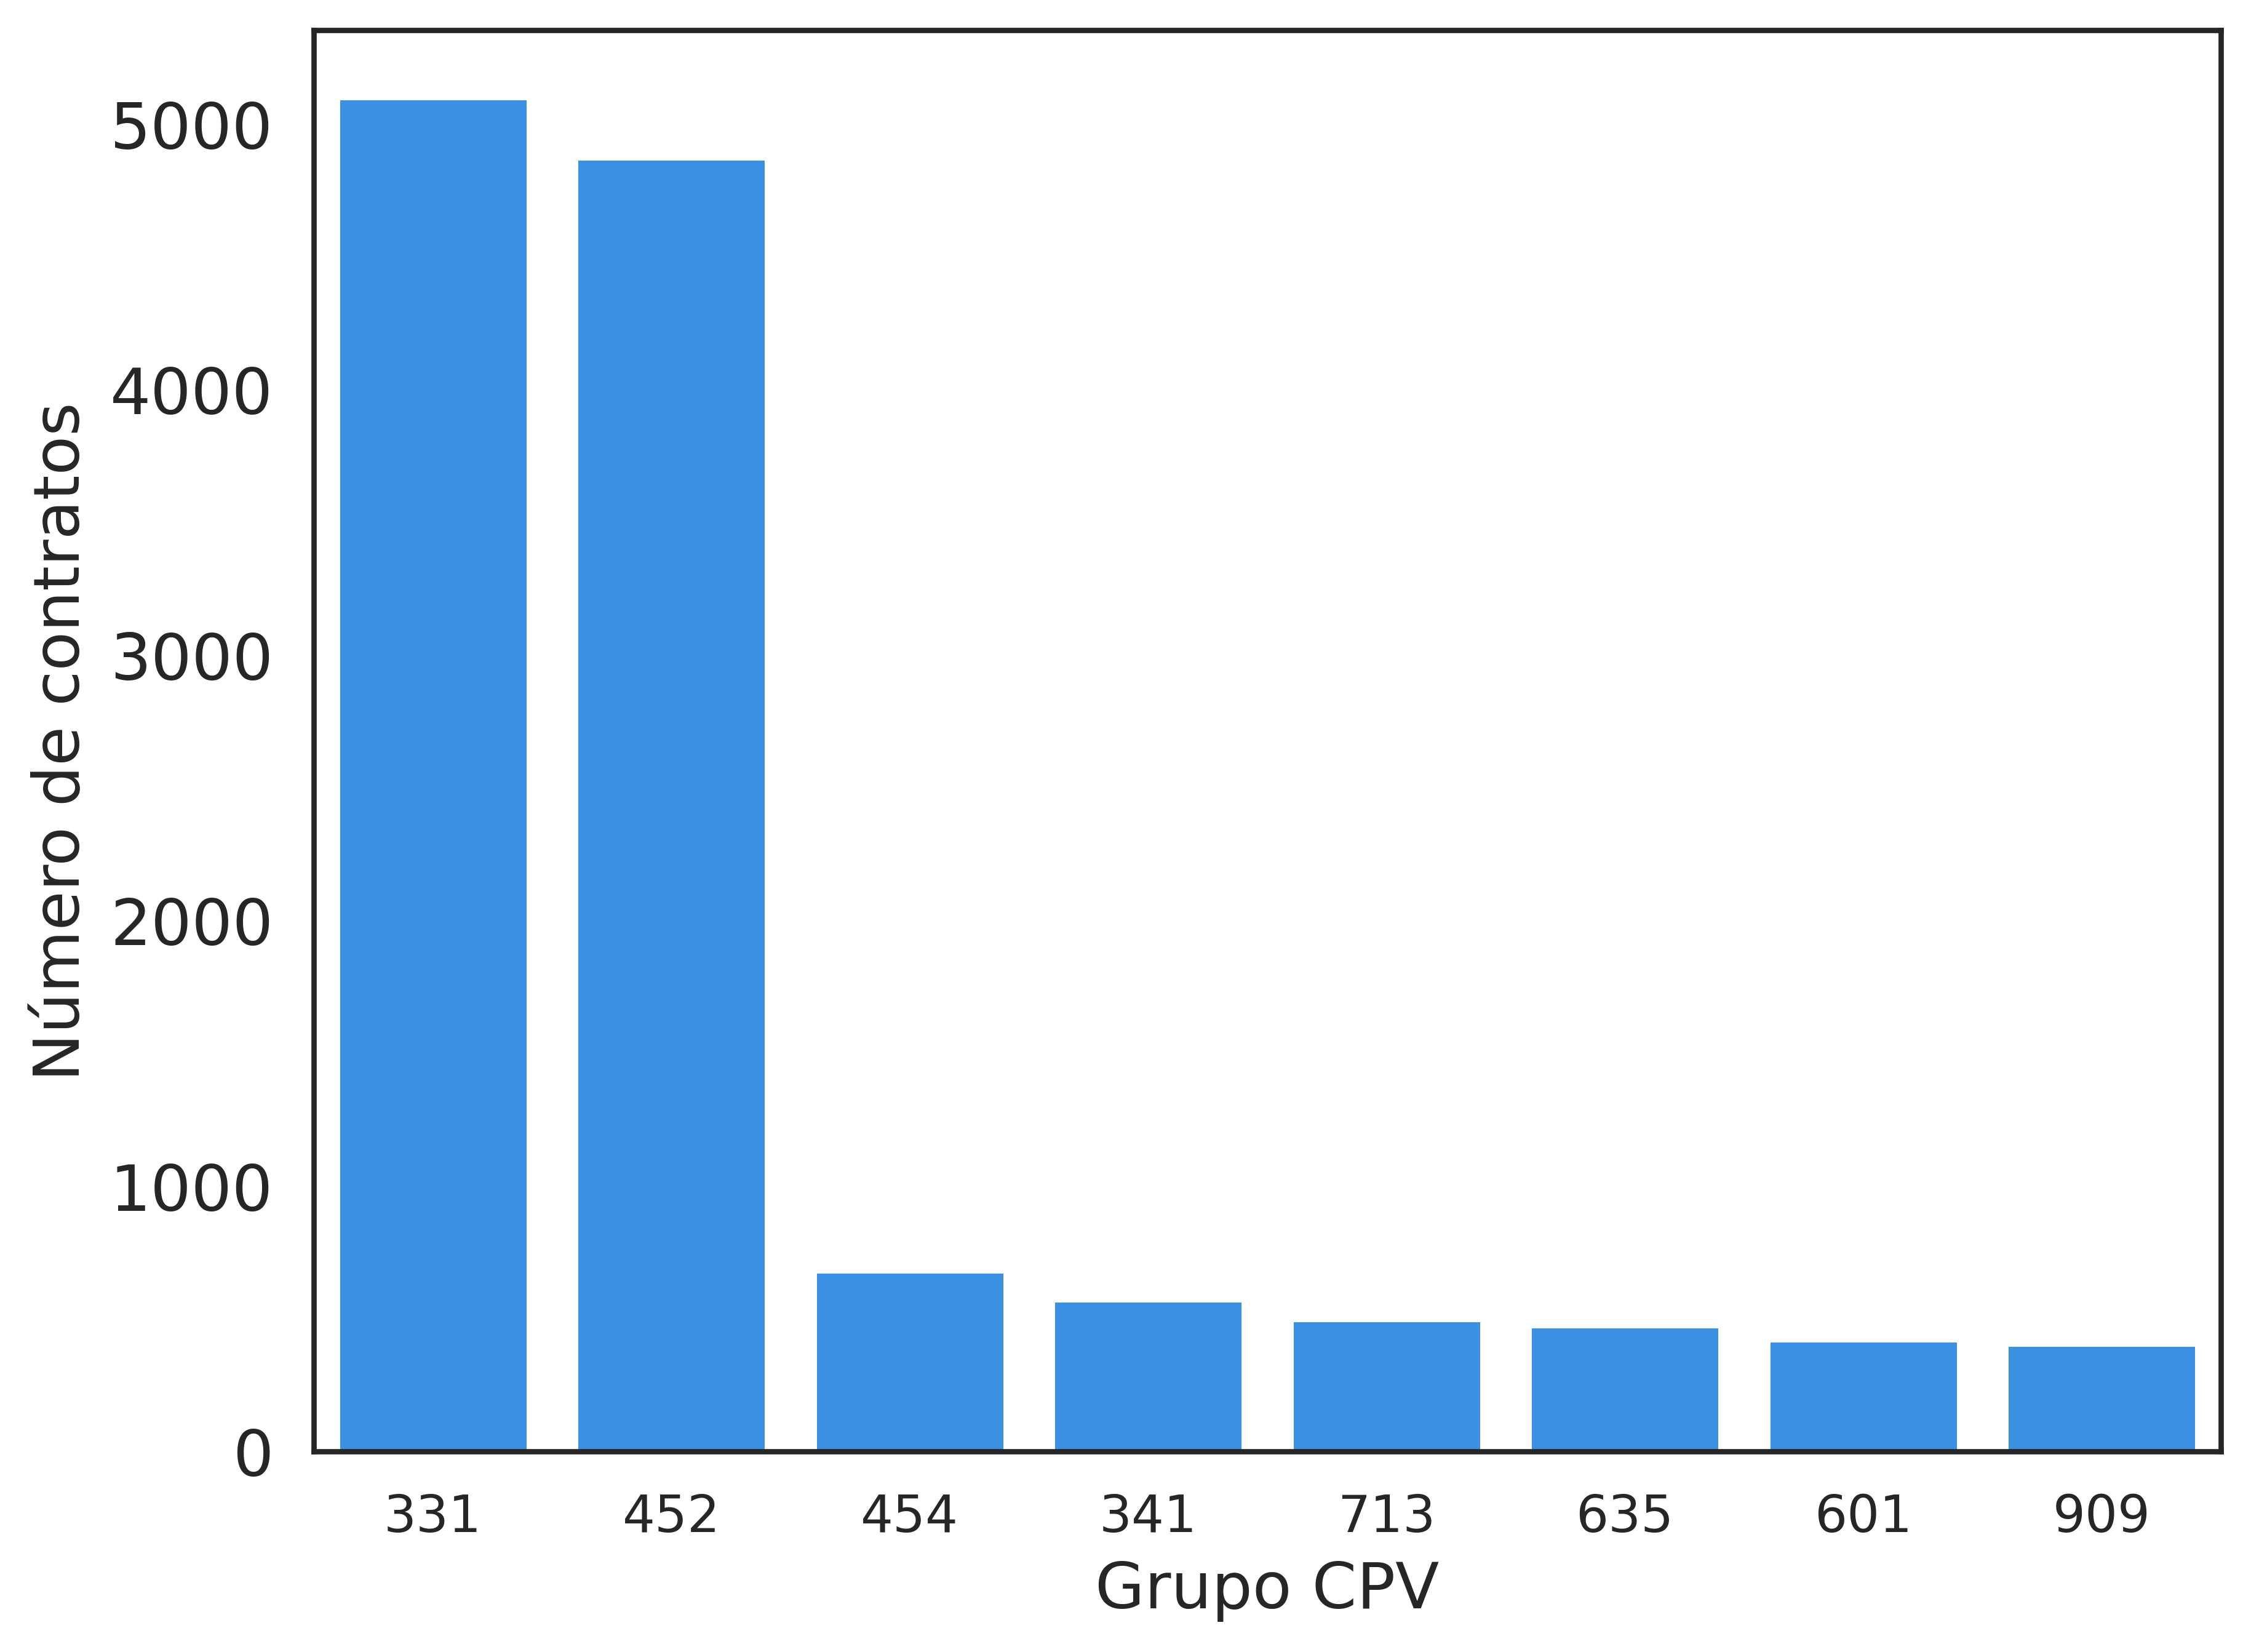
\includegraphics[width=\linewidth]{imagens/r017/cpvgroup.png}
		\caption{Grupos de CPV com maior número de contratos em inconformidade.}
	\end{minipage}
\end{figure}



Na Tabela \ref{tab:rf17stats} é possível confirmar o número de contratos sinalizados, para os principais grupos e divisões do CPV e respetivas percentagens do número total de contratos celebrados e sinalizados.

\begin{table}[H]
	\centering
	\renewcommand{\arraystretch}{1.15}
	\setlength{\tabcolsep}{15pt}
	\resizebox{\textwidth}{!} & \textbf{\begin{tabular}[c]{@{}c@{}}Número total \\ de contratos ($N_2$)\end{tabular}} & \textbf{$\frac{N_1}{N_{2}}$\%} \\ \hline
		45                   & 6128                                                                                        & 22.5                               & 22371                                                                                 & 27.4                           \\
		33                   & 5446                                                                                        & 19.9                               & 30419                                                                                 & 17.9                           \\ \hline
		\textbf{Grupo CPV} & \textbf{\begin{tabular}[c]{@{}c@{}}Número de contratos \\ sinalizados ($N_1$)\end{tabular}} & \textbf{$\frac{N_1}{N_{Total}}$\%} & \textbf{\begin{tabular}[c]{@{}c@{}}Número total de \\ contratos ($N_2$)\end{tabular}} & \textbf{$\frac{N_1}{N_{2}}$\%} \\ \hline
		331                  & 5098                                                                                        & 18.7                               & 20996                                                                                 & 24.3                           \\
		452                  & 4872                                                                                        & 17.8                               & 15635                                                                                 & 31.2                           \\
		454                  & 680                                                                                         & 2.5                                & 3611                                                                                  & 18.8                           \\
		341                  & 570                                                                                         & 2.1                                & 2781                                                                                  & 20.5                           \\ \hline
		331                  & \multicolumn{4}{l}{Equipamento Médico}                                                                                                                                                                                                                    \\
		452                  & \multicolumn{4}{l}{Obras de construção total ou parcial e obras de engenharia civil}                                                                                                                                                                      \\
		454                  & \multicolumn{4}{l}{Trabalho de conclusão de construção}                                                                                                                                                                                                   \\
		341                  & \multicolumn{4}{l}{Veículos motorizados}                                                                                                                                                                                                                  \\ \hline
	\end{tabular}%
	}
	\caption{Descrição do número de contratos, total e sinalizados, para os principais grupos e divisões de CPV. Definição das principais divisões do CPV.}
	\label{tab:rf17stats}
\end{table}


É possível observar na Figura \ref{fig:diffscpvs} como se encontram distribuídas as diferenças entre os preços contratuais e o valor máximo tolerado para cada grupo do CPV. No caso de contratos referentes ao grupo do CPV 452, \textbf{Obras de construção total ou parcial e obras de engenharia civil}, regista-se um desfasamento significativo entre os valores praticados e os valores \textit{tolerados}, dado que, pelo menos 50\% dos contratos ultrapassam em 500.000,00€ o valor máximo da extremidade superior.

\begin{figure}[H]
	\centering
	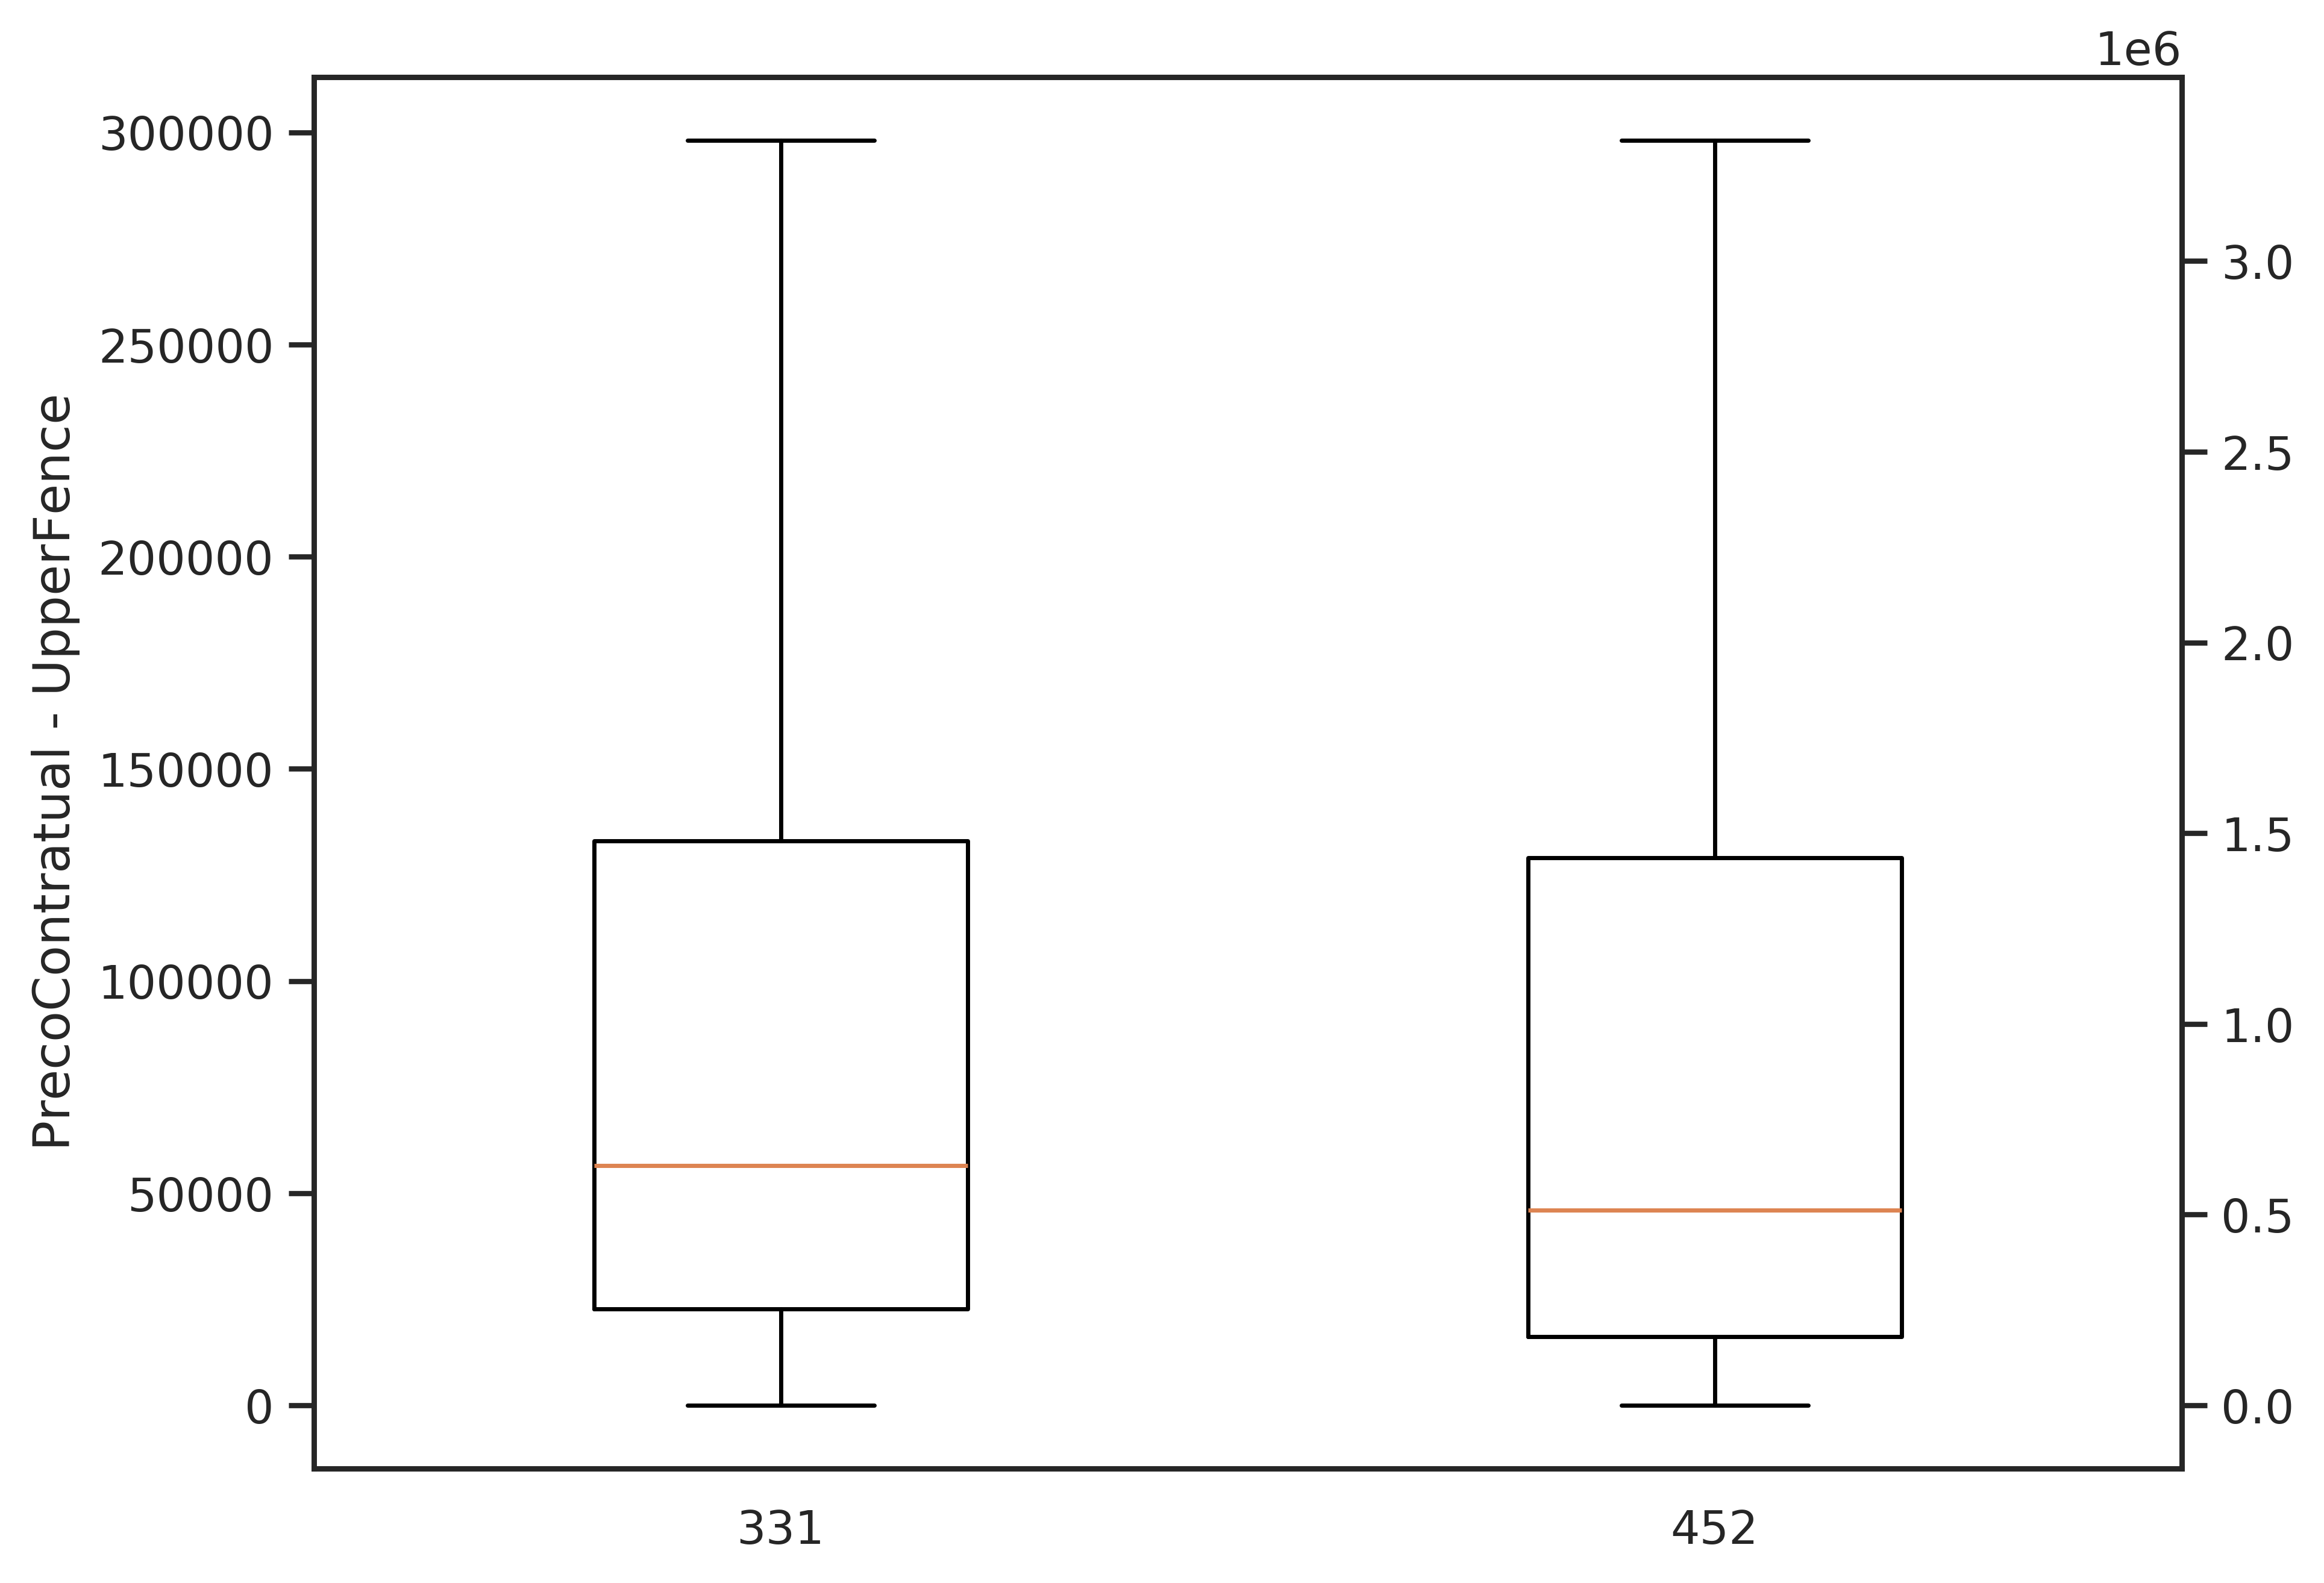
\includegraphics[width=0.6\textwidth]{imagens/r017/diffs.png}
	\caption{Boxplot da diferença dos preços contratuais e respetivas extremidades superiores para os grupos 331 e 452 do CPV.}
	\label{fig:diffscpvs}
\end{figure}




















\section{R018: Análise de concursos públicos com uma entidade concorrente}
\label{ch:entis}

Um dos parâmetros a respeitar aquando do estudo de um contrato público prende-se com a análise do número de entidades concorrentes. Partindo deste pressuposto, constatam-se três situações distintas ao longo do processo contratual: candidatura de apenas uma entidade, candidatura de um \textit{elevado} número de entidades e, por fim, candidatura de um \textit{reduzido} número de entidades. O indicador R018 proposto pela OCDS pretende, precisamente,  selecionar todos os contratos em que se verifique a participação de apenas um concorrente durante o processo de candidatura\footnote{Single bid received : Tender featured a single bidder only.}.

Atendendo a  que uma das colunas da tabela contempla a  identificação das entidades que se candidataram a um determinado concurso, é exequível uma análise ao número de entidades concorrentes. Na Tabela \ref{tab:entsconc} pode ser observado, de uma forma genérica, como é que esta coluna se encontra preenchida na base de dados. 


\begin{table}[H]
	\centering
	\begin{tabular}{|c|c|}
		\hline
		\textbf{ID}   & \textbf{EntidadesConcorrentes}                                                                                                      \\ \hline
		$\text{ID}_1$ & $\text{Entidade}\_i$ ( $\text{NIF}\_i$) $|||$ $\text{Entidade}\_j$ ( $\text{NIF}\_j$)                                               \\ \hline
		$\text{ID}_2$ & $\text{Entidade}\_k$ ( $\text{NIF}\_k$)                                                                                             \\ \hline
		$\dots$       & $\dots$                                                                                                                             \\ \hline
		$\text{ID}_n$ & $\text{Entidade}\_l$ ( $\text{NIF}\_l$) $|||$ $\text{Entidade}\_m$ ( $\text{NIF}\_m$) $|||$ $\text{Entidade}\_n$ ( $\text{NIF}\_n$) \\ \hline
	\end{tabular}
	\caption{Formato genérico da coluna \textbf{entidades\_concorrentes}.}
	\label{tab:entsconc}
\end{table}

Para cada entidade concorrente é inserido o respetivo nome e número de identificação fiscal (NIF). Quando o número de entidades concorrentes é superior a 1, a separação entre elas é feita recorrendo a um separador $|||$. Desta forma, foi necessário desenvolver uma \textit{query} que contabiliza o número de elementos separados e, posteriormente, insira o resultado numa nova coluna criada, chamada \textit{nr\_entidadesconcorrentes}.


\begin{lstlisting}[
	language=SQL,
	showspaces=false,
	basicstyle=\ttfamily,
	numbers=left,
	numberstyle=\tiny,
	commentstyle=\color{gray}, frame = single,
	breaklines=true,
	autogobble =true,
	postbreak=\mbox{\textcolor{red}{$\hookrightarrow$}\space},
	]
	UPDATE concursospublicos
	SET nr_entidadesconcorrentes = ARRAY_LENGTH(STRING_TO_ARRAY( entidades_concorrentes, '|||'), 1) + 1;	
\end{lstlisting}

Esta nova coluna possibilita a seleção imediata de todos os contratos que contemplem somente uma entidade concorrente.

\begin{lstlisting}[
	language=SQL,
	showspaces=false,
	basicstyle=\ttfamily,
	numbers=left,
	numberstyle=\tiny,
	commentstyle=\color{gray}, frame = single,
	breaklines=true,
	autogobble =true,
	postbreak=\mbox{\textcolor{red}{$\hookrightarrow$}\space},
	]
	SELECT contratos_basegov."id"
	FROM contratos_basegov
	JOIN concursos_publicos ON contratos_basegov."id" = concursos_publicos."id"
	WHERE concursos_publicos."nr_entidadesconcorrentes" = 1;
\end{lstlisting}


Da totalidade de concursos públicos celebrados, foram sinalizados cerca de 20\% ($N_{Total} =$ 25274) em que apenas se candidatou uma entidade. Na Tabela \ref{tab:rf18stats} representam-se as principais divisões do CPV relativas a contratos \textit{sinalizados} e respetivos valores.

\begin{table}[H]
	\centering
	\renewcommand{\arraystretch}{1.15}
	\setlength{\tabcolsep}{15pt}
	\resizebox{\textwidth}{!} & \textbf{\begin{tabular}[c]{@{}c@{}}Número total \\ de contratos ($N_2$)\end{tabular}} & \textbf{ $\frac{N_1}{N_{2}}$\%} & \textbf{\begin{tabular}[c]{@{}c@{}}Preço contratual\\ total\end{tabular}} \\ \hline
			33                   & 4444                                                                                & 27          & 29351                                                                         & 15.1        & 279.688.414,00€                                                           \\
			45                   & 3498                                                                                & 22          & 21525                                                                         & 16.3        & 2.103.391.451,00€                                                         \\
			15                   & 1625                                                                                & 10          & 5963                                                                          & 27.2        & 280.726.463,00€                                                           \\
			72                   & 1406                                                                                & 9           & 3739                                                                          & 37.6        & 65.760.473,00€                                                            \\
			34                   & 1162                                                                                & 7           & 4597                                                                          & 25.3        & 303.614.946,00€                                                           \\
			60                   & 1124                                                                                & 7           & 3512                                                                          & 32          & 351.923.997,00€                                                           \\
			50                   & 1069                                                                                & 6           & 3908                                                                          & 27.4        & 205.240.508,00€                                                           \\ \midrule
			\textbf{Total}       & 14328                                                                               & -           & 72595                                                                         & -           & -                                                                         \\ \hline
		\end{tabular}%
	}
	\caption{Descrição do número de contratos, total e sinalizados, para as principais divisões do CPV.}
	\label{tab:rf18stats}
\end{table}


\begin{figure}[H]
	\centering
	\begin{minipage}{.48\linewidth}
		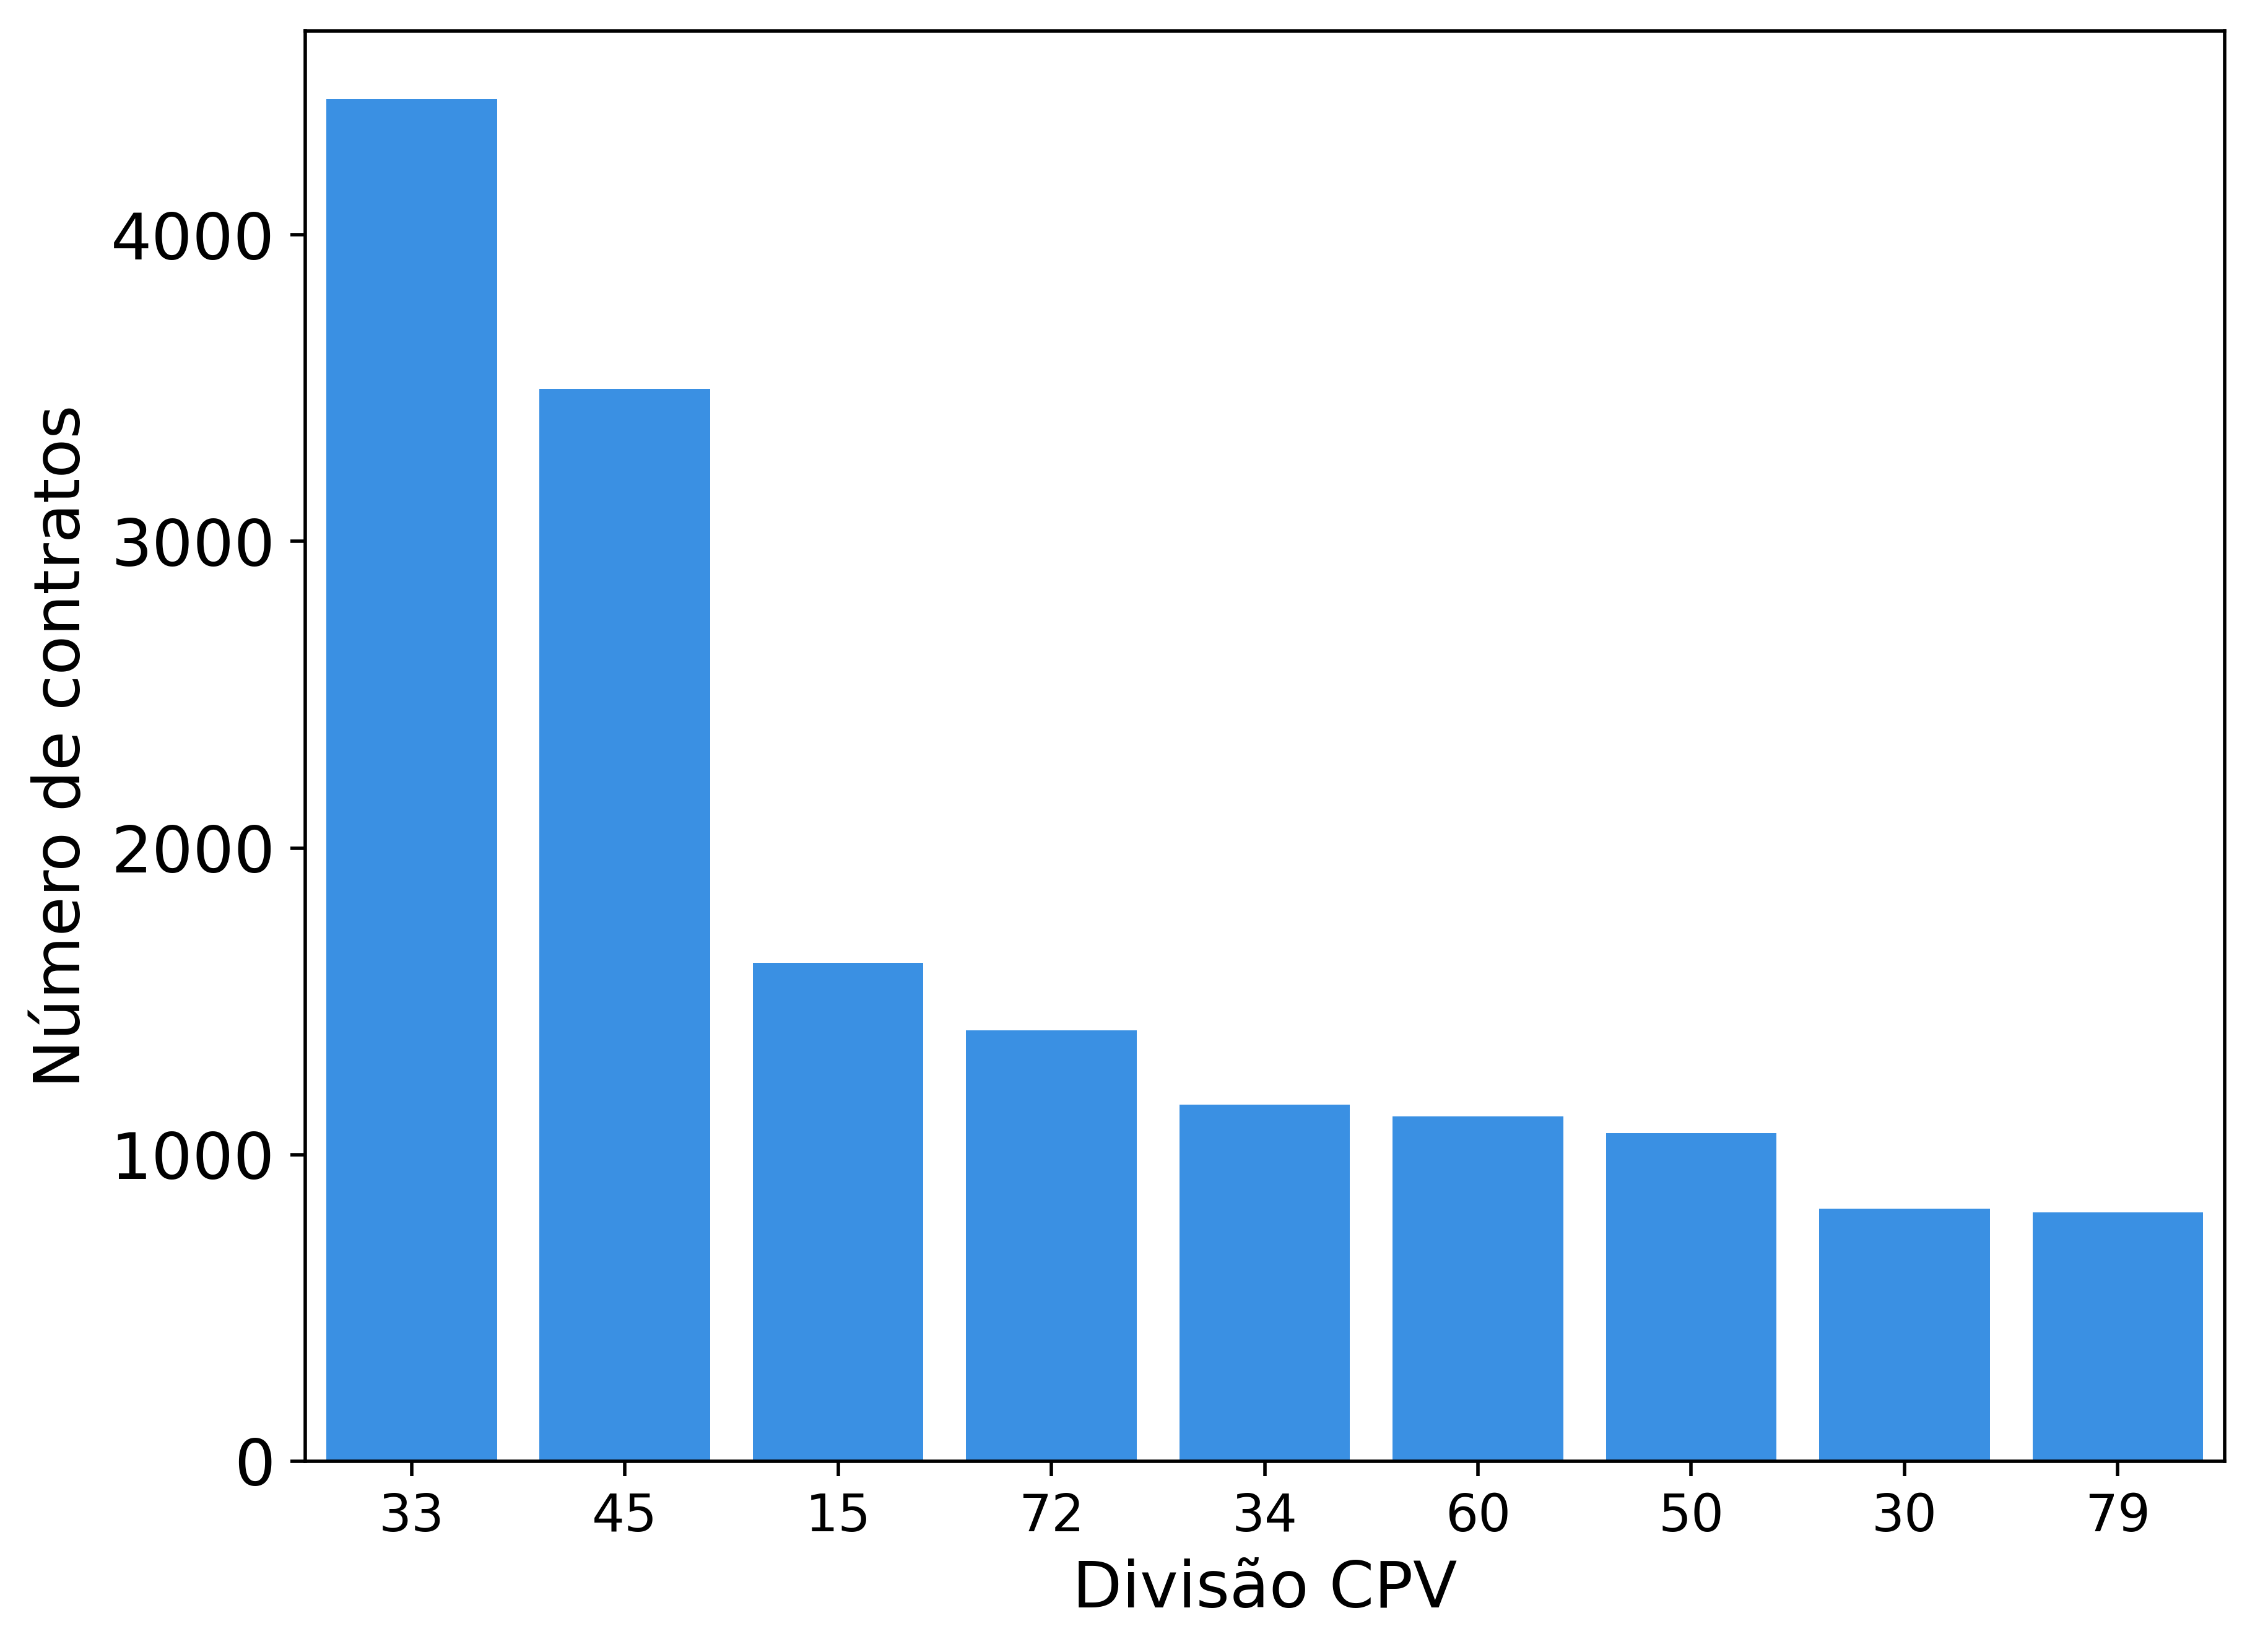
\includegraphics[width=\linewidth]{imagens/r018/main_cpvs.png}
		\caption{Divisões de CPV com maior número de contratos sinalizados.}
	\end{minipage}
	\hfill
	\begin{minipage}{.49\linewidth}
		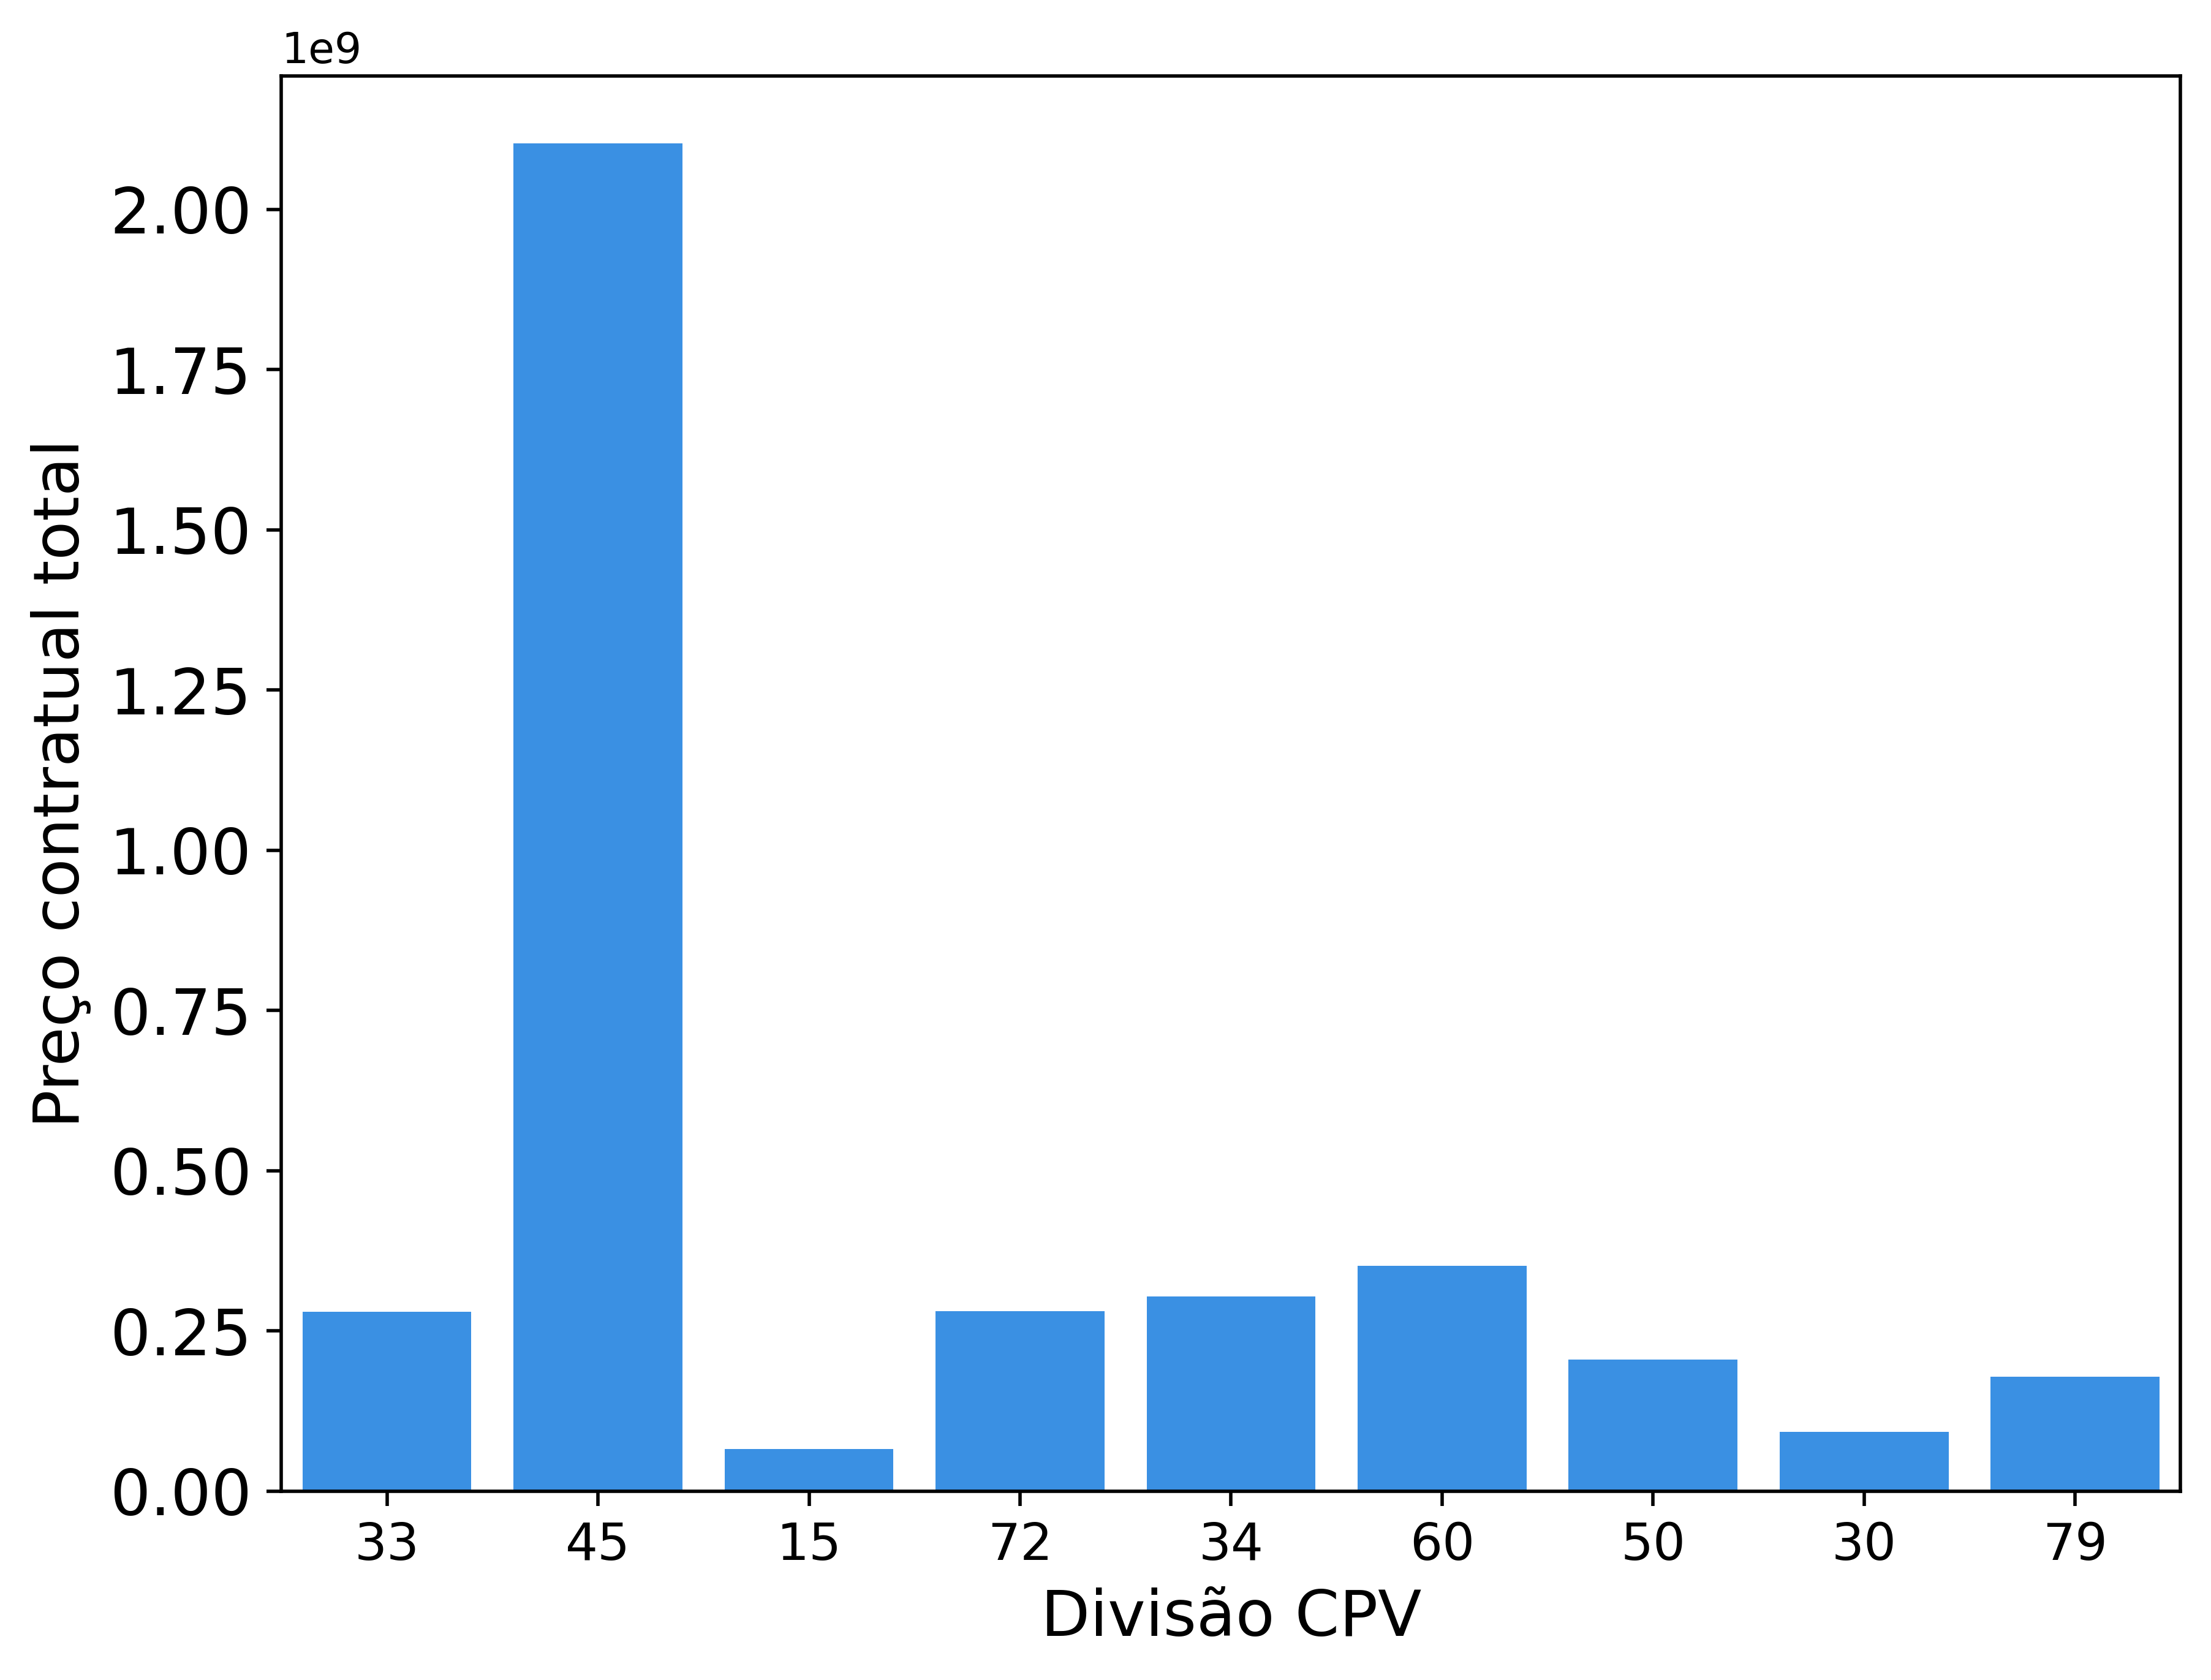
\includegraphics[width=\linewidth]{imagens/r018/prices.png}
		\caption{Valor adjudicado total para todos dos contratos sinalizados, por divisão do CPV.}
	\end{minipage}
\end{figure}










\section{R019: Análise do número de entidades concorrentes}

A aplicação deste indicador procura analisar se o número de entidades que concorrem a um determinado concurso público supera os limites inferior e superior expectáveis\footnote{Low number of bidders for item and procuring entity. Number of bidders significantly less than average, based on prior similar contracts (for similar item or procuring entity)}. Apesar de o indicador definido pela OCDS incidir apenas na análise de concursos públicos com um reduzido número de concorrentes, optou-se, ao desenvolver este indicador, por incluir uma barreira superior para detetar concursos com um elevado número de concorrentes. A inclusão deste passo foi motivada pela potencial presença de entidades concorrentes sem intenção de vencer e, desta forma, simularem um processo de livre concorrência.


Nas Figuras \ref{fig:distisnec} e \ref{fig:boxplotsnec} pode observar-se a distribuição do número de entidades concorrentes para cada divisão do CPV. Como se verifica, existe uma enorme variabilidade entre as diferentes divisões e, excetuando a divisão 41, todas as distribuições evidenciam uma nítida assimetria à direita.


Para a construção deste indicador foi utilizada a tabela auxiliar \textit{cpv\_stat}. A definição das barreiras inferior e superior para identificar os outliers, para cada divisão do CPV, obedeceu ao cálculo da constante de Medcouple para cada uma delas (divisão) e, consequentemente, definiram-se as respetivas extremidades. Assim, com o propósito de se selecionarem todos os contratos, cujo número de entidades concorrentes seja considerado um outlier, construíu-se a seguinte \textit{query}: 

\begin{lstlisting}[
	language=SQL,
	showspaces=false,
	basicstyle=\ttfamily,
	numbers=left,
	numberstyle=\tiny,
	commentstyle=\color{gray}, frame = single,
	breaklines=true,
	autogobble =true,
	postbreak=\mbox{\textcolor{red}{$\hookrightarrow$}\space},
	]
	SELECT contratos_basegov."id"
	FROM contratos_basegov 
	JOIN concursos_publicos ON contratos_basegov."id" = concursos_publicos."id"
	JOIN cpv_stat ON SUBSTRING(contratos_basegov."cpv", 1, 2) = cpv_stat."cpv"
	WHERE concursos_publicos."nr_entidadesconcorrentes" < lower_fence OR
		  concursos_publicos."nr_entidadesconcorrentes" > upper_fence;
	
\end{lstlisting}

Os resultados obtidos e que constam na Figura \ref{fig:necincump}, evidenciam uma forte predominância das divisões 33 e 45 do CPV. Da totalidade dos concursos públicos considerados, cerca de 18\% ($N_{Total} = 22951$)  foram sinalizados tendo em conta o presente indicador.


\begin{figure}[H]
	\centering
	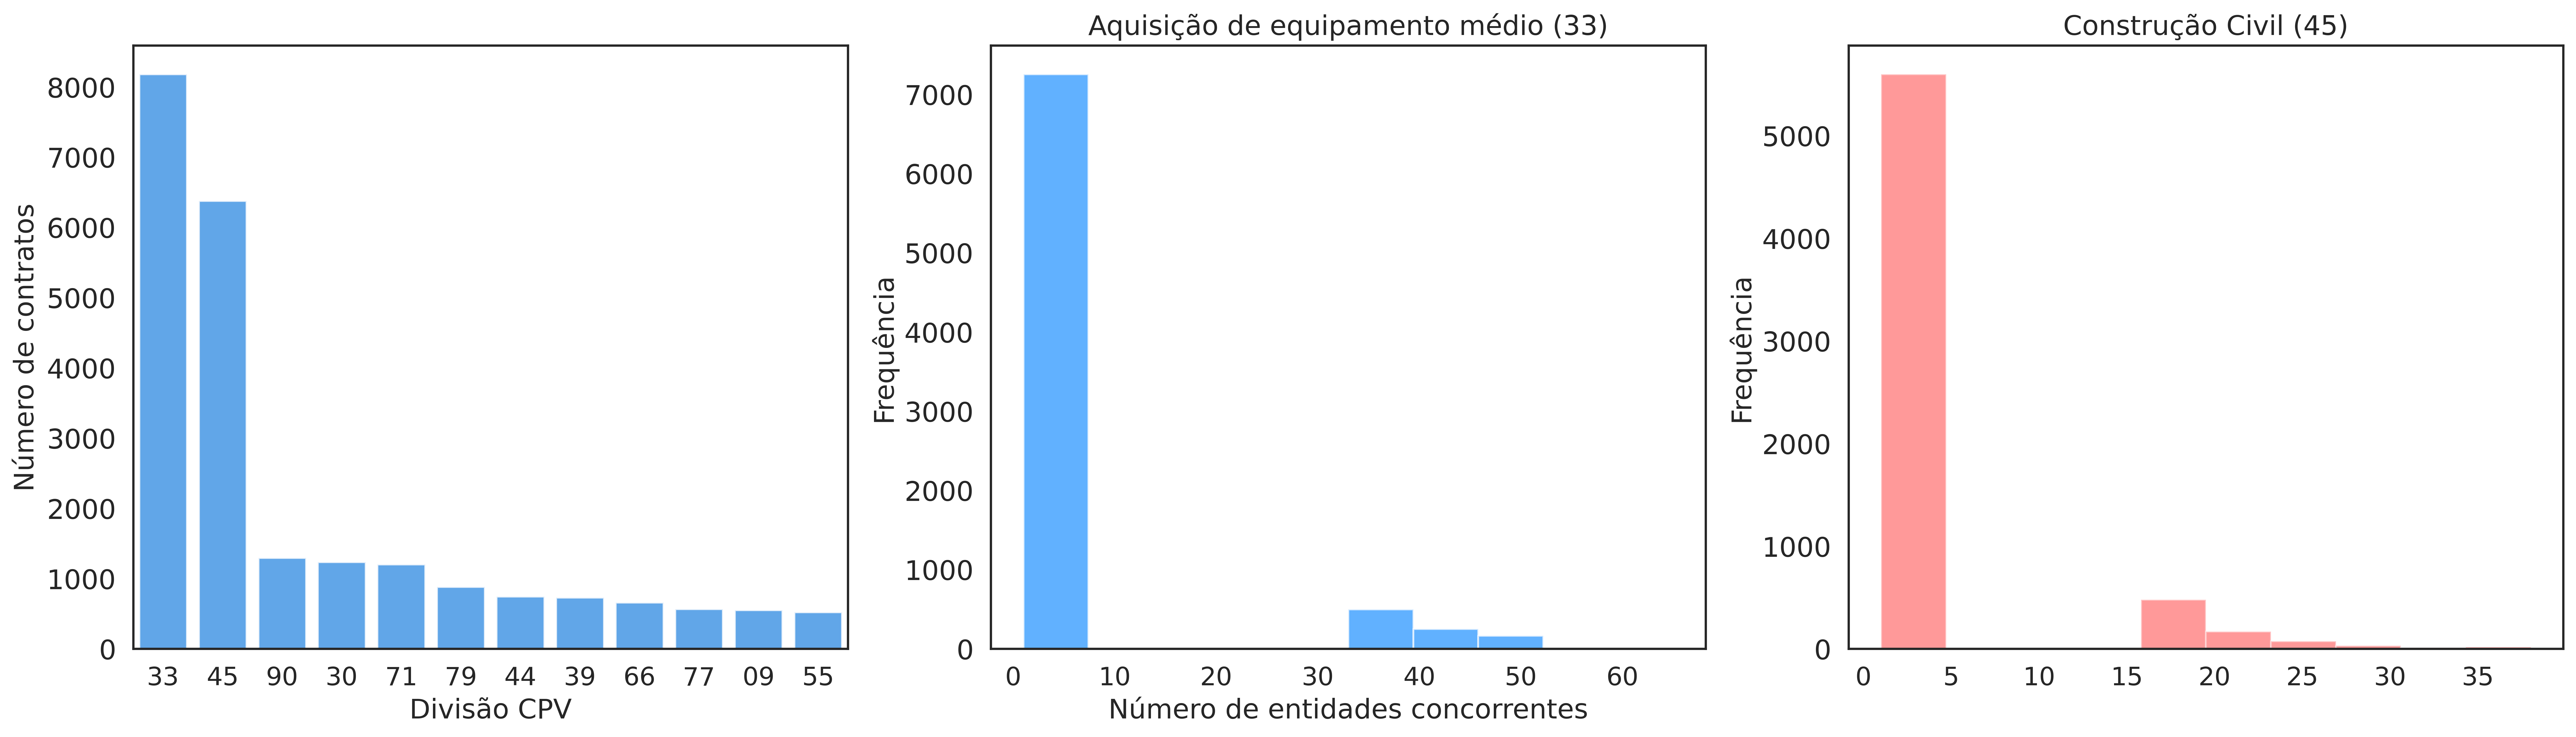
\includegraphics[width=\textwidth]{imagens/r019/colecao.png}
	\caption{Da esquerda para a direita: Divisões de CPV com maior número de contratos em inconformidade relativamente ao número de entidades concorrentes; Distribuição do número de outliers para as divisões 33 e 45, respetivamente.}
	\label{fig:necincump}
\end{figure}


\begin{table}[H]
	\centering
	\renewcommand{\arraystretch}{1.15}
	\setlength{\tabcolsep}{15pt}
	\resizebox{\textwidth}{!} & \textbf{\begin{tabular}[c]{@{}c@{}}\% Outliers\\ inferiores\end{tabular}} & \textbf{\begin{tabular}[c]{@{}c@{}}\% Outliers \\ superiores\end{tabular}} & \textbf{\begin{tabular}[c]{@{}c@{}}Número de \\ contratos total ($N_2$)\end{tabular}} & \textbf{$\frac{N_1}{N_{2}}$\%} & \textbf{\begin{tabular}[c]{@{}c@{}}Número máximo de\\ entidades concorrentes\end{tabular}} \\ \hline
		33                   & 8182                                                                                        & 35.6                               & 88.7                                                                      & 11.3                                                                       & 29351                                                                                 & 27.8                               & 65                                                                                        \\
		45                   & 6381                                                                                        & 27.8                               & 68.4                                                                      & 31.6                                                                       & 21525                                                                                 & 29.6                               & 38                                                                                        \\ \hline
	\end{tabular}%
	}
	\caption{Descrição do número de contratos, total e inconformes, para as principais divisões de CPV.}
	\label{tab:rf19stats}
\end{table}


Dos outliers detetados, considerando apenas as divisões 33 e 45 do CPV, constata-se que a maioria se posiciona abaixo da extremidade inferior, circunstância que remete para um elevado número de contratos celebrados com um número de entidades concorrentes reduzido. Relativamente à extremidade oposta da distribuição do número de entidades concorrentes, verificou-se que o número máximo de entidades concorrentes, num determinado concurso, para cada um destas divisões, foram 65 e 38, respetivamente.



\section{R031: Comparação entre preço base e preço contratual}

Um dos indicadores definidos pela OCDS incide na deteção de contratos cujo preço contratual seja muito próximo do preço base\footnote{Winning bid is within threshold value of budget or estimated price.}. No processo de construção deste indicador, a ocorrência de uma das seguintes situações foi constante, tendo todas sido consideradas na elaboração da \textit{query} final:

\begin{my_enumerate}
	
	\item O valor do preço base para um determinado contrato ou era 0 ou não se encontrava preenchido (\textit{None}). \label{ponto1}
	
	\item O valor do preço contratual era superior ao valor do preço base. \label{ponto2}
	
	\item O valor do preço contratual era inferior ao valor do preço base.
	
\end{my_enumerate}

Como foi constatado anteriormente, nos termos do CCP, o preço base é definido como o montante máximo que a entidade adjudicante se dispõe a pagar pela execução do objeto contratual \cite{precobase}. Procedeu-se à adaptação deste indicador de forma a incluir o mecanismo de deteção de todos os contratos em que o preço contratual é superior ao preço base, criando-se, assim, a zona de \textit{rejeição II}.

%Desta forma, este indicador foi adaptado de forma a incluir o mecanismo de deteção de todos os contratos em que o preço contratual é superior ao preço base, criando-se, assim, a \textit{zona de rejeição II}. 

É de ressalvar que na elaboração deste indicador não foram considerados contratos ao abrigo do regime especial de adjudicação por lotes. O motivo pela qual se optou pela referida exclusão, prende-se com o facto de, contratualmente, cada lote ter um preço base associado e, no Portal BASE, o preço base ser definido, de igual forma, para todos os lotes. Na Tabela \ref{tab:lotes} encontra-se um exemplo de um contrato adjudicado por lotes. Na última coluna, \textbf{Preço Base Real}, encontram-se os preços base para cada lote. É de sublinhar, contudo, que estes valores foram obtidos a partir do documento PDF, onde é finalizado o contrato, e que se encontra disponível, apenas em alguns contratos, para consulta no Portal BASE. Em virtude de não se afigurar viável a criação de um mecanismo de obtenção dos preços base por cada lote existente, optou-se pela sua exclusão.


\begin{table}[H]
	\centering
	\renewcommand{\arraystretch}{1.15}
	\setlength{\tabcolsep}{15pt}
	\resizebox{\textwidth}{!}{%
	\begin{tabular}{ccccc
			>{\columncolor[HTML]{ECECEC}}c }
		\hline
		\textbf{Número de Anúncio}   & \textbf{ID} & \textbf{Lote} & \textbf{Preço Base}           & \textbf{Preço Contratual} & \textit{\textbf{Preço Base Real}} \\ \hline
		& 10471090    & 1             &                               & 77.454,72€                & \textit{129.276,00€}              \\
		& 10471049    & 2             &                               & 85.365,84€                & \textit{104.072,64€}              \\
		& 10470972    & 3             &                               & 89.886,72€                & \textit{104.072,64€}              \\
		\multirow{-4}{*}{11171/2023} & 10539451    & 4             & \multirow{-4}{*}{373.860,48€} & 29.075,76€                & \textit{36.439,20€}               \\ \hline
	\end{tabular}%
	}
	\caption{Exemplo de um contrato adjudicado por lotes.}
\label{tab:lotes}
\end{table}






Assim, com o objetivo de incluir os primeiros dois pontos mencionados em \ref{ponto1} e \ref{ponto2} e detetar todos os contratos com um preço contratual \textit{próximo} do preço base, construiu-se a seguinte \hyperref[lst:r31]{função}, definida em \ref{lst:r31}. Esta função tem como parâmetro de entrada um valor máximo de tolerância $\epsilon$ cuja finalidade é definir a \textit{zona de rejeição I}. Estas zonas de rejeição encontram-se ilustradas na Figura \ref{fig:rej}.

\begin{figure}[H]
	\centering
	
\includegraphics[width=.8\textwidth]{imagens/r31/r31.png}
	\caption{Ilustração das zonas de rejeição do preço contratual. }
	\label{fig:rej}
\end{figure}

Em suma, a deteção de contratos que obedecem às condições impostas por este indicador seguem o processo ilustrado na Figura \ref{fig:r31}. 

\begin{figure}[H]
	\centering
	
\includegraphics[width=\textwidth]{imagens/r31/r31procss.png}
	\caption{Ilustração do processo de deteção de contratos sinalizados. }
	\label{fig:r31}
\end{figure}

Verificou-se que na base de dados, 20 dos concursos públicos continham preço base nulo e 3597 não continham este campo preenchido. Consequentemente, estes foram descartados do processo de comparação. 
Dentro da primeira e segunda zona de rejeição, apuraram-se 35967 e 348 contratos celebrados, respetivamente. Para efeitos de demonstração, o nível de tolerância utilizado nesta análise foi de $0.1$. Assim sendo, são sinalizados todos os contratos cujo preço contratual seja superior a $90\%$ do preço base. Esta abordagem não se revelou como a mais eficiente, já que diferentes níveis de tolerância devem ser considerados consoante a categoria do contrato, atendendo à agregação por grupo ou divisão do CPV. O resultado final encontra-se ilustrado na Tabela \ref{tab:r31vales}. 

\begin{table}[H]
	\centering
	\renewcommand{\arraystretch}{1.15}
	\setlength{\tabcolsep}{15pt}
	\resizebox{\textwidth}{!}{%
	\begin{tabular}{clcl|cc|cc}
		\hline
		\multicolumn{4}{c|}{\textbf{Preço Base}}                                        & \multicolumn{2}{c|}{\multirow{2}{*}{\textbf{Zona de rejeição I}}} & \multicolumn{2}{c}{\multirow{2}{*}{\textbf{Zona de rejeição II}}} \\
		\multicolumn{2}{c}{\textbf{Nulo}}          & \multicolumn{2}{c|}{\textbf{None}} & \multicolumn{2}{c|}{}                                             & \multicolumn{2}{c}{}                                              \\ \hline
		3497 & \multicolumn{1}{l|}{\textit{2.7\%}} & 20        & \textit{0.02\%}        & 35967                      & \textit{27.6\%}                      & 348                       & \textit{0.26\%}                       \\ \hline
	\end{tabular}%
	}
	\caption{Número de contratos sinalizados e respetivas percentagens.}
	\label{tab:r31vales}
\end{table}

Nas Figuras \ref{fig:r31nulos}, \ref{fig:r31nulos2} e \ref{fig:r31nulo3} podem observar-se as distribuições do número de concursos públicos cujo valor do preço base no Portal BASE é nulo, cujo valor do preço contratual é superior ao preço base e cujo valor valor do preço contratual é muito próximo do preço base, por divisão do CPV.

Antes da celebração de um contrato, o preço base é conhecido e, desta forma, esta flag não acrescente informação relevante, se considerada de forma isolada. Quando acoplada a outras flags pode sugerir um comportamento questionável. 

Por outro lado, é preciso ter em conta o cálculo do preço base e se o mesmo se posiciona dentro do preço de mercado. Se o preço base for calculado por excesso e o preço contratual for próximo do preço base, poderão existir indícios de uma situação anómala.





\section{R051: Análise da concentração de mercado}


Com a construção deste indicador procurou-se averiguar a existência de empresas com uma eleavada concentração de concursos adjudicados, para determinado mercado\footnote{A small number of companies concentrate a high share of contracts in a particular market.}. 
As diretrizes da OCDS sugerem que se calcule a proporção de contratos ganhos por uma determinada entidade adjudicatária e a proporção do valor total adjudicado, para um determinado período de tempo (por exemplo, um ano). Na elaboração deste indicador optou-se por duas abordagens, tendo sido aplicadas, apenas, a contratos alusivos à comercialização de energia e gás.


%Este indicador foi desenvolvido e aplicado apenas para contratos de comercialização de energia, água e gás. 



\subsection{Abordagem 1}

Com esta abordagem pretendeu-se avaliar a existência  de uma eventual tendência de um grupo restrito de empresas vencerem a maioria dos concursos públicos, para um determinado grupo do CPV. O processo encontra-se ilustrado na Figura \ref{fig:ab1}. 

\begin{figure}[H]
	\centering
	
\includegraphics[width=0.9\textwidth]{imagens/r51/r51_v2.png}
	\caption{Ilustração do processo da abordagem 1.}
\label{fig:ab1}
\end{figure}

Sempre que um contrato é analisado, procede-se à identificação do grupo do CPV. Seguidamente, determina-se o número total de contratos celebrados para esse mesmo grupo de CPV, ao longo de um determinado período de tempo\footnote{Ao longo do desenvolvimento deste indicador, o período de tempo considerado consistiu nos 12 meses precedentes à data de celebração do contrato.}, guardando-se o resultado na variável $X_1$. Após este passo, identifica-se a entidade adjudicatária do concurso em análise e calcula-se o número de contratos ganhos para o mesmo grupo do CPV, ao longo do mesmo período de tempo, guardando-se o resultado na variável $X_2$. Por fim, é calculado o rácio entre $X_2$ e $X_1$, com o objetivo de calcular a proporção de concursos ganhos por determinada entidade, num determinado mercado. 

De seguida, é determinado o valor adjudicado para a totalidade de concursos atribuídos à entidade adjudicatária, para a mesma divisão do CPV e período de tempo, guardando-se o resultado em $Y_1$. Por fim, é calculado o valor adjudicado para a totalidade de contratos celebrados referentes à categoria de CPV, no mesmo período de tempo considerado e guarda-se o resultado em $Y_2$.  Procede-se ao cálculo do rácio entre $Y_1$ e $Y_2$ com o objetivo de calcular a proporção do valor total adjudicado, dentro de um determinado mercado, para uma só entidade. 

Na Tabela \ref{tab:r51exemplo1} encontra-se um exemplo meramente ilustrativo da aplicação desta abordagem, cujos valores foram gerados aleatoriamente. Finda a seleção de todos os contratos de um grupo do CPV, registam-se 1564 contratos adjudicados num valor total de 4.020.343,00€. Da totalidade de contratos celebrados, a Empresa A venceu 257 concursos, adjudicados num total de 792.640,00€, a Empresa B venceu 1271, adjudicados num total de 3.144.952,00€ e a Empresa C venceu 38, ajudicados num valor total de 92.751,00€. Ao calcular os respetivos rácios, percebe-se que a Empresa B superou as concorrentes ao celebrar um maior número de contratos, bem como na respetiva fração do valor adjudicado, face ao valor total alocada à divisão do CPV. Tal facto pode ser revelador de uma situação tendenciosa.


\begin{table}[H]
	\centering
	\renewcommand{\arraystretch}{1.15}
	\setlength{\tabcolsep}{15pt}
	\resizebox{\textwidth}{!}{%
	\begin{tabular}{ccccccc}
		\cline{2-7}
		& \textbf{\begin{tabular}[c]{@{}c@{}}Número de contratos \\ celebrados, por empresa, \\ para grupo de CPV\end{tabular}} & \textbf{\begin{tabular}[c]{@{}c@{}}Número total de  \\ contratos celebrados,\\  para grupo de CPV\end{tabular}} & \textbf{Rácio} & \textbf{\begin{tabular}[c]{@{}c@{}}Valor total adjudicado \\ por empresa para\\  grupo de CPV\end{tabular}} & \textbf{\begin{tabular}[c]{@{}c@{}}Valor total \\ adjudicado por \\ grupo de CPV\end{tabular}} & \textbf{Rácio} \\ \hline
		\textbf{Empresa A} & 257                                                                                                                   & \multirow{3}{*}{1564}                                                                                          & 0.16           & 792.640,00€                                                                                                 & \multirow{3}{*}{4.020.343,00€}                                                                 & 0.19           \\
		\textbf{Empresa B} & 1271                                                                                                                  &                                                                                                                & 0.81           & 3.144.952,00€                                                                                               &                                                                                                & 0.78           \\
		\textbf{Empresa C} & 38                                                                                                                    &                                                                                                                & 0.03           & 92.751,00€                                                                                                  &                                                                                                & 0.023          \\ \hline
	\end{tabular}%
	}
	\caption{Exemplo da abordagem 1 para um conjunto de empresas fictícias, de um determinado grupo do CPV.}
	\label{tab:r51exemplo1}
\end{table}



\subsection{Abordagem 2}

Esta abordagem teve como objetivo verificar se existia uma tendência de determinadas entidades adjudicantes celebrarem concursos públicos sempre com empresas pertencentes a um grupo restrito. O processo desenvolvido apresenta-se ilustrado na Figura \ref{fig:ab2}. 

\begin{figure}[H]
	\centering
	
\includegraphics[width=0.9\textwidth]{imagens/r51/r51_v1.png}
	\caption{Ilustração do processo da abordagem 2.}
	\label{fig:ab2}
\end{figure}

O processo inicia-se com a identificação do grupo do CPV do contrato a analisar. Num segundo momento, é identificada a entidade adjudicante através do respetivo NIF, representado por $\text{NIF}_1$, e calcula-se o número de contratos celebrados por esta mesma entidade, ao longo de um período de tempo, para o grupo de CPV em questão, guardando-se o resultado na variável $X_1$. De seguida, é identificada a entidade adjudicatária através do respetivo NIF, representado por $\text{NIF}_2$, e é calculado o número de contratos celebrados entre $\text{NIF}_1$ e $\text{NIF}_2$, para o mesmo grupo de CPV e no mesmo período de tempo, guardando-se o resultado em $X_2$. Por fim, é calculado o rácio entre $X_1$ e $X_2$. Os valores do rácio variam entre zero e um, sendo que, valores muito próximos da unidade podem indiciar uma predisposição de contratação de serviços apenas de uma determinada empresa. 

Na Tabela \ref{tab:r51exemplo} exemplifica-se a aplicação da abordagem 2. Para um determinado contrato, deteta-se que uma entidade adjudicante celebrou 300 contratos, para uma determinada categoria de CPV, ao longo dos últimos 12 meses. Estes contratos foram celebrados apenas com três empresas, sendo 193 deles com a Empresa A, 12 com a Empresa B e 95 com a Empresa C. Na sequência do cálculo dos rácios, constata-se que este valor, para os contratos celebrados entre a entidade adjudicante e a Empresa A, se destaca dos demais, podendo ser revelador de um comportamento duvidoso. 

\begin{table}[H]
	\centering
	\renewcommand{\arraystretch}{1.15}
	\setlength{\tabcolsep}{15pt}
	\resizebox{\textwidth}{!}{%
		\begin{tabular}{c|cc|c}
			\hline
			\textbf{\begin{tabular}[c]{@{}c@{}}Entidade\\ Adjudicante\end{tabular}} &                    & \textbf{\begin{tabular}[c]{@{}c@{}}Número de contratos\\ celebrados para grupo de CPV\end{tabular}} & \textbf{Rácio} \\ \hline
			\multirow{3}{*}{300}                                                    & \textbf{Empresa A} & 193                                                                                                 & 0.64           \\
			& \textbf{Empresa B} & 12                                                                                                  & 0.04           \\
			& \textbf{Empresa C} & 95                                                                                                  & 0.32           \\ \hline
		\end{tabular}%
	}
	\caption{Exemplo de ilustração da abordagem 2 para uma entidade adjudicante e conjunto de empresas fictícias.}
	\label{tab:r51exemplo}
\end{table}



\section{RF2: Comparação entre preço contratual e preço total efetivo}

Existem situações em que o valor contratual celebrado é alterado após a celebração do contrato, seja por se entender não existir necessidade de aplicar todos os recursos previstos, ou pelo seu contrário. Contudo, tal como foi visto anteriormente, também existem casos em que este campo diz respeito ao preço contratual referente à prestação completa de um serviço e o preço contratual diz respeito ao preço acordado por unidade (por exemplo: metro quadrado, quilómetro, hora, dia). Estes valores são guardados na coluna referefente ao Preço Total Efetivo. Nesses casos, é simples verificar quais são os contratos em que ocorre esta situação através de uma \textit{query}: 


%\begin{lstlisting}[
%	language=SQL,
%	showspaces=false,
%	basicstyle=\ttfamily,
%	numbers=left,
%	numberstyle=\tiny,
%	commentstyle=\color{gray},	frame=single,
%	breaklines=true,
%	autogobble = true,
%	postbreak=\mbox{\textcolor{red}{$\hookrightarrow$}\space},
%	]
%	SELECT contratos_basegov."id", 
%	FROM contratos_basegov 
%	WHERE contratos_basegov."totalEffectivePrice" > 0 AND 
%		ABS(contratos_basegov."totalEffectivePrice" - preco_contratual) > 0 AND 
%		preco_contratual > 0;
%\end{lstlisting}
%
%
%\begin{figure}[H]
%	\centering
%	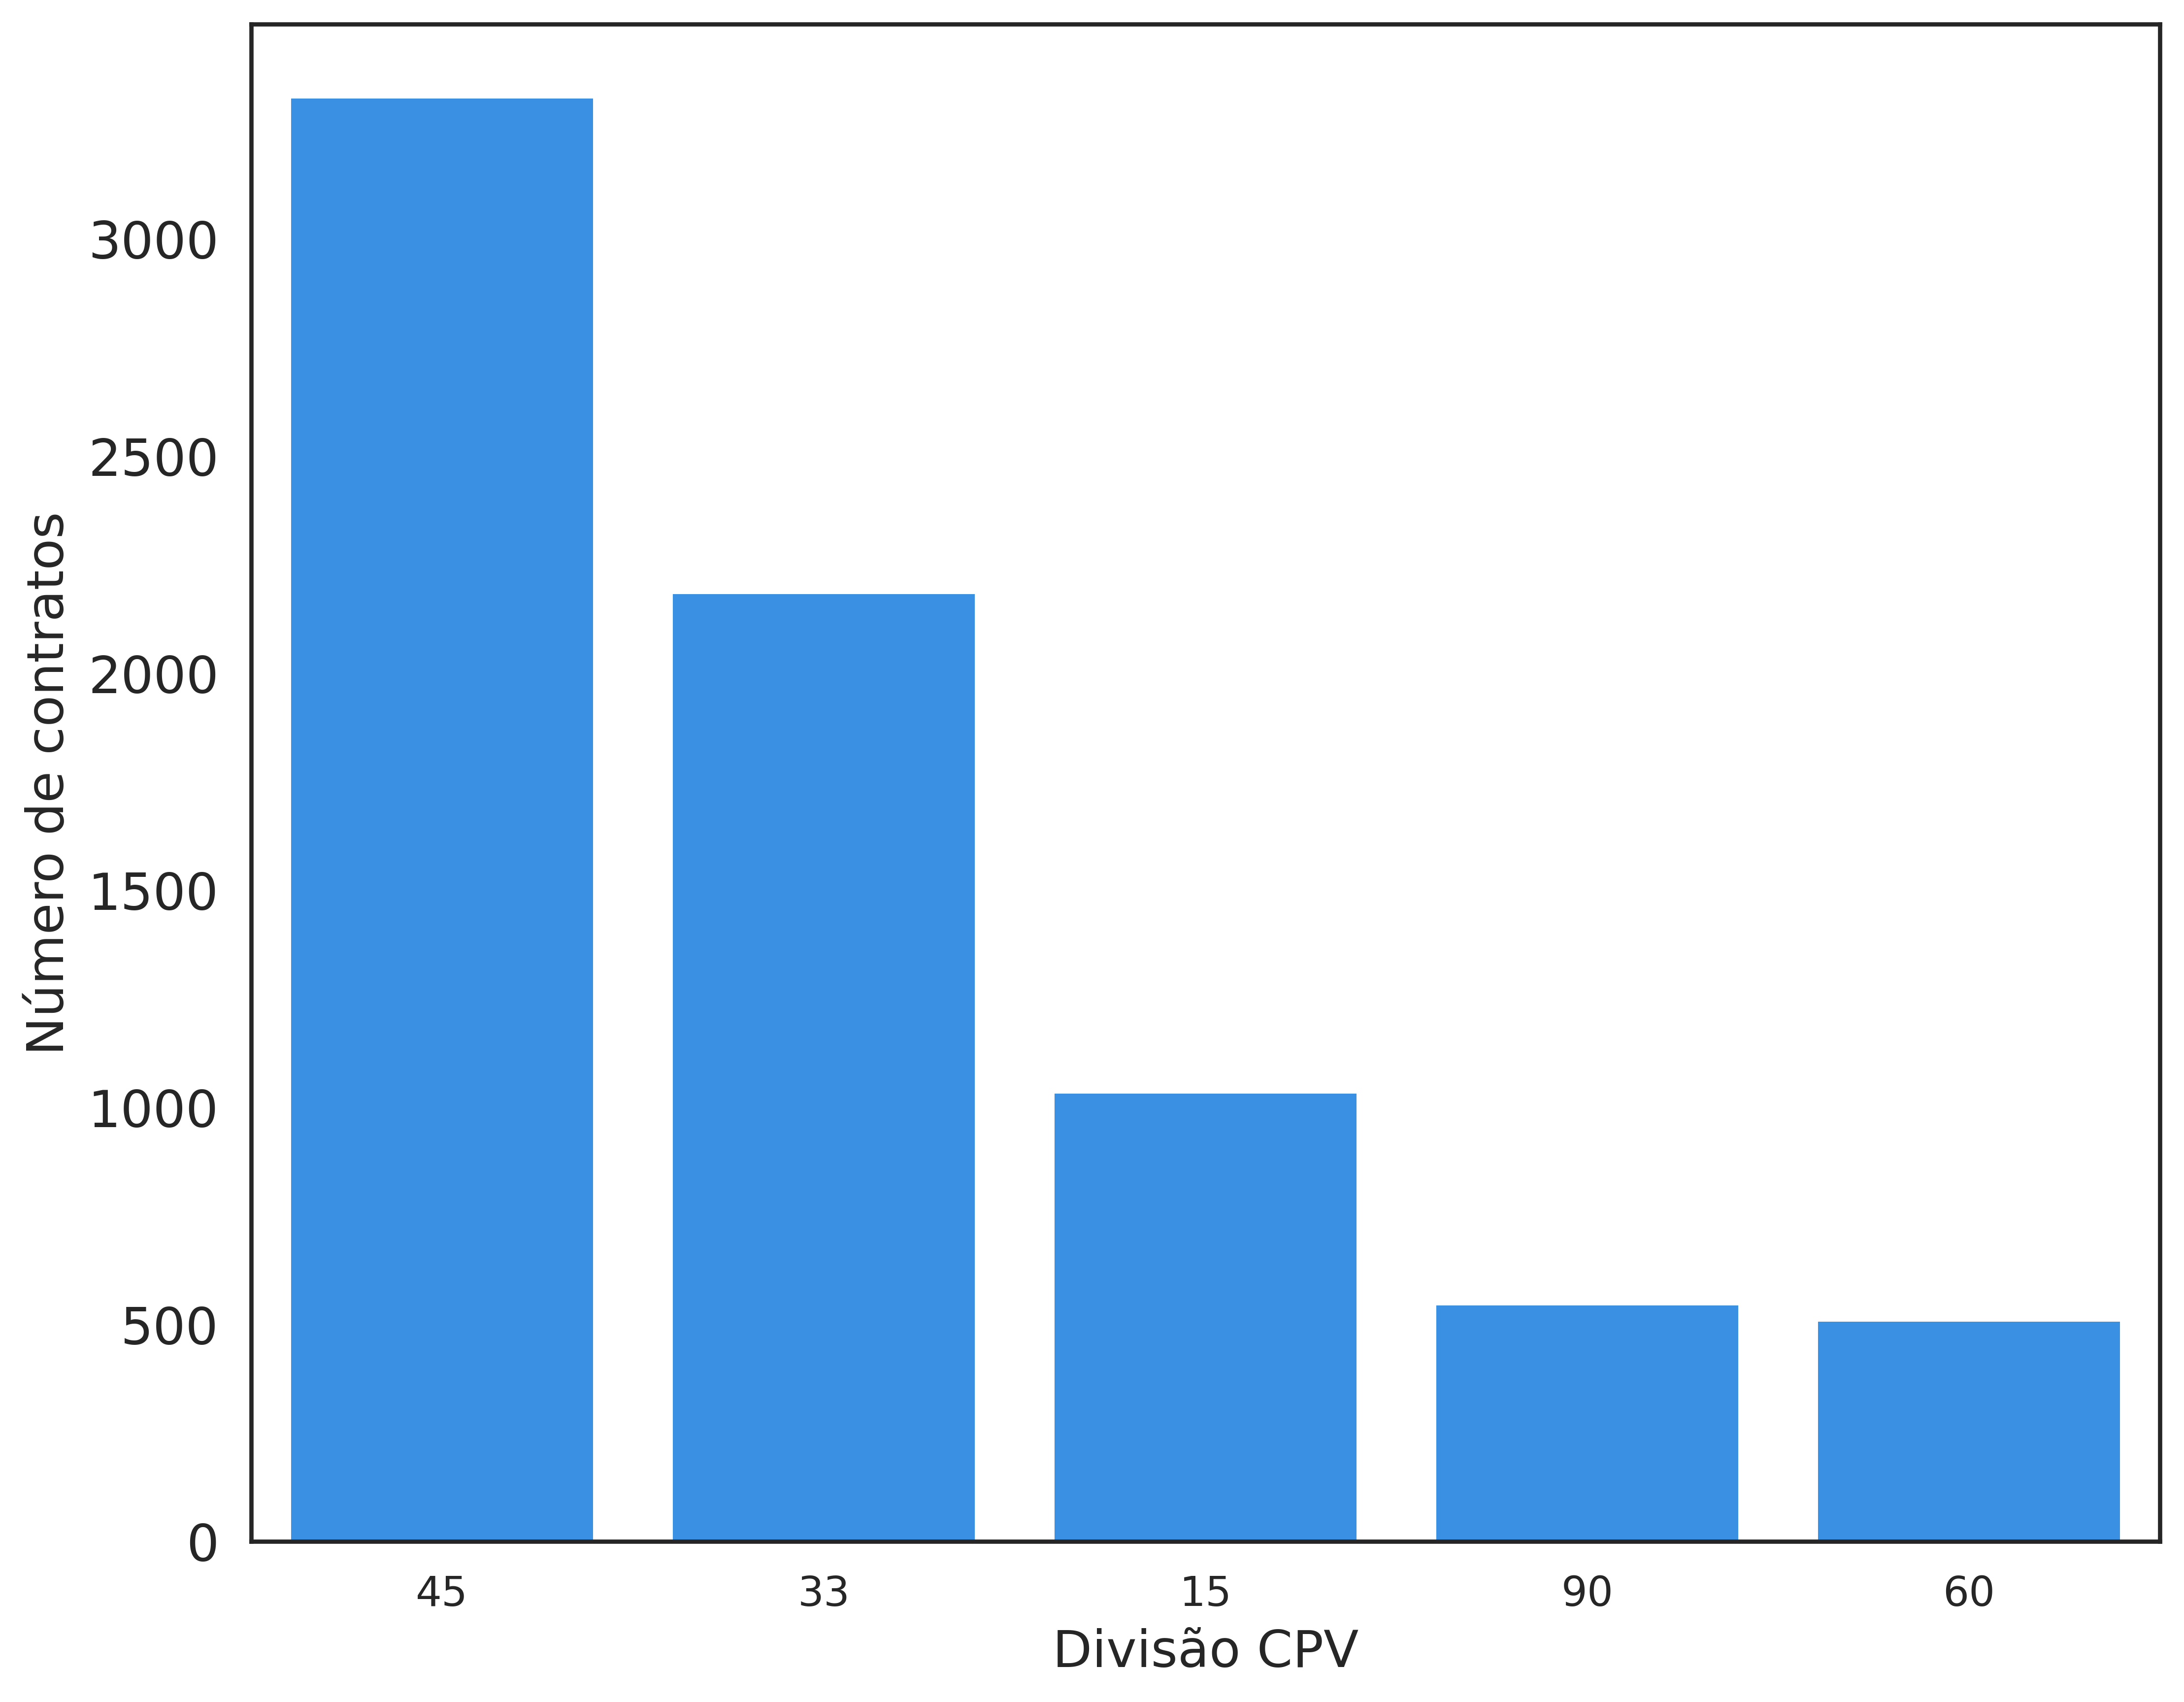
\includegraphics[width=0.5\textwidth]{imagens/rf2/main_cpvs.png}
%	\caption{Grupos com maior número de contratos indiciados}
%	\label{}
%\end{figure}

\begin{figure}[H]
	\centering
	\begin{minipage}{.45\linewidth}
		\begin{lstlisting}[
			language=SQL,
			showspaces=false,
			basicstyle=\ttfamily,
			numbers=left,
			numberstyle=\tiny,
			commentstyle=\color{gray},	frame=single,
			breaklines=true,
			autogobble = true,
			postbreak=\mbox{\textcolor{red}{$\hookrightarrow$}\space},
			]
			SELECT contratos_basegov."id"
			
			FROM contratos_basegov 
			
			WHERE contratos_basegov."totalEffectivePrice" > 0 AND 
			ABS(contratos_basegov."totalEffectivePrice" - preco_contratual) > 0 AND 
			preco_contratual > 0;
		\end{lstlisting}
	\end{minipage}
	\hfill
	\begin{minipage}{.4\linewidth}
		\centering
		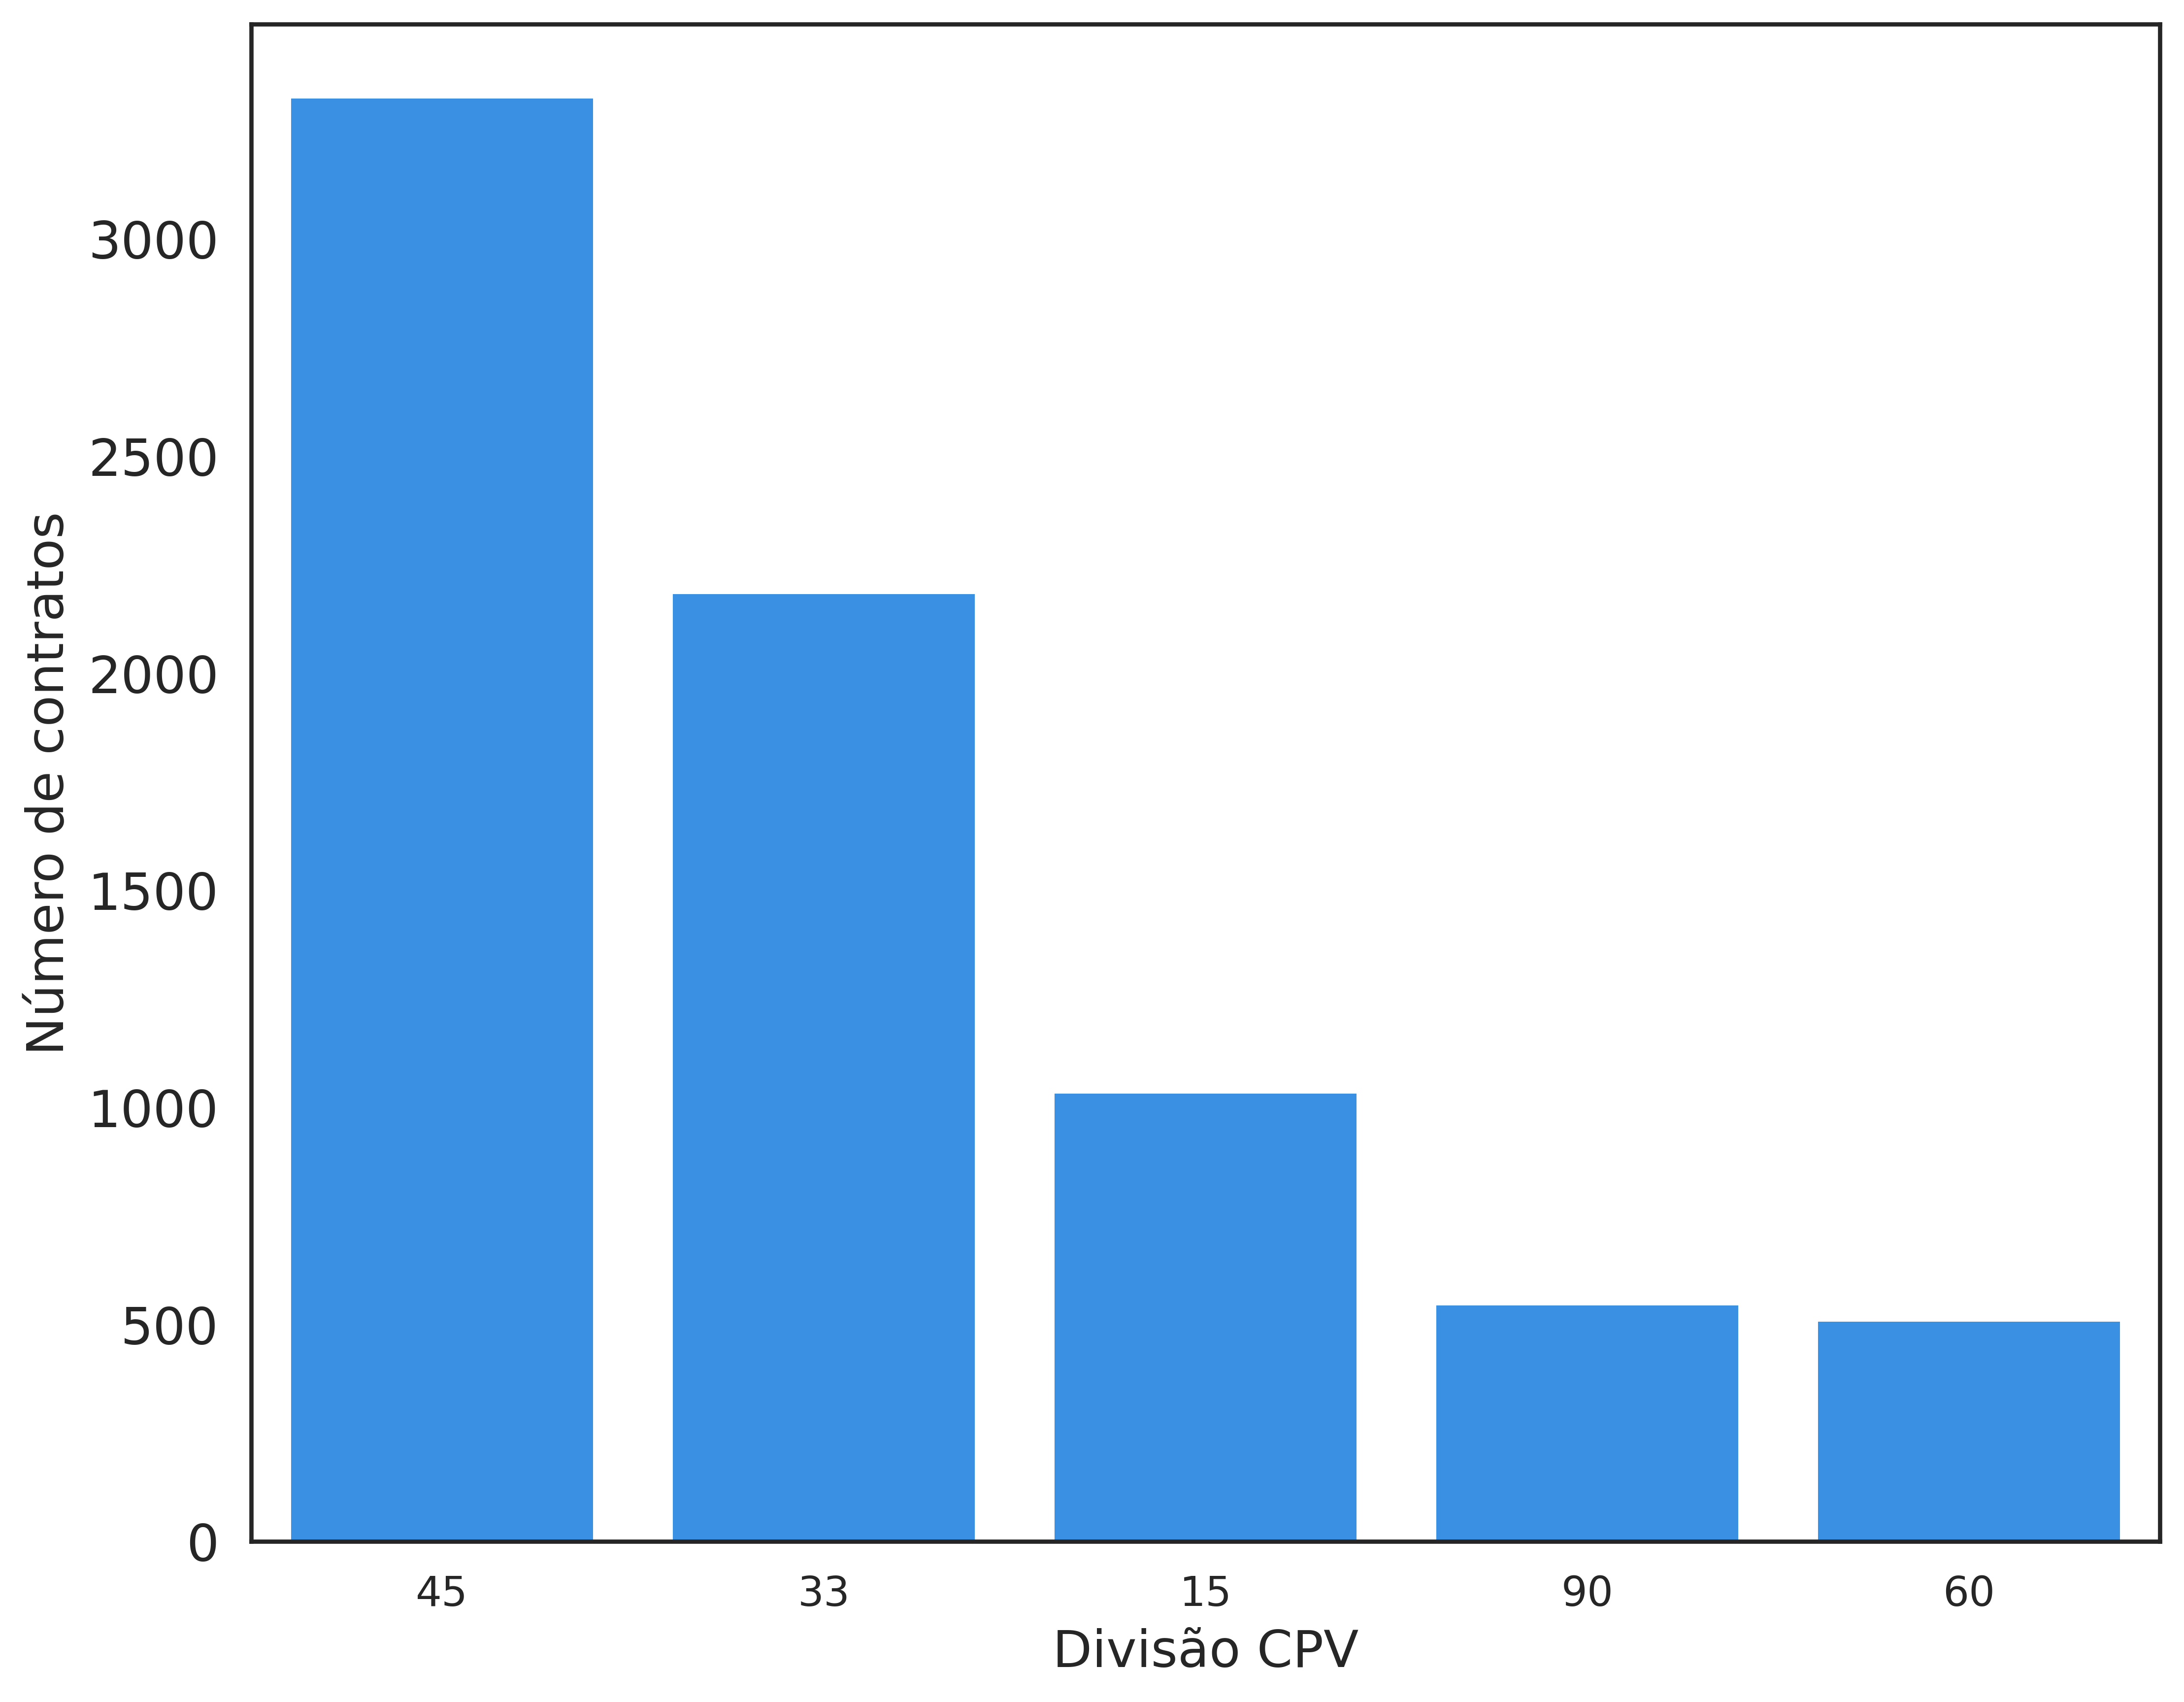
\includegraphics[width=\textwidth]{imagens/rf2/main_cpvs.png}
		\caption{Grupos do CPV com maior número de contratos sinalizados.}
		\label{}
	\end{minipage}
\end{figure}


\section{RF3: Análise da data de publicação do anúncio}

Adicionalmente, foi feita uma análise da data de publicação do anúncio em Diário da República. O objetivo deste indicador, cujo código se encontra disponível para consulta na Secção \ref{lst:rf3code}, é verificar a publicação de anúncios publicados em datas não convencionais - domingos e feriados nacionais - na tentativa de os fazer passar despercebidos. Não existe nenhuma ocorrência deste indicador nos contratos presentes na base de dados durante o período de tempo considerado. 



\section{Processo de automação}

Finda a construção dos indicadores, automatizou-se o processo de aplicação destes indicadores a todos os novos contratos que são adicionados diariamente à base de dados. Este processo foi aplicado somente a concursos públicos, tendo sido utilizadas todas as flags, exceto a R031 e R051. Primeiramente, construiu-se uma nova tabela, chamada \textit{daily\_flags}, com a configuração da Tabela \ref{tab:dailyexample}. 


\begin{table}[H]
	\centering
	\renewcommand{\arraystretch}{1.15}
	\setlength{\tabcolsep}{15pt}
	\resizebox{\textwidth}{!}{%
		\begin{tabular}{lllllllll}
			\toprule
			\textbf{ID}                  & \textbf{Data Publicação}       & \textbf{Verificação}     & \textbf{RF2}              & \textbf{RF3}              & \textbf{R003}             & \textbf{R017}            & \textbf{R018}             & \textbf{R019}            \\ \midrule
			\multicolumn{1}{c}{12345678} & \multicolumn{1}{c}{01/01/2024} & \multicolumn{1}{c}{true} & \multicolumn{1}{c}{false} & \multicolumn{1}{c}{false} & \multicolumn{1}{c}{false} & \multicolumn{1}{c}{true} & \multicolumn{1}{c}{false} & \multicolumn{1}{c}{true} \\ \bottomrule
		\end{tabular}%
	}
	\caption{Exemplo de aplicação de todos os indicadores binários a um concurso público.}
	\label{tab:dailyexample}
\end{table}

Esta tabela é constituída pelo identificador do contrato, a data de publicação, uma coluna de verificação - cujo propósito irá ser clarificado mais adiante - e as colunas referentes a cada uma das flags, cujo output é binário: \textit{true} ou \textit{false}. 


Ao longo do processo de automação, selecionam-se, diariamente, os novos concursos públicos adicionados à tabela principal \textit{contratos\_basegov}, copiam-se as colunas que contêm o identificador e a data de publicação dos mesmos, aplicam-se as flags e insere-se o respetivo output nesta nova tabela. 


Antes de executar o software necessário para realizar este procedimento com sucesso, foram aplicados, manualmente, os indicadores presentes na Tabela \ref{tab:dailyexample} a todos os concursos públicos presentes na base de dados. Só após concluir este passo é que se deu início à execução do software responsável pelo processo de automatização. Na Figura \ref{fig:esquema} é possível observar um esquema panorâmico deste processo e das distintas etapas que o compõem.  


\begin{figure}[H]
	\centering
	
\includegraphics[width=\textwidth]{imagens/daily_flags_v2.png}
	\caption{Esquema do processo de automatização.}
	\label{fig:esquema}
\end{figure}


Este procedimento obedece a duas fases distintas. 

A primeira inicia-se com o desenvolvimento de quatro ficheiros criados em python, cada um deles com um objetivo específico, descritos a seguir. 

No ficheiro \textbf{table\_update.py} são definidas as funções responsáveis por atualizar e realizar as operações intermédias necessárias na tabela auxiliar \textit{concursos\_publicos}. Começa-se por definir uma função que verifica qual foi o último \textit{id} a ser copiado para esta tabela, evitando-se, assim, a duplicação de contratos. De seguida, são construídas funções com o objetivo de :

\begin{my_enumerate}
	
	\item Copiar as colunas \textit{id}, \textit{data\_publicacao}, 	\textit{contractTypes}, \textit{fundamentacao}, \textit{entidade\_adjudicante}, \textit{entidades\_contratadas}, \textit{entidades\_concorrentes}, \textit{executionPlace}, \textit{cpv} e \textit{preco\_contratual} dos novos contratos da tabela original.
	
	\item Fazer a separação das colunas \textit{entidade\_adjudicante} e \textit{entidades\_contratadas}.
	
	\item Fazer o cálculo do número de entidades concorrentes.
	
	\item Fazer a classificação dos contratos de acordo com a tipologia: \textbf{Bens e Serviços} ou \textbf{Empreitadas}.
	
\end{my_enumerate}



No ficheiro \textbf{flag\_calculator.py} são definidas todas as funções responsáveis por calcular os indicadores presentes na Tabela \ref{tab:dailyexample}. Para tal, utilizou-se a biblioteca \textit{psycopg2} que permite realizar a conexão entre o python e base de dados. As funções definidas, não só são responsáveis por calcular o output de um determinado indicador para um contrato, como também, atualizar a tabela \textit{daily\_flags} com o resultado final. Por fim, foi criada uma função global que sistematiza o cálculo de todas as flags numa única função.

Em \textbf{process\_update.py} são invocadas todas as funções desenvolvidas nos ficheiros \textbf{flag\_calculator.py} e \textbf{table\_update.py}. Neste caso, começa por se aplicar as funções desenvolvidas no primeiro ficheiro e, só de seguida, as do último. Se o processo de cálculo das flags ocorrer com sucesso, é atribuído um valor \textit{true} na coluna de verificação para todos os contratos considerados. Esta coluna funciona como um mecanismo de prevenção para a eventualidade de o processo não decorrer como suposto. 

Quando ocorre alguma anomalia e este processo não decorre como planeado, a coluna de verificação assume o valor \textit{false}. Nessas situações são invocadas as funções do ficheiro \textbf{none\_cases.py}. Inicialmente, são identificadas todas as entradas da tabela \textit{daily\_flags} que contenham o valor \textit{false} nesta coluna. De seguida, procede-se à remoção das mesmas e, por fim, repete-se todo o processo descrito anteriormente.


%Começa-se por criar uma imagem em Docker com os ficheiros desenvolvidos. De seguida, no serviço de cloud AWS, foi criado um repositório, num Elastic Container Register (ECR), onde se armazenou a imagem Docker. Para executar os ficheiros presentes nesta imagem, foi criada uma função Lambda que guarda o output na tabela \textit{daily\_flags} da base de dados. Por fim, de forma a executar este processo de forma diária, foi programada uma calendarização do mesmo através do AWS Event Bridge. 



Após a construção destes ficheiros, dá-se início à segunda fase. Nesta, são utilizadas ferramentas que executam, de forma automática e sem qualquer tipo de intervenção manual, todos os ficheiros referidos anteriormente.

Para implementar este processo, começa por se criar uma imagem Docker com os ficheiros desenvolvidos. O Docker é uma plataforma que permite criar, executar e gerir aplicações em \textit{containers}, que, em suma, são unidades de \textit{software} que incluem todas as funcionalidades que uma aplicação necessita para funcionar corretamente: o código, runtime, ferramentas do sistema e bibliotecas.

A seguir, no serviço de cloud AWS, foi criado um repositório no Elastic Container Registry (ECR), onde a imagem Docker foi armazenada. Para executar os ficheiros presentes nesta imagem, foi criada uma função Lambda que guarda o output na tabela \textit{daily\_flags} da base de dados. Por fim, de forma a garantir que este processo é executado diariamente, foi programada uma calendarização do mesmo através do serviço AWS Event Bridge. 


































